\documentclass[a4paper,10pt]{book}
\linespread{1.5}
\setlength{\parindent}{0cm}
\usepackage[latin1]{inputenc}
\usepackage[spanish]{babel}
\usepackage{amssymb}
\usepackage{textcomp}
\usepackage{amsmath}
\usepackage{wrapfig}
\usepackage{pgf,tikz}
\usepackage{pstricks-add}
\usepackage{graphicx}
\usepackage{hyperref}
\usepackage{verbatim}
\usepackage{makeidx}
\usepackage{multirow} %Tablas
\usepackage{listings} %Escribir código.
\usepackage{color}    %Color en el código
\usepackage{todonotes}
\usepackage{url}

\definecolor{miverde}{rgb}{0,0.6,0}
\definecolor{migris}{rgb}{0.5,0.5,0.5}
\definecolor{mimalva}{rgb}{0.58,0,0.82}

\lstset{ %
  backgroundcolor=\color{white},   % Indica el color de fondo; necesita que se añada \usepackage{color} o \usepackage{xcolor}
  basicstyle=\footnotesize,        % Fija el tamaño del tipo de letra utilizado para el código
  breakatwhitespace=false,         % Activarlo para que los saltos automáticos solo se apliquen en los espacios en blanco
  breaklines=true,                 % Activa el salto de línea automático
  captionpos=b,                    % Establece la posición de la leyenda del cuadro de código
  commentstyle=\color{miverde},    % Estilo de los comentarios
  deletekeywords={...},            % Si se quiere eliminar palabras clave del lenguaje
  escapeinside={\%*}{*)},          % Si quieres incorporar LaTeX dentro del propio código
  extendedchars=true,              % Permite utilizar caracteres extendidos no-ASCII; solo funciona para codificaciones de 8-bits; para UTF-8 no funciona. En xelatex necesita estar a true para que funcione.
  frame=single,	                   % Añade un marco al código
  keepspaces=true,                 % Mantiene los espacios en el texto. Es útil para mantener la indentación del código(puede necesitar columns=flexible).
  keywordstyle=\color{blue},       % estilo de las palabras clave
  language=Python,                 % El lenguaje del código
  otherkeywords={*,...},           % Si se quieren añadir otras palabras clave al lenguaje
  numbers=left,                    % Posición de los números de línea (none, left, right).
  numbersep=5pt,                   % Distancia de los números de línea al código
  numberstyle=\small\color{migris}, % Estilo para los números de línea
  rulecolor=\color{black},         % Si no se activa, el color del marco puede cambiar en los saltos de línea entre textos que sea de otro color, por ejemplo, los comentarios, que están en verde en este ejemplo
  showspaces=false,                % Si se activa, muestra los espacios con guiones bajos; sustituye a 'showstringspaces'
  showstringspaces=false,          % subraya solamente los espacios que estén en una cadena de esto
  showtabs=true,                  % muestra las tabulaciones que existan en cadenas de texto con guión bajo
  stepnumber=0,                    % Muestra solamente los números de línea que corresponden a cada salto. En este caso: 1,3,5,...
  stringstyle=\color{mimalva},     % Estilo de las cadenas de texto
  tabsize=2,	                   % Establece el salto de las tabulaciones a 2 espacios
  title=\lstname                   % muestra el nombre de los ficheros incluidos al utilizar \lstinputlisting; también se puede utilizar en el parámetro caption
}


\makeindex
\newtheorem{teo}{Teorema}[chapter]
\newtheorem{propo}{Proposici\'on}[chapter]
\newtheorem{obs}{Observaci\'on}
\newtheorem{dem}{Demostraci\'on}
\newtheorem{definicion}{Definici\'on}[chapter]
\newtheorem{lema}{Lema}[chapter]
\newtheorem{coro}{Corolario}[chapter]
\newtheorem{eje}{Ejemplo}[chapter]


\begin{document}

\begin{titlepage}
\thispagestyle{empty}
\begin{center}
    
\includegraphics[height=2.6cm]{unam_oficial.png}
\end{center}
\begin{center}
    \textbf{\small UNIVERSIDAD NACIONAL AUT\'ONOMA DE M\'EXICO}\\
    {\footnotesize PROGRAMA DE MAESTR\'IA Y DOCTORADO EN CIENCIAS MATEM\'ATICAS Y DE LA ESPECIALIZACI\'ON EN ESTAD\'ISTICA APLICADA}
\end{center}
\vspace{1cm}
\begin{center}
    \textit{\small Estructuras de Poisson en Foliaciones de Bott-Morse en Dimensi\'on Tres}
\end{center}
\vspace{1cm}
\begin{center}
    {\footnotesize TESIS\\ 
    QUE PARA OPTAR POR EL GRADO DE: \\
    MAESTRO EN CIENCIAS} 
\end{center}
\vspace{1cm}
\begin{center}
    {\footnotesize PRESENTA:\\
    MIGUEL ANGEL EVANGELISTA ALVARADO}
\end{center}
\vspace{1cm}
\begin{center}
    {\footnotesize DIRECTOR:\\
    DR. PABLO SU\'AREZ SERRATO\\
    INSTITUTO DE MATEM\'ATICAS-CU\\
    UNAM}
\end{center}
\vspace{1cm}
\begin{center}
    {\footnotesize CIUDAD DE M\'EXICO A 6 DE SEPTIEMBRE DE 2019.}     
\end{center}

%% Barra izquierda - Escudos
%%\hskip -2cm
%%\begin{minipage}[c][10cm][s]{3cm}
%%  \begin{center}
%%    
\includegraphics[height=2.6cm]{logoUNAM.png}\\[10pt]
%%    \hskip2pt\vrule width2.5pt height13cm\hskip1mm
%%    \vrule width1pt height13cm\\[10pt]
%%    
\includegraphics[height=2.6cm]{logoIMATE.png}
%%  \end{center}
%%\end{minipage}\quad
%% Barra derecha - Títulos
%%\begin{minipage}[c][9.5cm][s]{11cm}
%%  \begin{center}
%%    % Barra superior
%%    {\large \scshape Universidad Nacional Aut\'onoma de M\'exico}
%%    \vspace{.3cm}
%%    \hrule height4pt
%%    \vspace{.1cm}
%%    \hrule height3pt
%%    \vspace{.3cm}
%%    {\scshape  Instituto de Matem\'aticas}\\
%%    \vspace{.3cm}
%%    % Título del trabajo
%%    \vspace{2cm}
%%    {\Large \scshape {Estructuras de Poisson en Foliaciones de Bott-Morse en dimensi\'on tres}}\\
%%    \vspace{2cm}
%%    % Tipo de trabajo
%%    \makebox[5cm][s]{\Huge T E S I S}\\[6pt]
%%    PARA OBTENER EL T\'ITULO DE:\\[5pt]
%%    \textbf{Maestro en Ciencias Matem\'aticas}\\[40pt]
%%    PRESENTA:\\[5pt]
%%    \textbf{Miguel Angel Evangelista Alvarado}\\
%%    \vspace{1cm}
%%    {\small DIRECTOR DE TESIS:\\ Dr. Pablo Su\'arez Serrato}\\
    %\vspace{0.5cm}
    %{\small CO-DIRECTOR DE TESIS:\\ Dr. Walter Carballosa Torres}\\
%%    \vspace{1.5cm}
%%    \rightline{Cuidad de M\'exico, M\'exico 2019.}
    
%%  \end{center}
%%\end{minipage}
\end{titlepage}

\chapter*{}
\pagenumbering{roman} % para comenzar la numeracion de paginas en numeros romanos
\begin{flushright}
\textit{Dedicado a \\
Mi compa\~{n}era de vida {\bfseries Gabriela}.}
\end{flushright}

\chapter*{Agradecimientos} % si no queremos que añada la palabra "Capitulo"
\addcontentsline{toc}{chapter}{Agradecimientos} % si queremos que aparezca en el índice
\markboth{AGRADECIMIENTOS}{AGRADECIMIENTOS} % encabezado 

A mi padre Joaqu\'in Evangelista, del cual siempre he recibido sabios consejos para afrontar la vida, a mi madre Marina Alvarado qui\'en siempre me motivo a seguir adelante con mis estudios de maestr\'ia y a no renunciar a mis sue\~{n}os, ella es mi ejemplo a seguir, y es la persona que m\'as admiro. Los amo.\\ 

\par A mi amada esposa Gabriela Bail\'on Solano, por ser parte muy importante de mi vida, por brindarme su apoyo en las buenas y en las malas durante esta traves\'ia, pero sobre agradezco su infinito amor y compresi\'on. Te Amo.\\

\par Al Dr. Pablo Su\'arez Serrato, director del trabajo realizado, por la confianza depositada en mi desde mis estuidos de licenciatura, as\'i como la orientaci\'on, el seguimiento y la supervici\'on contin\'ua durante la realizacion de la maestr\'ia y de este trabajo.\\   

\par A mis sinodales el Dr. H\'ector S\'anchez quien adem\'as fue mi profesor de Geometr\'ia Diferencial, el Dr. Misael Avenda\~{n}o, el Dr. Jose Ru\'iz y la Dra. Laura Ort\'iz por la minusiosa revisi\'on y el tiempo dedicado a este trabajo. As\'i como a sus atinadas observaciones.\\    

\par A mi hermano Juan Mart\'in y su esposa Rub\'i por ser parte importante en mi familia y en especial a mis sobrinos Alexis Paul y Cristian Neri que iluminan mis dias cuando los veo.\\     

\par A cada uno de los integrates de la famila Bail\'on Solano por haberme aceptado como un miembro m\'as de su familia y mostrarme siempre su apoyo incondicional.\\

\par A todos y cada uno de mis compa\~{n}eros: Luis, Pedro, Oscar, Jimmy, Gil, Neto y Mario con los cuales pasamos momentos agradables y nos motivavamos cuando la situacion estaba un poco dificil o nos ibamos a echar la cascara. As\'i como a mis hermanos acad\'emicos Eduardo y Haydee los cuales me acompa\~{n}aron durante mi traves\'ia en el Instituto de Matem\'aticas.\\

\par Al apoyo econ\'omico que me brindo la beca CONACYT y la beca del PAPIIT de la Universidad Nacional Aut\'onoma de M\'exico para la realizaci\'on del presente trabajo. \newline
\rightline{Miguel Angel Evangelista Alvarado.}\newline
\leftline{Cuidad Universitaria, CDMX a \today.}                

\tableofcontents
%\listoffigures %índice de figuras

\chapter*{Introducci\'on}
\addcontentsline{toc}{chapter}{Introducci\'on}
   
El presente trabajo tiene como finalidad construir estructuras de Poisson adaptadas a foliaciones de Bott-Morse de codimensi\'on uno en variedades lisas de dimensi\'on tres. Para lo anterior retomamos ideas y resultados obtenidos por Su\'arez y Orozco en \cite{SO}, Su\'arez, Garc\'ia y Vera en \cite{GSV}, y Sc\'ardua y Seade en \cite{Seade1}.
\vspace{5mm}

El resultado principal de esta tesis es demostrar el siguiente teorema, que se encuentra en la Secci\'on \ref{3.2} del Cap\'itulo \ref{cap3}.\\

\textbf{Teorema.} \textit{Sea $\mathcal{F}$ una foliaci\'on lisa y compacta de codimensi\'on uno con singularidades de Bott-Morse sobre una variedad lisa, conexa, cerrada y orientable $M^{3}$, y $f:M\to\mathbb{R}$ el mapeo de Bott-Morse que da lugar a $\mathcal{F}$. Entonces, existe una estructura de Poisson completa en $M^{3}$ de rango dos tal que el tensor de Poisson asociado a \'esta estructura solo se anula en dos puntos o en dos c\'irculos que corresponden exactamente a la singularidades de las foliaci\'on $\mathcal{F}$.}\\
 
Este trabajo se estructura en tres cap\'itulos y un ap\'endice. El Cap\'itulo \ref{cap1} explica uno de los pilares de este trabajo de investigaci\'on que son las foliaciones de Bott-Morse de codimensi\'on uno, para entender lo anterior describimos las nociones b\'asicas de la teor\'ia de foliaciones singulares en la Secci\'on \ref{1.1} y a la teor\'ia de Morse en la Secci\'on \ref{1.2}, para as\'i llegar al concepto de foliaciones de Bott-Morse de codimensi\'on uno en la Secci\'on \ref{1.3}, esto basado en los art\'iculos de Sc\'ardua y Seade en \cite{Seade1} y \cite{Seade2}.  
\vspace{5mm}

El Cap\'itulo \ref{cap2} muestra puntualmente el segundo y \'ultimo pilar de este trabajo de investigaci\'on, que es la geometr\'ia de Poisson; retomando los conceptos de campos multivectoriales en la Secci\'on \ref{2.1}, de variedades de Poisson en la Secci\'on \ref{2.2} y finalmente en la Secci\'on \ref{2.3} demostramos que toda variedad de Poisson tiene asociada una foliaci\'on donde las hojas son variedades simpl\'ecticas y se enuncia el teorema \ref{TeoGSV} el cual contiene la f\'ormula de Flashka-Ratiu, que sirve para construir estructuras de Poisson.
\vspace{5mm}         

El Cap\'itulo \ref{cap3} tiene como objetivo hacer converger las ideas expresadas en los Cap\'itulos \ref{cap1} y \ref{cap2}, para as\'i construir las estructuras de Poisson de manera local en una singularidad de la foliaci\'on de Bott-Morse. Despu\'es extenderemos la estructura de Poisson encontrada en la Secci\'on \ref{3.1} a toda la variedad. Esto lo realizamos en la Secci\'on \ref{3.2} y por \'ultimo, en la Secci\'on \ref{3.3}, explicamos como son las formas simpl\'ecticas inducidas por las estructuras de Poisson encontradas en la Secci\'on \ref{3.1}.
\vspace{5mm}

En el Ap\'endice \ref{A1} explicamos scripts escritos en lenguaje Python, los cuales utilizamos para realizar c\'alculo simb\'olico. Estos c\'alculos son: la f\'ormula de Flaska-Ratiu para encontrar estructuras de Poisson en la Secci\'on \ref{A.1}, un m\'etodo para encontrar estructuras simpl\'ecticas inducidas por la estructuras de Poisson en la Secci\'on \ref{A.2} y por \'ultimo la f\'ormula para calcular el corchete de Schouten-Nijenhuis en la Secci\'on \ref{A.3}, de este modo incursionamos en la Geometr\'ia de Poisson computacional. % Listo

\chapter{Foliaciones de Bott-Morse}\label{cap1}%
\pagenumbering{arabic}

Esta investigaci\'on inicia con la presentaci\'on de un panorama b\'asico a la teor\'ia de foliaciones con singularidades de Bott-Morse. La idea es explicar las nociones b\'asicas de \'esta teor\'ia, la cual usaremos en los resultados presentados en el Cap\'itulo \ref{cap3}.\\

A lo largo de este trabajo de investigaci\'on se considera que las variaedades diferenciables $M$ son de dimensi\'on $m$ y son de clase $C^{\infty}$, solo en caso de ser requerida una adecuaci\'on se especificar\'a. Adem\'as se considera un {\bfseries mapeo liso} de clase $C^{k}$ \'o simplemente liso a un mapeo $f:M\to N$ tal que para todo $p\in M$ se cumple que $\psi\circ f\circ\phi^{-1}$ es de clase $C^{k}$ en $0$, donde $(V_{p},\psi)$ es una carta de $M$ y $(V_{f(p)},\phi)$ es una carta de $N$ con $f(p)=0$. Si $f$ es liso escribimos $f\in C^{k}(M,N)$ y cuando $N=\mathbb{R}$, denotamos $C^{k}(M,N)$ por $C^{k}(M)$.       

\section{Foliaciones}\label{1.1}
Iniciamos la secci\'on con un breve repaso a la teor\'ia de foliaciones. Para realizar un estudio detallado de esta teor\'ia recomendamos al lector dirigirse a los siguientes textos \cite{Camacho} o \cite{Molino}. \\

Para explicar de manera intuitiva el concepto de foliaci\'on, hay que recordar que al integrar un campo vectorial no singular sobre una variedad $M$, obtenemos una partici\'on de la variedad $M$ mediante integrales del campo, que son variedades diferenciables de dimensi\'on uno. A esta partici\'on la llamaremos foliaci\'on de $M$ de dimension uno y a las \'orbitas del flujo del campo como hojas de la foliaci\'on. \\

La forma natural de generalizar lo anterior a dimensiones superiores, es considerar la soluci\'on de un sistema de ecuaciones diferenciales sobre una variedad bajo una condici\'on de integrabilidad, es decir, el teorema de Frobenius.\\

A continuaci\'on enunciamos la definici\'on de foliaci\'on.

\begin{definicion}\label{def1}
Sea $M^{m}$ una variedad, decimos que una {\bf foliaci\'on} en $M^{m}$ de dimensi\'on $n$ es un atlas $\mathcal{F}$ en $M$ que cumple con las siguientes propiedades:
\begin{enumerate}
	\item Si $(U,\varphi)\in\mathcal{F}$, entonces $\varphi:U\to \bar{U}_{1}\times \bar{U}_{2}\subset\mathbb{R}^{n}\times\mathbb{R}^{m-n}$, donde $\bar{U}_{1}\subset\mathbb{R}^{n}$ y $\bar{U}_{2}\subset\mathbb{R}^{m-n}$ son discos abiertos.
	\item Si $(U_{1},\varphi_{1})$ y $(U_{2},\varphi_{2})\in\mathcal{F}$ tal que $U_{1}\cap U_{2}\neq \emptyset$, entonces la funci\'on de transici\'on $\varphi_{2}\circ\varphi_{1}^{-1}: \varphi_{1}(U_{1}\cap U_{2})\to\varphi_{2}(U_{1}\cap U_{2})$, es de la forma 	$(f_{1}(x,y),f_{2}(y))$ para $(x,y)\in\varphi_{1}(U_{1}\cap U_{2})$ y algunas funciones lisas $f_{1}:\mathbb{R}^{m}\to\mathbb{R}^{m}$ y $f_{2}:\mathbb{R}^{m-n}\to\mathbb{R}^{m-n}$. 	
\end{enumerate} 
\begin{figure}[!ht]
\centering
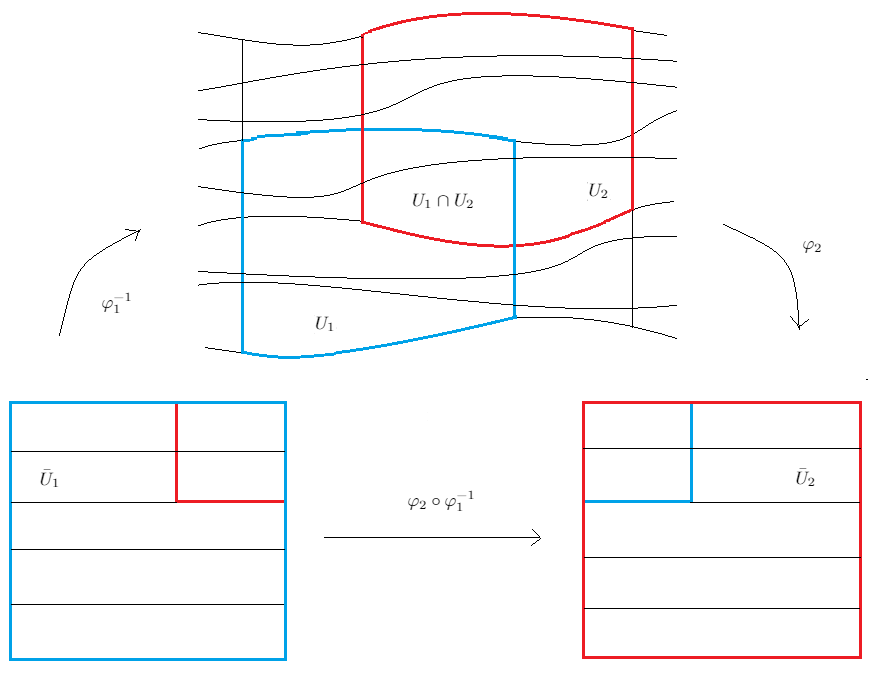
\includegraphics[scale=0.5]{foliacion.png}
\caption{Una $2-$variedad foliada por una $1-$variedad.}
\label{foliacion}
\end{figure}
\end{definicion}

Para poder tener clara la definici\'on \ref{def1} siempre podemos pensar en la figura \ref{foliacion}, que es una variedad de dimensi\'on dos foliada por una variedad de dimensi\'on uno.\\

A las cartas $(U,\varphi)\in\mathcal{F}$ las llamamos {\bfseries cartas foliadas} y el n\'umero $m-n$ se conoce como codimensi\'on de la folicai\'on.\\

Considere una foliaci\'on $\mathcal{F}$ en $M^{m}$ de dimension $n$ tal que $n<m$. Si seleccionamos un carta foliada $(U,\varphi)\in\mathcal{F}$ y fijamos un $c\in\bar{U}_{2}$, podemos considerar lo siguiente:
\begin{itemize}
	\item el conjunto $\varphi^{-1}(\bar{U}_{1}\times\{c\})$ es llamado {\bfseries placas} de $U$ o de $\mathcal{F}$ esto depende del contexto, y        
	\item el mapeo $\varphi|_{\bar{U}_{1}\times\{c\}}:\bar{U}_{1}\times\{c\}\to U$ resulta ser un encaje, as\'i las placas son subvariedades conexas de $M^{m}$ con dimensi\'on $n$.
\end{itemize}

Observar que para $c\in\bar{U}_{2}$ se obtienen placas de $U$ ajenas, para esto considere $c_{1}$ y $c_{2}\in\bar{U}_{2}$ tal que $c_{1}\neq c_{2}$ y sus respectivas placas $\alpha=\varphi^{-1}(\bar{U}_{1}\times\{c_{1}\})$ y $\beta=\varphi^{-1}(\bar{U}_{1}\times\{c_{2}\})$. Ahora supongamos que $\alpha\cap\beta\neq\emptyset$, entonces:
\[ \begin{array}{ccccc}
	(\alpha\cap\beta) & = & \bar{U}_{1}\times\{c_{1}\} & pues & \alpha\cap\beta\subset\alpha \\  
					  & = & \bar{U}_{1}\times\{c_{2}\} & pues & \alpha\cap\beta\subset\beta,  
   \end{array} \]
pero $(\bar{U}_{1}\times\{c_{1}\})\neq(\bar{U}_{1}\times\{c_{2}\})$, por lo tanto $\alpha\cap\beta=\emptyset$. \\

Un {\bfseries camino de placas} de $\mathcal{F}$ es un sucesi\'on $\{\alpha_{1},...,\alpha_{k}\}$ de placas de $\mathcal{F}$ tal que $\alpha_{i}\cap\alpha_{i+1}\neq 0$ para $i\in\{1,...,k-1\}$.\\ 

Dado que es posible cubrir a $M^{m}$ por placas de $\mathcal{F}$, definimos la siguiente relaci\'on de equivalencia: Para $p,q\in M^{m}$ decimos que $p\sim q$ si y s\'olo si existe un camino de placas $\{\alpha_{1},...,\alpha_{k}\}$ tal que $p\in\alpha_{1}$ y $q\in\alpha_{k}$. A la clases de equivalencia la llamamos {\bfseries hojas} de $\mathcal{F}$ y al conjunto $M/\sim$ el {\bfseries espacio de hojas}. \\

Se tiene por definici\'on que las hojas de $\mathcal{F}$ son un subconjunto conexo por trayectorias y que por cada punto $p\in M^{m}$ pasa una y s\'olo una hoja de $\mathcal{F}$. Adem\'as una propiedad de las hojas de $\mathcal{F}$ no tan inmediata de su definici\'on, es que estas son variedades diferenciables de dimensi\'on $n$ y de clase $r$, cuya estructura diferenciable la heredan de $\mathcal{F}$. La prueba de lo anterior se puede consultar en [P\'agina 32, \cite{Camacho}].\\

Decimos que una {\bfseries foliaci\'on $\mathcal{F}$ es compacta} si cada hoja $L\in\mathcal{F}$ es compacta y de manera similar decimos que una {\bfseries foliaci\'on $\mathcal{F}$ es cerrada} si cada hoja $L\in\mathcal{F}$ es cerrada.\\

Con todo lo anterior, se tiene que una foliaci\'on es un descomposici\'on de una variedad lisa en subvariedades de la misma dimensi\'on, es decir una foliaci\'on regular. Ahora, ?` Qu\'e ocurre cuando tenemos una descomposici\'on de $M$ en subvariedades pero la dimensi\'on estas var\'ian? Para explicar lo anterior debemos extender el concepto de foliaci\'on regular a singular.\\

Una {\bfseries foliaci\'on lisa $\mathcal{F}$ singular} en una variedad lisa $M^{m}$ es una partici\'on 
\begin{equation*}
    \mathcal{F}=\bigcup\limits_{p\in M} L_{p}
\end{equation*}
donde se cumple que $L_{p}\cap L_{q}=\emptyset$ si $p\neq q$ y cada $L_{p}$ es una subvariedad lisa, encajada y conexa de $M^{m}$. A cada $L_{p}$ lo llamamos {\bfseries hoja} de $M^{m}$.\\

Adem\'as se cumple la siguiente propiedad: Para cada $p\in M$ existe una carta $(U_{p}, (y_{1},...,y_{m}))$ tal que para la hoja $L_{p}$ la componente conexa de $L_{p}\cap U_{p}$ esta  descrita por las ecuaciones $y_{d+1}=c_{d+1},...,=y_{m}=c_{m}$ donde $c_{d+1},...,c_{m}$ son constantes. La propiedad anterior es conocida como {\bfseries la propiedad de la foliaci\'on local}.\\

Si todas las hojas $L_{p}$ de un foliaci\'on singular $\mathcal{F}$ tienen la misma dimensi\'on entonces decimos que $\mathcal{F}$ es una {\bfseries foliaci\'on regular}.\\

Una {\bfseries distribuci\'on singular} en una variedad lisa $M^{m}$ es una asignaci\'on talque a cada punto $p\in M^{m}$ le asocia un subespacio vectorial $D_{p}\subset T_{p}M$. Notemos que la dimensi\'on de $D_{p}$ puede depender del punto $p$. \\

Una distribuci\'on singular $D$ en una variedad lisa $M^{m}$ es llamada lisa si para cada punto $p\in M$ y cualquier vector $X_{0}\in D$ existe un campo vectorial $X$ liso definido en una vecindad  $U_{p}$ de $p$ tal que $X(y)\in D_{y}$ para toda $y\in U_{p}$ y $X(p)=X_{0}$.\\

Si la dimensi\'on de la distribuci\'on en $p$ no depende del punto $p$, entonces se tiene que la distribuci\'on es un distribuci\'on regular lisa.\\

Ahora, de la propiedad de la foliaci\'on local se puede deducir que la distribuci\'on tangente $D^{\mathcal{F}}$ de una foliaci\'on singular es un distribuci\'on singular lisa [P\'agina 17,\cite{Dufour}], donde la distribuci\'on tangente $D^{\mathcal{F}}$ es la que asocia a cada punto $p\in M$ su espacio tangente $D_{p}^{\mathcal{F}}$ a la hoja $L_{p}$ en el punto $p$.Es decir, cada folicai\'on singular define una distribuci\'on singular. Es decir, cada folicai\'on singular define una distribuci\'on singular.\\

Sea $D$ una distriubuci\'on singular y lisa en la variedad lisa $M$. Una {\bfseries subvariedad integrable} $W$ de $D$ es una subvariedad encajada de $M$ tal que para cada $w\in W$ el espacio tangente $T_{w}W\subset D_{w}$ es un subespacio vectorial.\\

Una subvariedad integrable $W$ es llamada {\bfseries maximal}, si no est\'a contenida en ninguna otra subvariedad integrable; decimos que una subvariedad integrable es de {\bfseries dimensi\'on m\'axima} si su espacio tangente en cada punto $w\in W$ es exactamente $D_{w}$.\\

Decimos que una distribuci\'on lisa y singular $D$ en una variedad lisa $M$ es una {\bfseries distribuci\'on integrable}, si cada punto $p\in M$ est\'a contenido en un variedad integrable maximal de dimensi\'on m\'axima en $D$. \\

Sea $C$ una familia de campos vectoriales lisos definidos en $M$. Definimos una distribuci\'on singular suave $\hat{D}$ tal que a cada punto $p\in M$ le asigna el espacio $\hat{D}_{p}$, donde $\hat{D}_{p}$ es el espacio vectorial generado por los valores del punto $p$ es los campos vectoriales de $C$.  
\vspace{5mm}

% \todo{checar}
Sea $D$ una una distribuci\'on, decimos que $D$ es {\bfseries invariante} con respecto a la familia de campos vectoriales $C$, si es invariante con respecto a cada elemento de $C$.
\vspace{5mm}

Dados todos los conceptos anteriores, surge de manera natural la siguiente pregunta: ?` Cu\'ales son las condiciones para que una distribuci\'on singular lisa sea la distribuci\'on tangente de una foliaci\'on singular?
\vspace{5mm}

La respuesta a la pregunta anterior se encuentran en los resultados del trabajo de Stefan \cite{Stefan74} y Sussmann \cite{Sussmann73}, expresados en el siguiente teorema, cuya demostraci\'on podemos encontrar en [P\'agina 17, \cite{Dufour}].
\begin{teo}\label{teoSteSus}
Sea $D$ un distribuci\'on lisa y singular en un variedad lisa $M^{m}$. Entonces son equivalentes las siguientes condiciones:
\begin{description}
    \item[i)] $D$ es integrable.
    \item[ii)] $D$ es generado por un familia de campos vectoriales lisos y es invariante con respecto a dicha familia.
    \item[iii)] $D$ es la distribuci\'on tangente $D^{\mathcal{F}}$ de una foliaci\'on singular y lisa $\mathcal{F}$. 
\end{description}
\end{teo}

Una {\bfseries distribuci\'on involutiva} es una distribuci\'on $D$ tal que si $X$ e $Y$ son dos campos vectoriales lisos que son tangentes a $D$, entonces el corchete de Lie $[X,Y]$ es tangente a $D$ tambi\'en. Es claro del teorema \ref{teoSteSus} que si una distribuci\'on singular es integrable, entonces es involutiva.
\vspace{5mm}

Hay que notar que el teorema \ref{teoSteSus} es un generalizaci\'on del teorema de Frobenius para una distribuci\'on regular $D$.

\begin{teo}\label{TeoFro}
Si una distribuci\'on regular lisa es involutiva, entonces es integrable, es decir, la distribuci\'on es la tangente distribuci\'on de una foliaci\'on regular.  
\end{teo}

El teorema de Frobenuis es resultado cl\'asico en la literatura sobre foliaciones regulares. La prueba se puede consultar en [P\'agina 182, \cite{Camacho}] y mientras que la de integrabilidad de foliaciones singulares se puede encontrar la p\'agina 18 de \cite{Dufour}, es decir, podemos concluir que el teorema de Frobenius es un caso particular del teorema de Stefan-Sussmann \ref{teoSteSus}.

\section{Mapeos de Morse}\label{1.2}
La teor\'ia de Morse a grandes rasgos estudia la topolog\'ia de las variedades diferenciables a partir de los mapeos de Morse que se pueden definir sobre ellas, para un estudio a detalle sugerimos consultar \cite{Milnor} y \cite{Matsumoto}. 
\vspace{5mm}

La teor\'ia de Morse ha tenido una gran cantidad de aplicaciones, entre las cuales se pueden destacar la clasificaci\'on de las superficies compactas \cite{Xu} y el teorema del h-cobordismo \cite{MilnorH-C}, s\'olo por mencionar algunas.
\vspace{5mm} 

Comenzamos tomando una variedad diferenciable  $M^{m}$ y $f:M^{m}\to\mathbb{R}$ un mapeo liso, decimos que un punto $p\in M^{m}$ es un {\bfseries punto cr\'itico} de $f$ si la diferencial de $f$ en $p$ es nula. En caso contrario decimos que $p$ es un {\bfseries punto regular}.
\vspace{5mm}

Notemos que si tomamos una carta $(U,x)$ alrededor de $p$ y $p$ es un punto cr\'itico de $f$, entonces se tiene    
$$\frac{\partial f}{\partial x_{1}}(p)=...=\frac{\partial f}{\partial x_{n}}(p)=0.$$   
El n\'umero real $f(p)$ donde $p$ es un punto cr\'itico lo llamamos {\bfseries valor cr\'itico}.
\vspace{5mm}

La restricci\'on que le impondremos a un mapeo liso para que \'este sea de Morse har\'a que los mapeos tengan un comportamiento muy simple en sus puntos cr\'iticos, para esto introduciremos la noci\'on de \emph{segunda derivada} del mapeo $f$ en el punto $p\in M^{m}$.
\vspace{5mm}

Sean $p\in M$ y $v_{p},w_{p}\in T_{p}M$. Elijamos $X$ e $Y$ campo vectoriales en $M^{m}$ tales que $X(p)=v_{p}$ e $Y(p)=w_{p}$. Si $p$ es un punto cr\'itico de $f$ entonces es claro que $v_{p}(Y(f)))=w_{p}(X(f))$, ya que
\[ \begin{array}{ccl}
	v_{p}(Y(f))-w_{p}(X(f)) & = & X(p)(Y(f)))-Y(p)(X(f))\\
							 & = & [X,Y](p)(f) \\
							 & = & 0 
\end{array} \]
As\'i, podemos definir una forma bilineal $Hess_{p}(f)$ en $T_{p}M$ llamada el hessiano de $f$ en el punto $p$, mediante la f\'ormula
$$Hess_{p}(f)(v_{p},w_{p}) = v_{p}(Y(f)).$$  
%Recordemos que $v_{p}(Y(f)) = w_{p}(X(f))$ y como $w_{p}(X(f))$ no depende del campo $Y$ elegido, entonces la definici\'on es buena.
\vspace{5mm}

Tomando una carta $(U,x)$ alrededor de $p$ se puede ver que la matriz de la forma bilineal $Hess_{p}(f)$ en la base $\{ \frac{\partial }{\partial x_{i}}|_{p} \}$ es la matriz 
$$\left[ \frac{\partial^{2}f}{\partial x_{i}\partial x_{j}}\right]_{ij}.$$
Decimos que un punto cr\'itico $p\in M^{m}$ es {\bfseries no degenerado} si el hessiano de $f$ en el punto $p$ es una forma bilineal no degenerada, es decir que el determinante de la matriz $\left[ \frac{\partial^{2}f}{\partial x_{i}\partial x_{j}}\right]_{ij}$ sea distinto a $0$.
\vspace{5mm}

{\bfseries El \'indice de $f$ en el punto $p$} se define como la dimensi\'on de cualquier subespacio maximal contenido en $T_{p}M$ con la propiedad de que el hessiano sea definido negativo en ese subespacio.

\begin{definicion}\label{DefMor}
Sea $f:M^{m}\to\mathbb{R}$ un mapeo liso, diremos que $f$ es un {\bfseries mapeo de Morse} si todos sus puntos cr\'iticos son no degenerados. 
\end{definicion}

Para dejar en claro la definci\'on \ref{DefMor} observemos el siguiente ejemplo cl\'asico.

\begin{eje}\label{EjeMor}
Consideramos un toro $\mathbb{T}$ encajado en $\mathbb{R}^{3}$ y parametrizado mediante el mapeo  $X:K\to\mathbb{R}^{3}$ dado como 
$$X(\theta, \phi)= \left( sen(\phi), (r+cos(\theta))cos(\phi), (r+cos(\theta))sen(\phi) \right),$$ 
donde $K = [0,2\pi]\times [0,2\pi]$.
\vspace{5mm}

Ahora definimos un mapeo \texttt{altura} mediante la proyecci\'on sobre el eje $z$, es decir, consideramos el mapeo 
$f:\mathbb{T}\to\mathbb{R}$ dado como 

\begin{equation}
f(\theta, \phi) = (r+cos(\theta))sen(\phi) 
\end{equation}

Para fijar ideas de c\'omo es el mapeo altura que acabamos de definir podemos mirar la figura \ref{ToroMorse}.
\vspace{5mm}
 
Calculemos los valores cr\'iticos de $f$, para esto calculemos el gradiente de $f$.
$$ \nabla f_{(\theta, \phi)} = \left( \frac{\partial f}{\partial\theta}, \frac{\partial f}{\partial\phi} \right)|_{(\theta,\phi)} = \left( -sen(\theta)sen(\phi), (r+cos(\theta))cos(\phi)\right)$$

Es f\'acil observar que $\nabla f= (0,0)$ si y s\'olo si $\phi\in\{\frac{\pi}{2},\frac{3\pi}{2}\}$ y $\theta\in\{0,\pi\}$, es decir, tenemos los puntos cr\'iticos $(\frac{\pi}{2},0)$, $(\frac{\pi}{2},\pi)$, $(\frac{3\pi}{2},\pi)$ y $(\frac{3\pi}{2},0)$ para el mapeo $f$.   
\vspace{5mm}

Notemos que el hessiano del mapeo  $f$ es:

\begin{equation*}
Hess(f)= \left[ 
\begin{array}{cc}
-sen(\phi)cos(\theta) & -sen(\theta)cos(\phi) \\
-sen(\theta)cos(\phi) &  -(r+cos(\theta))sin(\phi)
\end{array} \right]
\end{equation*}

Basta realizar un simple c\'alculo para notar que $det(Hess(f))\neq 0$ en los puntos cr\'iticos $(\frac{\pi}{2},0)$, $(\frac{\pi}{2},\pi)$, $(\frac{3\pi}{2},\pi)$ y $(\frac{3\pi}{2},0)$ del mapeo $f$, por lo que podemos concluir que $f$ es un mapeo de Morse.  

\begin{figure}[!ht]
\centering
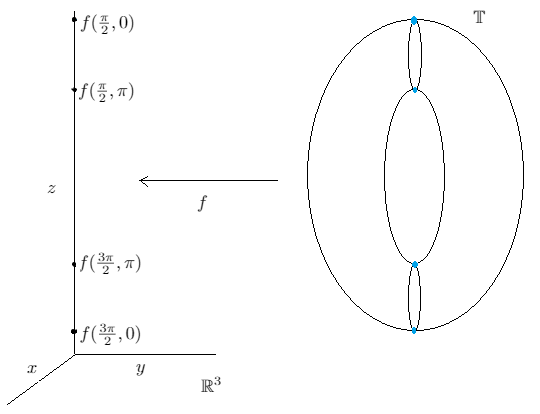
\includegraphics[scale=0.6]{ToroMorse.png}
\caption{Mapeo altura $f$ del $\mathbb{T}$ y sus valores cr\'iticos.}
\label{ToroMorse}
\end{figure}
\end{eje}

El siguiente resultado nos muestra que en el caso no degenerado, el mapeo $f$ tiene un comportamiento sencillo en un entorno del punto cr\'itco $p\in M^{m}$. M\'as a\'un, muestra como el \'indice del punto $p$ determina por completo este comportamiento.

\begin{lema}[Morse]\label{lemaMorse}
Sea $p\in M^{m}$ un punto cr\'itico no degenerado de \'indice $k$, entonces existe una carta $(U,x)$ alrededor del punto $p$ con $x(p)=0$ y tal que
\begin{equation}\label{EqLemaMorse}
f = f(p)-x_{1}^{2}-...-x_{k}^{2}+x_{k+1}^{2}+...+x_{n}^{2}                
\end{equation}
en todo $U$ y a $k$ lo llamamos el {\bfseries \'indice de Morse} de $f$ en el punto $p$.
\end{lema}

La prueba del lemma \ref{lemaMorse} [Morse] puede encontrarse en la p\'agina 6 de \cite{Matsumoto}. A partir del lema \ref{lemaMorse} se pueden obtener el siguiente corolario.  

%Sea $M^{m}$ una variedad lisa, $f:M^{m}\to\mathbb{R}$ un mapeo de Morse y $p\in M$ un punto cr\'itico no degenerado de \'indice $k$. Es posible suponer sin p\'erdida de generalidad que %$M^{m}=\mathbb{R}^{m}$, $p=0$ y $f(p)=0$ por el teorema fundamental del c\'alculo existe un entorno de $p$ tal que $f$ es de la forma 
%$$f(x)=\sum\limits_{i,j=1}^{m} h_{ij}(x)x_{i}x_{j},$$
%Es posble redefinir los mapeos $h_{ij}$ para que sean sim\'etricos para as\'i obtener expresi\'on deseada. Por \'ultimo analogamente al m\'etodo de diagonalizaci\'on de formas cuadr\'aticas %llegamos a la expresion deseada.\hfill $\square$.
%\vspace{5mm}

\begin{coro}\label{cor1}
Sea $p\in M^{m}$ un punto cr\'itico no degenerado de \'indice $k$, entonces 
\begin{itemize}
	\item $p$ es un m\'inimo si y s\'olo si $k=0$, y 
	\item $p$ es un m\'aximo si y s\'olo si $k=m$
\end{itemize}
\end{coro}
\noindent{Demostraci\'on.}\\
Al ser $p\in M^{m}$ un punto cr\'itico no degenerado, entonces aplicando el lema de Morse se tiene que en un vecindad de $p$ el mapeo $f:M^{m}\to\mathbb{R}$ es de la forma \ref{EqLemaMorse} y aplicando c\'alculo vectorial no es dif\'icil deducir que $p$ es m\'aximo cuando $k=m$, es decir, el \'indice de Morse es igual a la dimensi\'on de la variedad $M^{m}$ y que $p$ es m\'inimo cuando $k=0$ \hfill $\square$.
\vspace{5mm}

Con todo lo anterior, del ejemplo \ref{EjeMor} podemos obtener la siguiente informaci\'on de sus puntos cr\'iticos, que se detallan en el cuadro \ref{tabla0}.
\begin{table}[!ht]
\centering
\begin{tabular}{|c|c|c|c|c|}
\hline
\multicolumn{1}{|c|}{Punto Cr\'itico}     & Expresi\'on local de $f$ & \multicolumn{1}{l|}{\'Indice de Morse} & \multicolumn{1}{l|}{M\'aximo} & \multicolumn{1}{l|}{M\'inimo} \\ \hline
\multicolumn{1}{|c|}{$(\frac{\pi}{2},0)$} & $c-\theta^{2}-\phi^{2}$  & 2                                      & Si                            & No                            \\ \hline
$(\frac{\pi}{2},\pi)$                     & $c+\theta^{2}-\phi^{2}$  & 1                                      & No                            & No                            \\ \hline
$(\frac{3\pi}{2},\pi)$                    & $c+\theta^{2}-\phi^{2}$  & 1                                      & No                            & No                            \\ \hline
$(\frac{3\pi}{2},0)$                      & $c+\theta^{2}+\phi^{2}$  & 0                                      & No                            & Si                            \\ \hline
\end{tabular}
\caption{Informaci\'on de los puntos cr\'iticos del ejemplo \ref{EjeMor}.}
\label{tabla0}
\end{table}

\begin{propo}\label{PropoMor}
Sea $f:M^{m}\to\mathbb{R}$ un mapeo liso con $M^{m}$ una variedad lisa, entonces los puntos cr\'iticos no degenerados de $f$ son asilados en el conjunto de los puntos cr\'iticos.   
\end{propo}

\noindent {\bfseries Demostraci\'on.}\\
Tomemos un punto cr\'itico $p\in M$ de $f$ y $(U,x)$ una carta alrededor de $p$. Consideramos el mapeo $g:U\to\mathbb{R}^{m}$ dado como $g(p)=(\frac{\partial f}{\partial x_{1}}|_{p},...,\frac{\partial f}{\partial x_{m}}|_{p})$. Notemos que $g(p)=0$ si y s\'olo si $p$ es un punto cr\'itico de $f$. Ahora bien la matriz Jacobiana de $g$ es $\left[\frac{\partial^{2} f}{\partial x_{i}\partial x_{j}}\right]$ que es no singular en el punto $p$, es decir invertible, entonces por el teorema de funci\'on inversa $g$ es inyectiva en un vecindad de $p$ contenida en $U$ y como $g(p)=0$, entonces $p$ es el \'unico punto cr\'itico de $f$ en dicha vecindad.
\vspace{5mm}

De la proposici\'on \ref{PropoMor} se sigue inmediatamente el siguiente corolario.  

\begin{coro}\label{cor2}
Si $p\in M^{m}$ es un punto cr\'itico no degenerado de $f$, entonces existe un entorno de $p$ en el cual no hay otro punto cr\'itico de $f$. 
\end{coro}

Ahora si agregamos la hip\'otesis de que $M^{m}$ es una variedad compacta a la proposici\'on \ref{PropoMor}, entonces se tiene que los puntos cr\'iticos de $f:M^{M}\to\mathbb{R}$ son finitos [P\'agina 47, \cite{Matsumoto}].  Sin embargo en general, no es cierto que los puntos cr\'iticos de un mapeo liso sean aislados, como podemos notar en el siguiente ejemplo.

\begin{eje}\label{ejeNoDege}
Sea $f:\mathbb{R}^{2}\to\mathbb{R}^{2}$ definida como $f(x,y)=x^{2}$, entonces todos los puntos del eje $y$ son puntos cr\'iticos degenerados y forman una subvariedad de $\mathbb{R}^{2}$.
\end{eje}

Para este tipo de mapeos, donde tenemos variedades singulares es posible estudiarlos mediante la teor\'ia de Bott-Morse, que explicamos en la seccion \ref{1.3}

\section{Foliaciones de Bott-Morse}\label{1.3}

Esta secci\'on esta inspirada en los trabajos \cite{Seade1} y \cite{Seade2} realizados por Seade y Sc\'ardua. La idea de la secci\'on es generalizar el concepto de mapeo de Morse.
\vspace{5mm}

Notemos que las singularidades de los mapeos de Morse son puntos, que pueden considerarse como variedades diferenciales de dimensi\'on cero. Ahora nos interesa trabajar en el caso cuando las funciones tienen singularidades y \'estas son variedades diferenciables de dimensi\'on mayor o igual a cero. Para esto necesitamos una nueva idea de c\'omo entender que un mapeo $f:M^{m}\to\mathbb{R}$ sea no degenerado.
\vspace{5mm}

Sea $f:M^{m}\to\mathbb{R}$ un mapeo liso tal que sus puntos cr\'iticos son subvariedades ajenas de $M^{m}$. Decimos que el mapeo 
$f$ es {\bfseries no degenerado en el sentido de Bott}, si para cada $p$ en la subvariedad singular existe un disco peque\~{n}o $D_{p}$ transversal a la subvariedad singular y de dimensi\'on complementaria, tenemos que $f|_{D_{p}}$ es un punto cr\'itico no degenerado. Este concepto fue introducido en $1954$ por R. Bott en \cite{Bott}.
\vspace{5mm}

Dado $f:M^{m}\to\mathbb{R}$ un mapeo liso, denotamos al conjunto de puntos cr\'iticos de $f$ por ${\rm Sing(f)}$. 

\begin{definicion}[Bott-Morse]\label{DefBM}
Sea $M^{m}$ una variedad lisa, decimos que el mapeo liso $f:M^{m}\to\mathbb{R}$ es de Bott-Morse, si
$${\rm Sing(f)}=\bigcup_{j=1}^{t}N_{j},$$
donde $N_{j}$ es una subvariedad cerrada de $M$, $N_{j}\cap N_{i}=\emptyset$ si $j\neq i$ y el mapeo $f$ es no degenerado. 
\end{definicion}

\begin{eje}\label{ejeBM}
Consideramos un toro $\textbf{T}$ encajado en $\mathbb{R}^{3}$ y parametrizado mediante el mapeo  $X:K\to\mathbb{R}^{3}$ dado como 
$$X(\theta, \phi)= \left( sen(\phi), (r+cos(\theta))cos(\phi), (r+cos(\theta))sen(\phi) \right),$$
donde $K = [0,2\pi]\times [0,2\pi]$.
\vspace{5mm}

Ahora, consideramos el mapeo \texttt{altura}  mediante la proyecci\'on sobre el eje $x$, es decir, consideramos el mapeo 
$f:\mathbb{T}\to\mathbb{R}$ dado como 
\begin{equation}
f(\theta, \phi) = sen(\theta) 
\end{equation}

Calculemos los valores cr\'iticos de $f$, para esto calculemos el gradiente de $f$.
$$\nabla f_{(\theta,\phi)} = \left( \frac{\partial f}{\partial\theta}, \frac{\partial f}{\partial\phi} \right)|_{(\theta,\phi)} = \left( \frac{\partial sen(\theta)}{\partial\theta}, \frac{\partial sen(\theta)}{\partial\phi} \right)|_{(\theta,\phi)} = \left( cos(\theta), 0 \right)$$

Es f\'acil observar que $\nabla f = (0,0)$ si y s\'olo si $\theta\in\{\frac{\pi}{2},\frac{3\pi}{2}\}$, es decir, tenemos los puntos cr\'iticos $(\frac{\pi}{2},\phi)$ y $(\frac{3\pi}{2},\phi)$ para el mapeo $f$.   
\vspace{5mm}

Notemos que el hessiano del mapeo  $f$ es:
\begin{equation*}
Hess(f)= \left[ 
\begin{array}{cc}
-sen(\theta) & 0 \\
0            & 0
\end{array} \right]
\end{equation*}

Al calcular el hessiano de $f$ en los puntos $(\frac{\pi}{2},\phi)$ y $(\frac{3\pi}{2},\phi)$, notamos que $det(Hess(f))=0$, es decir son degenerados en el sentido de Morse, sin embargo hay que notar tambi\'en que el evaluar dichos puntos en el mapeo $X$: 
\begin{itemize}
    \item $X((\frac{\pi}{2},\phi))=(1, rcos(\phi), rsen(\phi)),$ 
    \item $X((\frac{\pi}{2},\phi))=(-1, rcos(\phi), rsen(\phi)),$
\end{itemize}
obtenemos que estos son c\'irculos singulares ajenos contenidos en $\mathbb{T}$, para esto observemos la figura \ref{ToroBottMorse} que muestra uno de los c\'irculos singulares encontrados, as\'i tenemos que {\rm Sing($f$)} son dos c\'irculos ajenos y no es dif\'icil notar que $f$ es no degenerada, as\'i podemos concluir que $f$ es de Bott-Morse.  

\begin{figure}[!ht]
\centering
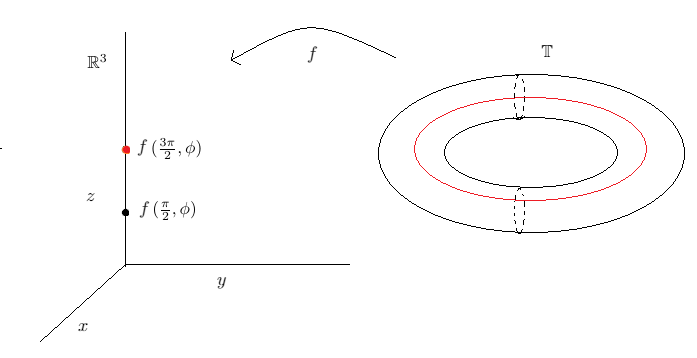
\includegraphics[scale=0.7]{ToroBottMorse.png}
\caption{C\'irculo singular del mapeo $f$ y sus valores cr\'iticos.}
\label{ToroBottMorse}
\end{figure}

\end{eje}

An\'alogamente a lo que ocurre con los mapeos de Morse, se tiene que los mapeos de Bott-Morse muestran un comportamiento sencillo en un entorno del punto $p$ en la variedad cr\'itica y muestra tambi\'en como el \'indice del punto $p$ determina por completo este comportamiento.

\begin{lema}[Bott-Morse]\label{lemaBM}
Sea $f:M^{m}\to\mathbb{R}$ un mapeo de Bott-Morse, $N^{n}$ una subvariedad singular conexa y $p\in N^{n}$. Entonces existe una carta $(U,\phi)$ de $M$ alrededor del punto $p$ con $\phi(p)=0$ y tal que
\begin{itemize}
	\item $\phi(U\cap N)= \{(x,y)\in\mathbb{R}^{n}\times\mathbb{R}^{m-n}| y=0\}$ y 
	\item $f\circ\phi^{-1}(x,y) = f(p)- y_{1}^{2}-...-y_{k}^{2}+y_{k+1}^{2}+...+y_{m-n}^{2}$
\end{itemize}
donde $\phi:U\to\mathbb{R}^{n}\times\mathbb{R}^{m-n}$ y $k\leq m-n$ es el \'indice de $f$ en $p$.
\end{lema}

La demostraci\'on puede ser consultada en el art\'iculo \cite{Banyaga} de Banyaga y Hurtubise.\\

El concepto de Bott-Morse se puede extender a una foliaci\'on $\mathcal{F}$ con singularidades, para esto denotemos como ${\rm Sing(\mathcal{F})}$ al conjunto singular de $\mathcal{F}$ y consideramos desde ahora hasta el final de esta secci\'on a $\mathcal{F}$ una foliaci\'on lisa en $M^{m}$ con singularidades de codimensi\'on uno y con $2\leq m$.\\

Las singularidades de $\mathcal{F}$ son {\bfseries singularidades de Bott-Morse} s\'i 
$${\rm Sing(\mathcal{F})}=\bigcup_{j=1}^{t}N_{j},$$
donde: 
\begin{itemize}
    \item $N_{j}$ es una subvariedad cerrada y conexa de $M$, 
    \item $N_{j}\cap N_{i}=\emptyset$ si $j\neq i$,
    \item $Codim(N_{j})\geq 2$,
    \item Para cada $p\in N_{j}$ existe un abierto $V_{p}\subset M$, donde $\mathcal{F}$ es definida por un mapeo de Bott-Morse.
\end{itemize}

Se tiene que en una singularidad de Bott-Morse $N_{j}^{n_{j}}$ existe un difeomorfismo $\varphi:V_{p}\to P\times D$ donde $P\in\mathbb{R}^{n_{j}}$ y $D\in\mathbb{R}^{m-n_{j}}$ y una foliaci\'on $\mathcal{G}$ en $D$ cuyas fibras est\'an dadas por un mapeo de Morse. As\'i $\varphi$ toma la foliaci\'on $\mathcal{F}|_{V_{p}}$ y la env\'ia a la foliaci\'on producto $P\times\mathcal{G}$.
\vspace{5mm}

En otras palabras tenemos lo siguiente:

\begin{itemize}
    \item ${\rm Sing(\mathcal{F})}\cap V_{p}=N_{j}^{n_{j}}\cap V_{p}$.
    \item $\varphi(N_{j}\cap V) = P\times \{0\}\subset\mathbb{R}^{n_{j}}\times\mathbb{R}^{m-n_{j}}$.
    \item Existen coordenadas locales 
    $$(x,y)=(x_{1},...,x_{n_{j}}, y_{1},...,y_{m-n_{j}})$$ en  $V_{p}$ tal que $N_{j}\cap V_{p}$ esta dado por  $\{y_{1},...,y_{m-n_{j}}=0\}$ y adem\'as $\mathcal{F}|_{V_{p}}$ esta dado por los niveles del mapeo  $J_{N_{j}}(\bar{x},x)=\Sigma_{j=1}^{m-n_{j}}\lambda_{j}x_{j}^{2}$, donde $\lambda=\pm 1$. 
\end{itemize}

Notemos que los dos \'ultimos puntos son consecuencias de lema \ref{lemaBM} de Bott-Morse, adem\'as el disco $\Sigma_{p}=\varphi^{-1}(x(p)\times D)$ es transversal a $N_{j}$ y es transversal a $\mathcal{F}$ fuera de $N_{j}$. La restricci\'on de $\mathcal{F}$ en $\Sigma_{p}$ es un singularidad de Morse y el \'indice de Morse es independiente del punto $p$ en la componente $N_{j}$ y de la elecci\'on del disco transversal $\Sigma_{p}$.
\vspace{5mm}

% \todo{Add definicion de tipo transversal}
Nos referimos a $\mathcal{G}(N_{j})=\mathcal{F}|_{\Sigma_{p}}$ como el tipo transversal de $\mathcal{F}$ a lo largo de $N_{j}$, la cual es una foliaci\'on de codimensi\'on uno en $\Sigma_{p}$ con una singularidad de Morse en $\{p\}=N_{j}\cap\Sigma_{p}$, a partir de esto es posible distinguir los siguientes tipos de variedades singulares $N_{j}$.

\begin{definicion}
Una componente $N_{j}\subset {\rm Sing(\mathcal{F})}$ es:
    \begin{enumerate}
        \item {\bfseries Centro} si el tipo transversal de $\mathcal{F}$ a lo largo de $N_{j}$ es un centro, es decir, el \'indice de Morse de $f|_{\Sigma_{p}}$ es $0$ o $m-n_{j}$.
        \item {\bfseries Silla} si el tipo transversal de $\mathcal{F}$ a lo largo de $N_{j}$ es una silla, es decir, el \'indice de Morse de $f|_{\Sigma_{p}}$ es diferente de  $0$ o $m-n_{j}$.
    \end{enumerate}
\end{definicion}

Por el lema de Bott-Morse en una vecindad de una componente $N_{j}$ es centro las hojas de $\mathcal{F}$ en el disco transversal $\Sigma_{p}$ son difeomorfas a $S^{(m-(n_{j}+1))}$, para esto hay que recordar que ${\rm dim}(N_{j})=n_{j}$. Para entender mejor lo anterior podemos observar la siguiente figura \ref{centro}, cuando $N_{j}$ es un variedad singular de dimensi\'on uno y $\Sigma_{p}$ es de dimensi\'on dos.

\begin{figure}[!ht]
\centering
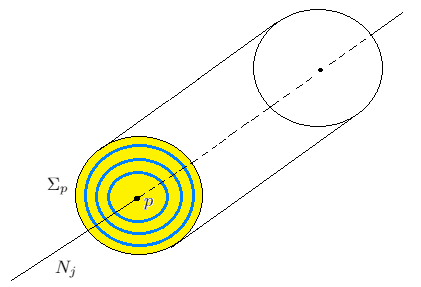
\includegraphics[scale=0.6]{centro.png}
\caption{$N_{j}$ tipo centro.}
\label{centro}
\end{figure}

De manera an\'aloga, en una vecindad de la componente $N_{j}$ silla, se tiene que las hojas de $\mathcal{F}$ en el disco transversal $\Sigma_{p}$ estan dadas de forma local por las expresiones 
$$y^{2}_{1}+...+y^{2}_{r}=y^{2}_{r+1}+...+y^{2}_{n_{j}},$$ 
donde $r$ es el \'indice de Morse de $f|_{\Sigma_{p}}$ y a dichas hojas las llamamos {\bfseries separatrices} de $\mathcal{F}$, de igual manera observemos la figura \ref{silla} para el caso cuando $N_{j}$ es un variedad singular de dimensi\'on uno y $\Sigma_{p}$ es una variedad de dimensi\'on dos.

\begin{figure}[!ht]
\centering
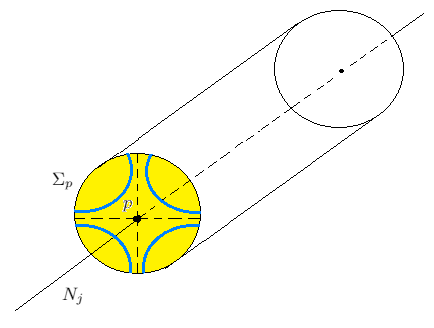
\includegraphics[scale=0.6]{silla.png}
\caption{$N_{j}$ tipo silla.}
\label{silla}
\end{figure}

Dada una componente $N_{j}$ que es silla, decimos que una {\bfseries separatriz} de $N_{j}$ es una hoja $L$ tal que su cerradura $\bar{L}$ contiene a $N_{j}$. 
\vspace{5mm}

Denotemos por ${\rm Sil(\mathcal{F})}$ a la uni\'on de $N_{j}$ que son sillas contenidos en ${\rm Sing(\mathcal{F})}$. Decimos que $\mathcal{F}$ tiene  {\bfseries silla conectadas}, si existen componentes $N_{1}$, $N_{2}\in{\rm Sil(\mathcal{F})}$ tal que $N_{1}\neq N_{2}$ y una hoja $L$ de $\mathcal{F}$ que es simult\'aneamente una separatrix de $N_{1}$ y $N_{2}$. 
\vspace{5mm}

Decimos que la foliaci\'on {\bfseries $\mathcal{F}$ es orientable}, si existe una forma diferenciable   $\omega\in\Omega^{m-1}(M^{m})$ tal que $\omega$ es no singular en $(M-{\rm Sing(\mathcal{F})})$ y $\omega|_{L}$ es una forma de volumen en cada hoja $L\in\mathcal{F}$. La elecci\'on de la forma $\omega$ es llamada {\bfseries una orientaci\'on para $\mathcal{F}$}.  
\vspace{5mm}

Tambi\'en tenemos que la foliaci\'on {\bfseries $\mathcal{F}$ es transversalmente orientable}, si existe un campo vectorial $X \in\mathcal{X} (M)$ tal que $X$ es transversal a $\mathcal{F}$ en cada punto fuera de ${\rm Sing(\mathcal{F})}$. Notemos que el campo $X$ puede tener singularidades en ${\rm Sing(\mathcal{F})}$.
\vspace{5mm}

De lo anterior, es posible obtener una definci\'on que extiende el concepto de singularidad de Bott-Morse a foliaciones singulares.
\begin{definicion}
Decimos que una foliaci\'on $\mathcal{F}$ lisa sobre $M^{m}$ de codimensi\'on uno es una {\bfseries foliaci\'on de Bott-Morse} si:
    \begin{enumerate}
        \item ${\rm Sing(\mathcal{F})}$ son singularidades de Bott-Morse.
        \item $\mathcal{F}$ es transversalmente orientable.
        \item $\mathcal{F}$ no tiene sillas conectadas en $M^{m}$.
    \end{enumerate}
\end{definicion}

Los primeros ejemplos de foliaciones con singularidades de Bott-Morse son los dados por mapeos de Bott-Morse y por productos de foliaciones de Morse definidos sobre variedades cerradas. En la secci\'on \ref{2.3} donde se introduce el concepto de foliaci\'on caracter\'istica se presentar\'a un ejemplo de foliaci\'on de Bott-Morse.\\     

Para el caso cuando la variedad $M$ es de dimensi\'on tres, que el caso que utilizaremos en este trabajo de investigaci\'on, se obtienen las siguientes posibilidades para la dimensi\'on de la variedad singular $N_{j}$ y cuando \'esta es centro o silla, las distintas posibilidades  se encuentran detalladas en el cuadro \ref{tabla1}.
\begin{table}[!ht]
\centering
\begin{tabular}{|l|l|l|c|c|}
\hline
\multirow{8}{*}{dim$(M)=3$} & \multirow{5}{*}{dim$(N_{j})=0$} & Tipo                   & \multicolumn{1}{l|}{\'Indice de Morse} & Modelo Local en $\Sigma_{p}$      \\ \cline{3-5} 
                            &                                 & \multirow{2}{*}{Centro} & cero                             & $x_{1}^{2}+x_{2}^{2}+x_{3}^{2}$  \\ \cline{4-5} 
                            &                                 &                         & tres                            & $-x_{1}^{2}-x_{2}^{2}-x_{3}^{2}$ \\ \cline{3-5} 
                            &                                 & \multirow{2}{*}{Silla} & uno                              & $-x_{1}^{2}+x_{2}^{2}+x_{3}^{2}$ \\ \cline{4-5} 
                            &                                 &                         & dos                             & $-x_{1}^{2}-x_{2}^{2}+x_{3}^{2}$ \\ \cline{2-5} 
                            & \multirow{3}{*}{dim$(N_{j})=1$} & \multirow{2}{*}{Centro} & cero                             & $x_{1}^{2}+x_{2}^{2}$            \\ \cline{4-5} 
                            &                                 &                         & dos                             & $-x_{1}^{2}-x_{2}^{2}$           \\ \cline{3-5} 
                            &                                 & Silla                  & uno                              & $-x_{1}^{2}+x_{2}^{2}$           \\ \hline
\end{tabular}
\caption{Posibles casos para $N_{j}$ cuando ${\rm dim(M)=3}$}
\label{tabla1}
\end{table}

As\'i mismo cuando la dimensi\'on de la variedad $M$ es tres, tenemos el siguiente resultado de Seade y Sc\'ardura \cite{Seade1}.
\begin{teo}\label{teoPepe}
Sea $M^{3}$ una variedad lisa, orientada, cerrada y conexa equipada con una foliaci\'on compacta de Bott-Morse, entonces 
$${\rm Sing(\mathcal{F})} = \left\{ \begin{array}{cl}
                                    \{p_{1},p_{2}\}  &  {\rm o} \\ 
                                    \{c_{1}, c_{2}\} & , 
                                    \end{array} 
                                    \right.$$
donde $p_{1}, p_{2}$ son puntos y $c_{1}, c_{2}$ son c\'irculos.
\end{teo}

La prueba del resultado anterior se puede encontrar en la p\'agina 209 de \cite{Seade1}. 

\chapter{Geometr\'ia de Poisson}\label{cap2}% Listo

Este ca\'pitulo explica la teor\'ia de la geometr\'ia de Poisson lo m\'as breve posible pero sin olvidar los aspectos m\'as importantes de ella. Para esta investigaci\'on tenemos como objetivo saber que es la foliaci\'on caracter\'istica mediante hojas simpl\'ectias inducida por una estructura de Poisson y enunciar el teorema \ref{TeoGSV} para poder construir estructuras de Poisson.\\

Para un estudio  m\'as profundo sobre la Geometr\'ia de Poisson remitimos al lector consultar la siguiente literatura \cite{Dufour} y \cite{Laurent}.

\section{Campos Multivectoriales}\label{2.1}

Sea $M^{m}$ una variedad lisa y $q$ un entero positivo. Denotaremos por $\Lambda^{q}TM$ el espacio tangente de $q-$vectores de $M$. Se tiene que $\Lambda^{q}TM$ es un haz vectorial sobre $M$, cuyas fibras sobre cada punto $p\in M$ es el espacio $\Lambda^{q}T_{p}M$, que es el producto antisim\'etrico exterior de $q$ copias del espacio tangente $T_{p}M$. \\

Tomemos un sistema local de coordenadas $(U,(x_{1},....,x_{m}))$ alrededor del punto $p\in M$. Como $\Lambda^{q}T_{p}M$ es un espacio vectorial, entonces admite una base de la forma $\{\frac{\partial}{\partial x_{i_{1}}}\wedge...\wedge\frac{\partial}{\partial x_{i_{q}}}(p) | i_{1}<...<i_{p}\}$. Es posible definir un {\bfseries $q$-campo vectorial} $\Pi$ en $M$ como una secci\'on lisa del haz $\Lambda^{q}TM$, es decir, el mapeo $\Pi:M\to\Lambda^{q}TM$ asocia a cada punto $p\in M$ con un $q-$vector $\Pi(p)\in\Lambda^{q}T_{p}M$  de forma lisa.\\

Si $(U,(x_{1},...,x_{m}))$ son coordenadas locales para $M$, entonces el $q-$vector $\Pi$ tiene la siguiente expresi\'on local:
\begin{equation}\label{Ec2.1.1}
\Pi = \sum\limits_{i_{1}<...<i_{q}}\Pi_{i_{1}...i_{q}}\frac{\partial}{\partial x_{i_{1}}}\wedge...\wedge\frac{\partial}{\partial x_{i_{q}}}
\end{equation}
donde las componentes $\Pi_{i_{1}...i_{q}}\in C^{\infty}(M)$ son antisim\'etricas y son llamadas coeficientes de $\Pi$.\\

Recordemos que los $q-$campos vectoriales $\mathcal{X}^{q}(M)$ son objetos duales a las $q-$formas diferenciales $\Omega^{q}(M)$ de una manera natural. Si $\Pi\in\mathcal{X}$, $\alpha\in\Omega^{q}(M)$ y $(U,(x_{1},...,x_{m}))$ un sistema local de coordenadas alrededor del punto $p\in M$, entonces podemos escribir.

\begin{itemize}
    \item $\Pi = \sum\limits_{i_{1}<...<i_{q}}\Pi_{i_{1}...i_{q}}\frac{\partial}{\partial x_{i_{1}}}\wedge...\wedge\frac{\partial}{\partial x_{i_{q}}}.$
    \item $\alpha = \sum\limits_{i_{1}<...<i_{q}}\alpha_{i_{1}...i_{q}}d x_{i_{1}}\wedge...\wedge d x_{i_{q}}.$
\end{itemize}

Entonces podemos definir su {\bfseries emparejamiento} como $\langle\alpha,\Pi\rangle$ como un mapeo definido como 
\begin{equation}
\langle\alpha,\Pi\rangle = \Sigma_{i_{1}<...<i_{q}}\Pi_{i_{1}...i_{q}}\alpha_{i_{1}...i_{q}}.
\end{equation}
Es f\'acil notar que la definici\'on de $\langle\alpha,\Pi\rangle$ no depende de la elecci\'on del sistema local de coordenadas.\\ 

Es particular tenemos que un $k-$campo vectorial liso en una variedad lisa $M^{m}$ puede ser considerado como un mapeo $C^{\infty}(M)$-lineal y alternante 
$$\Pi:\underbrace{\Omega^{1}(M)\times...\times\Omega^{1}(M)}_{k-veces}\to C^{\infty}(M)$$
Dado lo anterior es posible establecer la siguiente proposici\'on.

\begin{propo}\label{Propo2.1.1}
Para una variedad lisa $M^{m}$ la asignaci\'on  
\begin{equation*}
    \bar{\Pi}(f_{1},...,f_{k})=\Pi(d f_{1},...,d f_{k})
\end{equation*}
establece una correspondencia uno a uno entre los mapeos $C^{\infty}(M)$-lineales y alternantes 
\begin{equation*}
    \Pi:\underbrace{\Omega^{1}(M)\times...\times\Omega^{1}(M)}_{k-veces}\to C^{\infty}(M),
\end{equation*}
y los mapeos $\mathbb{R}$-lineales y alternantes 
\begin{equation*}
    \bar{\Pi}:\underbrace{C^{\infty}(M)\times...\times C^{\infty}(M)}_{k-veces}\to C^{\infty}(M).
\end{equation*}
Adem\'as satisfacen la regla de Leibniz en cada argumento, es decir 
\begin{equation*}
    \bar{\Pi}(f_{1},...,\bar{f}f_{i},...,f_{k})=\bar{f}(\bar{\Pi}(f_{1},...,f_{i},...,f_{k}))+f_{i}(\bar{\Pi}(f_{1},...,\bar{f},...,f_{k})).
\end{equation*}
\end{propo}
{\bfseries Demostraci\'on.}\\
Es claro que por la construcci\'on del mapeo $\bar{\Pi}$ que a todos los mapeos $\mathbb{R}-$lineales, alternantes y que satisfacen la regla de Leibniz se le puede asociar un $k-$campo vectorial.\\

Para el caso contrario s\'olo basta revisar que el valor de $\bar{\Pi}(f_{1},...,f_{k})$ en un punto $p\in M$ s\'olo depende del valor de $df_{1},...,df_{k}$ en el punto $p$; esto es equivalente a verificar que si el valor $df_{i}(x_{i})=0$ en un punto $p\in M$ para $i=1,...,k$, entonces $\bar{\Pi}(f_{1},...,f_{k})=0.$ \\

Si $df_{i}(x_{i})=0$ entonces podemos escribir de manera local a $f_{i}$ como $$f_{i}=\sum\limits_{j=1}^{k}x_{i_{j}}g_{i_{j}}+c_{i},$$
donde $x_{i_{j}},g_{i_{j}}\in C^{\infty}(M)$ son mapeos que se anulan en $p\in M$ y $c_{i}$ una constante.\\

De la regla de Leibniz se tiene que
\begin{eqnarray*}
\bar{\Pi}(f_{1},...,f_{i},...,f_{k})(p) & = &  \bar{\Pi}(f_{1},...,\sum\limits_{j=1}^{k}x_{i_{j}}g_{i_{j}}+c_{i},...,f_{k}) \\
 & = & \bar{\Pi}(f_{1},...,\sum\limits_{j=1}^{k}x_{i_{j}}g_{i_{j}},...,f_{k}) + \bar{\Pi}(f_{1},...,c_{i},...,f_{k}) \\
 & = & \bar{\Pi}(f_{1},...,\sum\limits_{j=1}^{k}g_{i_{j}},...,f_{k}) + \bar{\Pi}(f_{1},...,\sum\limits_{j=1}^{k}x_{i_{j}},...,f_{k}) \\
 & + & \bar{\Pi}(f_{1},...,c_{i},...,f_{k}) \\
 & = & \bar{\Pi}(f_{1},...,\sum\limits_{j=1}^{k}g_{i_{j}},...,f_{k}) + \bar{\Pi}(f_{1},...,\sum\limits_{j=1}^{k}x_{i_{j}},...,f_{k}) \\
 & + & c_{i}\bar{\Pi}(f_{1},...,1,...,f_{k}) \\
 & = & 0.
\end{eqnarray*}
As\'i tenemos que
\begin{eqnarray*}
\bar{\Pi}(f_{1},...,1\cdot 1,...,f_{k})  & =  & \bar{\Pi}(f_{1},...,1\cdot 1,...,f_{k}) +\bar{\Pi}(f_{1},...,1\cdot 1,...,f_{k})\\
& = & 2\bar{\Pi}(f_{1},...,1,...,f_{k}),
\end{eqnarray*}
es decir, $\bar{\Pi}(f_{1},...,1,...,f_{k})=0$.\hfill $\square$\\

Recordemos que el operador diferencial $d:\Omega^{k}(M)\to\Omega^{k+1}(M)$ juega un papel importante en la geometr\'ia diferencial. La operaci\'on que juega el papel del operador diferencial en campos multivectoriales es el corchete de Schouten-Nijenhuis, el cual lo podemos pensar c\'omo una extensi\'on del corchete de Lie.\\

Antes de continuar con la definici\'on de corchete de Schouten-Nijenhuis, vamos a explicar la siguiente notacion: Denotemos por $\xi_{i}$ a la variable $\frac{\partial}{\partial x_{i}}$; con esta notaci\'on es es posible considerar a $\xi_{i}$ como variables formales en el sentido de que no toman valores en un campo. Adem\'as forman una \'algebra antisim\'etrica, es decir se cumple que $\xi_{i}\xi_{j} = -\xi_{j}\xi_{j}$, conmutan con la variable $x_{i}$ y $\xi_{i}\xi_{j}=\frac{\partial}{\partial x_{i}}\wedge\frac{\partial}{\partial x_{j}}$ por tanto $\xi_{i}^{2} = \xi_{i}\xi_{i} = \frac{\partial}{\partial x_{i}}\wedge\frac{\partial}{\partial x_{i}} = 0$\\    

Si $\Pi$ es un $p-$campo vectorial, entonces tiene la forma de la f\'ormula \ref{Ec2.1.1} en un sistema local, entonces ahora lo consideramos como un polinomio homog\'eneo de grado $p$ en las variables formales $\xi_{i}$. Tomando la siguiente forma.

\begin{equation}
\Pi = \sum\limits_{i_{1}<...<i_{q}}\Pi_{i_{1}...i_{q}}\xi_{i_{1}}\wedge...\wedge\xi_{i_{q}}
\end{equation}

Una pregunta inmediata, es saber si es posible derivar este tipo de polinomios homog\'eneos; la respuesta es positva y para ello se aplica la siguiente formula:
$$\frac{\partial(\xi_{1_{1}}...\xi_{1_{p}})}{\partial\xi_{i_{k}}}=(-1)^{p-k}\xi_{1_{1}}...\hat{\xi_{1_{k}}}...\xi_{1_{p}},$$
donde $\hat{\xi_{1_{k}}}$ es el elemento que se omite en el producto y $1< k < p$.\\


Partiendo de lo anterior es posible enunciar la definici\'on de corchete de Schouten-Nijenhuis.

\begin{definicion}\label{DefCorSN}
Sean $M^{m}$ una variedad lisa, $A\in\mathcal{X}^{a}(M)$ y $B\in\mathcal{X}^{b}(M)$, definimos el {\bfseries corchete de Schouten-Nijenhuis} como un mapeo $[,]:\mathcal{X}^{a}\times\mathcal{X}^{b}\to\mathcal{X}^{a+b-1}$ dado como 
\begin{equation}
[A,B]_{SN}=\Sigma_{i}^{m}\frac{\partial A}{\partial\xi_{i}}\frac{\partial B}{\partial x_{i}}-(-1)^{(a-1)(b-1)}\Sigma_{i}^{m}\frac{\partial B}{\partial\xi_{i}}\frac{\partial A}{\partial x_{i}}
\end{equation}
\end{definicion}

Notemos que el corchete $[A,B]_{SN}$ es un polinomio homog\'eneo de grado $a+b-1$ en la variables formales y extra\~{n}as $\xi_{i}$, es decir, es un $(a+b-1)-$campo vectorial. Adem\'as cuando no se tenga ambig\"{u}edad sobre que corchete estamos trabajando, entonces simplemente escribiremos $[,]$ en lugar de $[,]_{SN}$

\begin{obs}
Existe muchas definiciones para el corchete de Schouten-Nijenhuis y todas son equivalentes, la raz\'on por la cual se escog\'io la definici\'on anterior es que fue posible hacer un algoritmo de dicho c\'alculo en en lenguaje de programaci\'on Python que explicamos a detalle en la secci\'on \ref{A.3} del ap\'endice.  
\end{obs}

Para tener en claro c\'omo opera el corchete de Schouten-Nijenhuis dado en la definici\'on \ref{DefCorSN} hagamos el siguiente ejemplo.

\begin{eje}
Consideremos el siguiente $2-$campo vectorial  
\begin{eqnarray*}
     \Pi & = & \left(-x_{3} \frac{\partial}{\partial x_{1}}\wedge\frac{\partial}{\partial x_{2}} - x_{2}\frac{\partial}{\partial x_{1}}\wedge\frac{\partial}{\partial x_{3}} + x_{1}\frac{\partial}{\partial x_{2}}\wedge\frac{\partial}{\partial x_{3}}\right).\\
         & = & -x_{3}\xi_{1}\xi_{2} - x_{2}\xi_{1}\xi_{3} + x_{1}\xi_{2}\xi_{3}.
\end{eqnarray*}
Ahora calculemos el corchete de Schouten-Nijenhuis de el mismo, es decir:
    \begin{eqnarray*}
            [\Pi,\Pi] & = & 2\left(\frac{\partial\Pi}{\partial\xi_{1}}\wedge\frac{\partial\Pi}{\partial x_{1}} 
                            +\frac{\partial\Pi}{\partial\xi_{2}}\wedge\frac{\partial\Pi}{\partial x_{2}} + \frac{\partial\Pi}{\partial\xi_{3}}\wedge\frac{\partial\Pi}{\partial x_{3}} \right)\\
                      & = & 2(-(x_{3}\xi_{2}+x_{2}\xi_{3})(\xi_{2}\xi_{3})\\ 
                      & + & 2(x_{3}\xi_{1} + x_{1}\xi_{3})(-\xi_{1}\xi_{3})\\ 
                      & + & 2(x_{2}\xi_{1} - x_{1}\xi_{2})(-\xi_{1}\xi_{2})\\
                      & = & 0.
    \end{eqnarray*}
\end{eje}

Despu\'es de entender como funciona el corchete de Schouten-Nijenhuis, este cumple con las siguientes propiedades. La prueba de esto se puede encontrar en [P\'agina 28, \cite{Dufour}]. 

\begin{teo}[Schouten-Nijenhuis]
El corchete definido en la definici\'on \ref{DefCorSN} satisface las siguientes propiedades:
\begin{description}
    \item [(i)]   {\bfseries Anticonmiutatividad:} 
        \begin{description}
            \item $[A,B]=-(-1)^{(a-1)(b-1)[B,A]}.$
        \end{description}
    \item [(ii)]  {\bfseries Casi Regla de Leibniz:} 
        \begin{description}
            \item $[A, B\wedge C]= [A,B]\wedge C + (-1)^{b(a-1)}B\wedge [A,C].$
            \item $[A\wedge B, C]= A\wedge[B,C] + (-1)^{b(c-1)}[A,C]\wedge B$.
        \end{description}
    \item [(iii)] {\bfseries Casi identidad de Jacobi:} 
        \begin{description}
            \item $(-1)^{(a-1)(c-1)}[A,[B,C]]+(-1)^{(b-1)(a-1)}[B,[C,A]]+(-1)^{(c-1)(b-1)}[C,[A,B]]=0.$
        \end{description}
\end{description}
Para toda $A\in\mathcal{X}^{a}(M)$, $B\in\mathcal{X}^{b}(M)$ y $C\in\mathcal{X}^{c}(M)$.\hfill $\square$
\end{teo}

Para terminar esta secci\'on definimos el producto interior de una $1-$forma $\alpha$ con el $k-$vector $\pi$ como el $(k-1)-$vector $i_{\alpha}\pi$ definido por  
$$i_{\alpha}\pi(\alpha_{1},...,\alpha_{k-1})=\pi(\alpha,\alpha_{1},...,\alpha_{k-1}),$$
donde $\alpha_{i}\in\Omega^{1}(M)$. 

\section{Variedades de Poisson}\label{2.2}
\begin{definicion}\label{DefPoi}
Un {\bfseries corchete de Poisson} en una variedad diferenciable $M^{m}$, es una operaci\'on binaria $$\{,\}:C^{\infty}(M)\times C^{\infty}(M)\to C^{\infty}(M),$$ que satisface 

\begin{description}
    \item [(i)]   {\bfseries $\mathbb{R}$-lineal} $\{f,ag+bh\}=\{f,ag\}+\{f,bh\}.$ 
    \item [(ii)]  {\bfseries Antisimetr\'ia} $\{f,g\}=-\{g,f\}.$ 
    \item [(iii)] {\bfseries Identidad de Jacobi} $\{f,\{g,h\}\}+=\{g,\{h,f\}\}+\{h,\{f,g\}\}=0,$
    \item [(iv)]  {\bfseries Identidad de Leibniz} $\{f,g\cdot h\}=g\cdot\{f,h\}+\{f,g\}\cdot h.$
\end{description}
para $f,g,h\in C^{\infty}(M)$ y $a,b\in\mathbb{R}$. 
\end{definicion}

Al par $(M,\{,\})$ lo llamamos una {\bfseries variedad de Poisson} y notemos que las propiedades (i)-(iii) de la definici\'on \ref{DefPoi} nos dicen que el par $(C^{\infty}(M),\{,\})$ es un \'algebra de Lie. Tambi\'en  de la definici\'on \ref{DefPoi} es inmediato el siguiente lema.   

\begin{lema}\label{lema2.2.1}
Para cualquier $f\in C^{\infty}(M)$ se cumple que $\{1,f\}=0$.
\end{lema}
{\bfseries Dem.}\\
Para la demostraci\'on s\'olo basta utilizar la identidad de Leibniz
\begin{eqnarray*}
\{1,f\} & = & \{1\cdot 1,f\}\\
        & = & 1\cdot\{1,f,\}+\{1,f\}\cdot 1\\
        & = & 2\cdot\{1,f\}.  
\end{eqnarray*}
\hfill $\square$

Cualquier variedad lisa $M^{n}$ es una variedad de Poisson, dotando a $M$ con el {\bfseries corchete trivial de Poisson}, el cual est\'a dado como $\{f,g\}=0$ para toda $f,g\in C^{\infty}(M)$. A continuaci\'on procedemos a estudiar ejemplos m\'as elaborados.\\

Un ejemplo inmediato de una variedad de Poisson, es definiendo el {\bfseries corchete de Poisson can\'onico} en $\mathbb{R}^{2n}$.

\begin{eje}\label{eje2.2.1}
Sea $\mathbb{R}^{2n}$ con coordenadas locales $(q^{1},...,q^{n},p_{1},...,p_{n})$ y sea 
\begin{equation}
\{f,g\} = \Sigma_{i=1}^{n} \left( \frac{\partial f}{\partial p_{i}} \cdot \frac{\partial g}{\partial q^{i}}-\frac{\partial f}{\partial q^{i}} \cdot \frac{\partial g}{\partial p_{i}} \right).      
\end{equation}
\end{eje}

Otro ejemplo interesante ser\'ia.

\begin{eje}\label{eje2.2.2}
Sea $(\mathfrak{g},[,]_{\mathfrak{g}})$ un \'algebra de Lie finita, si $f:\mathfrak{g}^{*}\to\mathbb{R}$ es un mapeo liso y tomamos $\xi\in\mathfrak{g}^{*}$, donde $\mathfrak{g}^{*}$ denota el \'algebra dual de $\mathfrak{g}$, entonces se tiene que la diferencial $d_{\xi}f:T_{\xi}\mathfrak{g}^{*}\to\mathbb{R}$ puede ser vista como un elemento de $\mathfrak{g}\cong(\mathfrak{g}^{*})^{*}$.\\

As\'i podemos definir un corchete de Poisson en $\mathfrak{g}^{*}$ como $$\{f,g\}(\xi):=\xi([d_{\xi}f,d_{\xi}g]_{g}).$$
Por lo tanto el par $(\mathfrak{g}^{*},\{,\})$ es una variedad de Poisson.
\end{eje}

Un corchete dado como en el ejemplo \ref{eje2.2.2} es llamado {\bfseries corchete lineal de Poisson}, pues dado un espacio vectorial $V$ con un corchete de Poisson $\{,\}_{V}$ con la propiedad de que el corchete de dos funciones lineales es una funci\'on lineal, entonces se tiene que $V^{*}$ tiene una estructura natural de \'algebra de Lie. Adem\'as $\{,\}_{V}$ coincide con el corchete de Poisson de $V^{*}$ definido como en el ejemplo \ref{eje2.2.2}.

\begin{definicion}\label{DefMapPoi}
Dadas dos variedades de Poisson $(M_{1},\{,\}_{M_{1}})$ y $(M_{2},\{,\}_{M_{2}})$, decimos que un mapeo diferenciable $\phi:M_{1}\to M_{2}$ es un {\bfseries mapeo de Poisson}, si se cumple que 
$$\{f\circ\phi,g\circ\phi\}_{M_{1}}=\{f,g\}_{M_{2}}\circ\phi$$ 
para toda $f,g\in C^{\infty}(M_{2})$.
\end{definicion}

Para observar ejemplos de mapeos de Poisson, retomaremos los ejemplos dados anteriormente.

\begin{eje}\label{eje2.2.3}
Tomemos la variedad de Poisson dada en el ejemplo \ref{eje2.2.1} y el siguiente mapeo 
$\phi:\mathbb{R}^{2n}\to\mathbb{R}^{2m}$ definido como 
$$\phi(q^{1},...,q^{n},p_{1},...,p_{n})=(q^{1},...,q^{m},p_{1},...,p_{m}),$$ 
con $n\geq m$. Entonces $\phi$ es un mapeo de Poisson, para probarlo veamos que se cumple la propiedad pedida en la definici\'on \ref{DefMapPoi}
\begin{eqnarray*}
    \{f\circ\phi,g\circ\phi\}_{\mathbb{R}^{2m}} & = &\Sigma_{i=1}^{n} \left( \frac{\partial (f\circ\phi)}{\partial p_{i}} \cdot \frac{\partial (g\circ\phi)}{\partial q^{i}}-\frac{\partial (f\circ\phi)}{\partial q^{i}} \cdot \frac{\partial (g\circ\phi)}{\partial p_{i}} \right) \\
                              & = & \Sigma_{i=1}^{n} \left( \Sigma_{j} \frac{\partial f(\phi)}{\partial\phi_{j}} \cdot \frac{\phi_{j}}{p_{i}} \cdot \frac{\partial g(\phi)}{\partial \phi_{j}} \cdot \frac{\phi_{j}}{\partial q^{i}} \right) \\
                              & - & \Sigma_{i=1}^{n} \left( \Sigma_{j} \frac{\partial f(\phi)}{\partial\phi_{j}} \cdot \frac{\phi_{j}}{\partial q^{i}} \cdot \frac{\partial g(\phi)}{\phi_{j}} \cdot \frac{\phi_{j}}{\partial p_{i}} \right) \\
                              & = &\Sigma_{i=1}^{n}\left( \frac{\partial f(\phi)}{p_{i}} \cdot \frac{\partial g(\phi)}{\partial q^{i}}-\frac{\partial f(\phi)}{\partial q^{i}} \cdot \frac{\partial g(\phi)}{\partial p_{i}} \right) \\
                              & = &\left( \Sigma_{i=1}^{n} \left( \frac{\partial f}{p_{i}} \cdot \frac{\partial g}{\partial q^{i}}-\frac{\partial f}{\partial q^{i}} \cdot \frac{\partial g}{\partial p_{i}}\right)\right)\circ\phi\\
                              & = & \{ f,g \}_{\mathbb{R}^{2n}}\circ\phi.
\end{eqnarray*}
Por lo tanto $\phi$ es una mapeo de Poisson.
\end{eje}

\begin{eje}\label{eje4}
Ahora consideremos la variedad de Poisson dada en el ejemplo \ref{eje2.2.2} y un homormofismo de \'algebras de Lie $\Phi:\mathfrak{g}\to\bar{\mathfrak{g}}$, entonces el homormorfismo transpuesto $\Phi^{*}:\bar{\mathfrak{g}}^{*}\to\mathfrak{g}^{*}$ es un mapeo de Poisson. Para mostrar esta afirmaci\'on tomemos $\xi\in\bar{\mathfrak{g}}^{*}$ veamos que se cumple con la condici\'on pedida
en la definici\'on \ref{DefMapPoi}, 
\begin{eqnarray*}
    \{f\circ\Phi^{*},g\circ\Phi^{*}\}_{\bar{\mathfrak{g}}^{*}}(\xi) & = & \xi([d_{\xi}(f\circ\Phi^{*}),d_{\xi}(g\circ\Phi^{*})]_{\bar{\mathfrak{g}}}) \\
                                                              & = & \xi([(\Phi(d_{\Phi^{*}(\xi)}f),\Phi(d_{\Phi^{*}(\xi)}g)]_{\bar{\mathfrak{g}}})\\
                                                              & = & \xi(\Phi([d_{\Phi^{*}(\xi)}f,d_{\Phi^{*}(\xi)}g]_{\mathfrak{g}})\\
                                                              & = & \Phi^{*}(\xi)([d_{\Phi^{*}(\xi)}f,d_{\Phi^{*}(\xi)}g]_{\mathfrak{g}})\\
                                                              & = & \{f,g\}_{{\mathfrak{g}^{*}}}\circ\Phi^{*}(\xi)
\end{eqnarray*}
Por lo cual el mapeo $\Phi^{*}$ es un mapeo de Poisson.
\end{eje}

Ahora veremos como se ve la expresi\'on local del corchete de Poisson mediante la siguiente proposici\'on.

\begin{propo}\label{propo1}
Sea $(M,\{,\})$ una variedad de Poisson de dimensi\'on $n$, si $(U,\varphi)$ es una carta de $M$ con $\varphi=(x_{1},...,x_{n})$, entonces para cualquier $f,g\in C^{\infty}(M)$ se tiene que el corchete de Poisson de $M$ en coordenadas locales se ve como:
$$\{f,g\}|_{U}=\sum_{i,j=1}^{n=1}\{x_{i},x_{j}\}\frac{\partial f}{\partial x_{i}}\frac{\partial g}{\partial x_{j}}.$$
\end{propo}
{\bfseries Demostraci\'on.}\\
Se tiene por el lema \ref{lema2.2.1} que $\{c,f\}=c\{1,f\}=0$ para toda $c\in\mathbb{R}$, ahora s\'olo basta probar lo anterior para un mapeo liso. Sea $f\in C^{\infty}(U)$ y tomemos su desarrollo de Taylor de orden dos alrededor del punto $\bar{x}\in U$:
$$f(x)=f(\bar{x})+\sum_{i=1}^{m}\frac{\partial f}{\partial x_{i}}(\bar{x})(x_{i}-\bar{x_{i}}) + \sum_{i,j=1}^{m}F_{ij(x)}(x_{i}-\bar{x_{i}})(x_{j}-\bar{x_{j}}),$$
para algunas funciones lisas $F_{ij}\in C^{\infty}(U)$, entonces para $f,g\in C^{\infty}(M)$ el corchete de Poisson esta dado por:
\begin{eqnarray*}
\{f,g\}(x) & = & \{f(\bar{x})+\Sigma_{i=1}^{m} \frac{\partial f}{\partial x_{i}}(\bar{x})(x_{i}-\bar{x_{i}}) \\ 
           & + & O(2), g(\bar{x})+\Sigma_{i=1}^{m} \frac{\partial g}{\partial x_{i}}(\bar{x})(x_{i}-\bar{x_{i}}) + O(2)\} \\
           & = & \Sigma_{i,j=1}^{m}\frac{\partial f}{\partial x_{i}}(\bar{x})\frac{\partial g}{\partial x_{j}} (\bar{x}) \{x_{i},x_{j}\}(x) + \Sigma_{i=1}^{m} H_{i}(x)(x_{i}-\bar{x}_{i})
\end{eqnarray*}
para algunas funciones lisas $H_{i}\in C^{\infty}(U)$. Por lo tanto, en $x=\bar{x}$ se tiene que 
$$\{f,g\}(\bar{x})= \sum_{i,j=1}^{m}\frac{\partial f}{\partial x_{i}}(\bar{x})\frac{\partial g}{\partial x_{j}}(\bar{x})\{x_{i},x_{j}\}(\bar{x})$$ 
donde $\bar{x}$ era un punto arbitrario en $U$. \hfill $\square$\\

Tenemos que en una variedad de Poisson $(M,\{,\})$ podemos restringir el corchete de Poisson a un conjunto $U\subset M$ abierto obteniendo como resultado un nuevo corchete $\{,\}_{U}$ tal que para cualquier $f,g\in C^{\infty}(M)$ se cumple que $\{f,g\}|_{U}=\{f|_{U},g|_{U}\}_{U}$. Por esta raz\'on no haremos distinci\'on entre $\{,\}$ y $\{,\}_{U}$, tal y como se hizo en la proposici\'on \ref{propo1}.\\  

La propiedad (iv) de la definici\'on \ref{DefPoi} nos permite definir para cada funci\'on $H\in C^{\infty}(M)$ un campo vectorial $X_{H}\in\mathcal{X}(M)$ definido como: 
\begin{equation}\label{DefHam}
X_{H}(f):=\{H,f\}
\end{equation} 
para toda $f\in C^{\infty}(M)$. El campo vectorial $X_{H}$ es llamado {\bfseries campo Hamiltoniano} con mapeo Hamiltoniano $H$. Una mapeo $f$ es llamado una {\bfseries integral primera} de un campo vectorial $X$, si $f$ es constante a lo largo cada \'orbita de $X$. Se puede probar que $f$ es integral primera si y s\'olo s\'i $X(f)=0$.\\   

Dadas integrales primeras es posible encontrar nuevas integrales primeras, esto es un resultado de Poisson que puede ser consultado en \cite{Poisson}.  

\begin{propo}\label{PropoPoisson}[Poisson]
Si $g$ y $h$ son integrales primeras de un campo vectorial hamiltaniano  $X_{f}$ es una variedad de Poisson $(M, \{,\})$, entonces $\{g, h\}$ es una integral primera.
\end{propo}
{\bfseries Demostraci\'on.}\\
Sean $g$ y $h$ primeras integrales de un campo vectorial $X_{f}$, entonces se tiene que 
\begin{itemize}
    \item $X_{f}(g)=\{X_{f},g\}=0$,
    \item $X_{f}(h)=\{X_{f},h\}=0.$
\end{itemize}
Aplicando la identidad de Jacobi para $h$, $g$ y $X_{f}$ tenemos 
$$\{h,\{X_{f},g\}\}+\{X_{f},\{g,h,\}\}+\{g,\{h,X_{f}\}=0,$$
y se sigue que $\{X_{f},\{g,h,\}\}=0$. Por lo tanto $\{g,h\}$ es una integral primera. \hfill $\square.$\\

Otra consecuencia inmediata de la definici\'on \ref{DefPoi} es que la asignaci\'on de un mapeo liso $f\in C^{\infty}(M)$ a un campo vectorial $X_{f}\in\mathcal{X}(M)$ es morfismo de \'algebras de Lie y la siguiente proposici\'on.

\begin{propo}\label{propoHamilto}
Sea $(M;\{,\})$ una variedad de Poisson, entonces para cada $f,g\in C^{\infty}(M)$ se tiene que $X_{\{f,g\}}=[X_{f},x_{g}].$
\end{propo}
\noindent{\bfseries Demostraci\'on.}\\
Para cualquier $f,g,h\in C^{\infty}(M)$ calculamos:
\begin{eqnarray*}
X_{\{f,g\}}(h) & = & \{\{f,g\},h\} = \{\{f,h\},g\} + \{f,\{g,h\}\} = \{f,\{g,h\}\} - \{g,\{f,h\}\} \\
               & = & X_{f}(X_{g}(h)) - X_{g}(X_{f}(h)) = [X_{f},X_{g}](h).
\end{eqnarray*}
\hfill $\square$\\

Se dice que una mapeo $f\in C^{\infty}(M)$ es un {\bfseries mapeo Casimir} si cumple que $\{f,g\}=0$ para toda $g\in C^{\infty}(M)$.\\

Dada una variedad de Poisson $(M^{m},\{,\})$ es posible definir un $2-$campo vectorial $\pi\in\mathcal{X}^{2}(M)$ mediante la asignaci\'on: 
\begin{equation}\label{BivePois}
\pi(df,dg)=\{f,g\}
\end{equation}
donde $f,g\in C^{\infty}(M)$ y $d:\Omega^{*}(M)\to\Omega^{*}(M)$ es la derivada exterior.\\
 
De manera inversa tambi\'en es posible lograrlo mediante la proposici\'on \ref{Propo2.1.1}. A saber, si tenemos un $2-$campo vectorial $\pi\in\mathcal{X}^{2}(M)$ es posible definir un corchete de mapeos lisos como en la ecuaci\'on \ref{BivePois}; es claro notar que dicho corchete cumple con la propiedades (i),(ii) y (iv) de la definici\'on \ref{DefPoi}, es decir, un bivector $\pi$ en general no cumple con la identidad de Jacobi.\\

Notemos que al calcular el corchete de Schouten-Nienhuis del $2-$campo vectorial $\pi$ consigo mismo, obtenemos que la identidad de Jacobi para el corchete $\{,\}$ es equivalente a que $[\pi,\pi]=0$, dando pie a la siguiente proposici\'on. 
\begin{propo}\label{PropoBivPoi}
Sea $(M, \{,\})$ una variedad de Poisson, entonces el $2-$ campo vectorial $\pi$ asociado a $\{,\}$ por la ecuaci\'on \ref{BivePois} satisface:
\begin{equation}\label{CSN=0}
[\pi, \pi]=0.
\end{equation}
Rec\'iprocamente, cada $2-$campo vectorial $\pi$ que satisfaga la ecuaci\'on \ref{CSN=0} define un corchete de Poisson en $C^{\infty}(M)$ por $\{f,g\}:=\pi(df,dg)$.   
\end{propo}
Un $2-$campo vectorial $\pi\in\mathcal{X}^{2}(M)$ que cumple con la condici\'on dada en la proposici\'on \ref{PropoBivPoi} es llamada una {\bfseries estructura de Poisson} sobre $M^{m}$ y al par $(M, \pi)$ lo llamamos una variedad de Poisson. De ahora en adelante s\'olo escribiremos que $M^{m}$ es una variedad Poisson, pasando por alto el corchete o la estructura de Poisson.\\

Si consideramos $(U,(x_{1},...,x_{m}))$ coordenadas locales para $M$ alrededor del punto $p\in M$, entonces de la ecuaci\'on \ref{Ec2.1.1} el $2-$campo vectorial $\pi$ tiene la siguiente expresi\'on local:
\begin{equation}\label{Ec2.2.1}
\pi|_{U} = \sum_{i<j}\pi_{ij}(p)\frac{\partial}{\partial x_{i}}\wedge\frac{\partial}{\partial x_{j}},
\end{equation}
donde $\pi_{ij}(p)=\{x_{i},x_{j}\}(p)$.\\

De igual manera considerando $(U,(x_{1},...,x_{m}))$ coordenadas locales para $M$ alrededor del punto $p\in M$, se tiene que la ecuaci\'on \ref{CSN=0} tiene la siguiente expresi\'on local:
\begin{equation}\label{PoiRel}
\sum_{h=1}^{m} \left( \pi_{hi}\frac{\partial\pi_{jk}}{\partial x_{h}} + \pi_{hj}\frac{\partial\pi_{ki}}{\partial x_{h}} + \pi_{hi}\frac{\partial\pi_{ij}}{\partial x_{h}} \right) = 0
\end{equation}
Notemos que en la ecuaci\'on \ref{PoiRel} es un sistema de ecuaciones en derivadas parciales no lineales, donde tenemos $\dbinom{m}{3}$ ecuaciones con $\dbinom{m}{2}$ funciones variables $\pi_{ij}$. Es por esta raz\'on que el estudio de las estructuras de Poisson en una variedad dada, incluso localmente, es un tema no trivial y dif\'icil.\\

Ahora notemos que dado un $2-$campo vectorial $\pi\in\mathcal{X}^{2}(M)$ este define un mapeo $\pi^{\#}:\Omega^{1}(M)\to\mathcal{X}(M)$ definido como $\pi^{\#}(\alpha)=i_{\alpha}\pi$ con $\alpha\in\Omega^{1}(M)$, dado que el mapeo producto interior es una operaci\'on puntual, este mapeo es inducido por un mapeo de haces lisos que denotaremos con el mismo s\'imbolo $\pi^{\#}:TM\to T^{*}M$ y que en cada punto $p\in M$ esta dado como 
\[\begin{array}{ccrl}
\pi_{p}^{\#} :& T_{p}^{*}M  & \to & T_{p}M \\
          & \alpha & \mapsto & i_{\alpha}\pi_{p}.
\end{array}\]
Al mapeo $\pi^{\#}$ lo llamaremos el {\bfseries mapeo ancla de $\pi$}. Un $2-$campo vectorial $\pi$ es llamado {\bfseries no degenerado en el punto $p\in M$}, si el mapeo $\pi_{p}^{\#}:T_{p}^{*}M\to T_{p}M$ es un isomorfismo de fibrados vectoriales y decimos que $\pi$ es {\bfseries no degenerado} si es no degenerado en cada punto $p\in M$.  
  
\begin{lema}\label{lema2.3.1}
Existe una correspondencia uno a uno de los $2-$campos vectoriales no degenerados $\pi\in\mathcal{X}^{2}(M)$ con las $2-$formas no degeneradas $\omega\in\Omega^{2}(M)$.  
\end{lema} 
 
{\bfseries Demostraci\'on.}\\
Dada una $2-$forma no degenerada $\omega\in\Omega^{2}(M)$, podemos determinar el mapeo $\omega^{\flat}:T M\to T^{*}M$ tal que en cada punto $p\in M$ esta dado como:    
\[\begin{array}{ccrl}
\omega_{p}^{\flat} :& T_{p}M  & \to & T_{p}^{*}M \\
          & v & \mapsto & i_{v}\omega_{p},
\end{array}\]
donde una $2-$forma $\omega$ es {no degenerada en $p\in M$}, si el mapeo $\omega_{p}^{\flat}:T_{p} M\to T_{p}M$ es un isomorfismo de fibrados vectoriales y decimos que el mapeo $\omega$ es {\bfseries no degenerado} si es no degenerado en cada punto $p\in M$.\\

Ahora tomamos el mapeo biyectivo $\pi^{\#}:T^{*}M\to TM$ y notamos que $\pi^{\#}=(\omega^{\flat})^{-1}$ y que $\omega^{\flat}=(\pi^{\#})^{-1}$.  \hfill $\square$.

\begin{definicion}\label{DefSimp}
Sea $M^{m}$ una variedad lisa, entonces decimos que una {\bfseries estructura simpl\'ectica para $M^{m}$} es una $2-$forma cerrada y no degenerada $\omega\in\Omega^{2}(M)$, donde $\omega$ es {\bfseries cerrada} si se cumple que $d\omega=0$. Al par $(M^{m}, \omega)$ lo llamamos una {\bfseries variedad simpl\'ectica}.
\end{definicion}

Las primeras propiedades que se obtienen de una variedad simpl\'ectica, es que la dimensi\'on de la variedad $M^{m}$ es siempre es par, es decir, $m=2n$. Adem\'as se cumple que si $\omega$ es una estructura simpl\'ectica para $M^{m}$ entonces $\underbrace{\omega\wedge...\wedge\omega}_{m-veces}\neq0$ y viceversa.

\begin{propo}\label{propo2.3.1}
Existe una correspondencia uno a uno entre las estructuras de Poisson no degeneradas y las estructuras simpl\'ecticas en una variedad $M^{m}$.   
\end{propo}

{\bfseries Demostraci\'on.}\\
S\'olo basta recordar que por la proposici\'on \ref{Propo2.1.1} existe una correspondencia uno a uno entre los $2-$campos vectoriales y las estructuras de Poisson en una variedad $M^{m}$ y concluimos la prueba utilizando el lema \ref{lema2.3.1}. \hfill $\square$. \\ 

Recordemos que de la ecuaci\'on \ref{Ec2.2.1} un $2-$campo vectorial tiene la siguiente expresi\'on local 
$$\pi|_{U} = \sum_{i<j}\pi_{ij}(p)\frac{\partial}{\partial x_{i}}\wedge\frac{\partial}{\partial x_{j}}$$      
y si adem\'as $\pi$ es no degenerado en un punto $p\in M$, entonces tenemos que la matriz $[\pi_{ij}(p)]$ es invertible; as\'i pues, tenemos que la expresi\'on local de la estructura simpl\'ectica es 
\begin{equation}
\omega|_{U}=\sum_{i<j}\omega_{ij}d x_{i}\wedge d x_{j},
\end{equation}
donde $\omega_{ij}=(\pi_{ij}(p))^{-1}$.\\

Terminaremos la secci\'on dando un ejemplo de una variedad simpl\'ectica.

\begin{eje}\label{ejeSim}
El ejemplo est\'andar para una variedad simpl\'ectica es tomar $\mathbb{R}^{2n}$ con coordenadas locales $(q^{1},...,q^{n},p_{1},...,p_{n})$ y considerar la siguiente estructura simpl\'ectica  
\begin{equation}
\omega=\sum_{i=1}^{n}d q_{i}\wedge d p_{i}.
\end{equation}
A lo anterior lo llamamos la {\bfseries estructura simpl\'ectica can\'onica} de $\mathbb{R}^{2n}$.  
\end{eje}

Cabe mencionar que la estructura de Poisson dada en \ref{eje2.2.1} es no degenerada y su estructura simpl\'ectica correspondiente coincide con la estructura simplectica dade en \ref{ejeSim}.

\section{Foliaci\'on Simpl\'ectica de una Variedad de Poisson}\label{2.3}

Si consideramos $(U,(x_{1},...x_{m}))$ coordenadas locales para $M^{m}$ en un punto $p\in M$ se tiene que el mapeo $\pi^{\#}_{p}$ tiene la siguiente expresi\'on local 
\begin{eqnarray*}
\pi_{p}^{\#}(\sum_{i=1}^{m}a_{i}dx_{i}) & = & \sum_{ij}\{x_{i},x_{j}\}a_{i}\frac{\partial}{\partial x_{j}}\\
                                        & = & \sum_{ij}\pi_{ij}\frac{\partial}{\partial x_{j}} 
\end{eqnarray*}
As\'i obtenemos que el mapeo $\pi^{\#}$ esta dado por la matriz $[\pi_{ij}]$ en las bases lineales $\{dx_{1},...,dx_{m}\}$ y $\{\frac{\partial}{\partial x_{1}},...,\frac{\partial}{\partial x_{m}}\}$.\\

Dado el mapeo $\pi^{\#}$ definimos
\begin{equation}\label{EqEspaCarac}
C_{p}={\rm Ima(\pi^{\#}_{p})}
\end{equation}
al espacio $C_{p}$ y lo llamaremos el {\bfseries espacio caracter\'istico de $p\in M$} de la estructura de Poisson $\pi$. \\

A la dimensi\'on de $C_{p}$ lo llamamos el {\bfseries rango de $\pi$ en $p\in M$}, de la antisimetr\'ia del mapeo $\pi^{\#}$ se tiene que el rango de $\pi$ en cada punto $p\in M$ es par y en general el rango de $\pi$ puede variar en cada punto.\\

Un punto $p_{0}\in M$ es llamado un {\bfseries punto regular de $\pi$}, si existe una vecindad $U_{p_{0}}$ tal que el rango de $\pi$ en $p$ y el rango de $\pi$ en $p_{0}$ coinciden para todo $p\in U_{p_{0}}$. En caso contrario diremos que $p_{0}$ es un {\bfseries punto singular de $\pi$}.

\begin{definicion}
Decimos que una estructura de Poisson $\pi\in\mathcal{X}^{2}(M)$ es una {\bfseries estructura regular}, si el rango de $\pi$ es constante en toda $M$.  
\end{definicion}

El espacio caracter\'istico de $\pi^{\#}$ una distribuci\'on regular lisa $C=\{C_{p}:p\in M\}$ est\'a generada por campos vectoriales de la forma $X_{f}=\pi^{\#}(df)$, es decir, por los campos vectoriales hamiltonianos. Esta distribuci\'on es llamada la {\bfseries distribuci\'on caracter\'istica de una estructura de Poisson}.\\

Si la estructura de Poisson $\pi$ es regular, entonces decimos que la distribuci\'on caracter\'istica es {\bfseries regular}, si $\pi$ no es regular, entonces decimos que la distribuci\'on caracter\'istica es {\bfseries singular}.\\

La distribuci\'on caracter\'istica resulta ser una distribuci\'on integrable. Por tanto, toda variedad de Poisson $M$ es foliada por hojas $L$ de la distribuci\'on caractater\'istica. M\'as a\'un la estructura de Poisson de $M$ induce la estructura simpl\'ectica en las hojas $L$. Probaremos lo anterior para ambos casos.\\

Para el primer caso donde consideramos una estructura de Poisson regular $\pi$, probaremos el siguiente teorema.
\begin{teo}
La distribuci\'on caracter\'istica $C_{p}$ inducida por un $2-$campo vectorial $\pi$ definido en $M$ es integrable y la estructura de Poisson $\pi$ induce estructuras simpl\'ecticas en sus hojas.  
\end{teo}
{\bfseries Demostraci\'on.}\\
La distribuci\'on $C$ es involutiva, ya que es generada por campos vectoriales hamiltoniamos, hay que recordar que 
$$C_{p}=\pi^{\#}_{p}(df)=X_{f}(p)={\rm Span}(\{X_{f}(p):f\in C^{\infty}(M)\})$$ 
y por la proposici\'on \ref{PropoPoisson} se tiene que el corchete de Lie de campos hamiltonianos es hamiltoniano, entonces por el teorema de Frobenius \ref{TeoFro} se tiene que la distribuci\'on en integrable, es decir, es la distribuci\'on tangente de una foliaci\'on regular.\\

Sea $L_{p}$ una hoja para alg\'un $p\in M$ entonces tenemos que $C_{p}\subset T_{p}L_{p}$ y la estructura de Poisson inducida $\pi|_{L_{p}}$ satisface para toda $\alpha\in T^{*}_{p}L_{p}$ 
$$\pi^{\#}(\alpha)=\pi|_{L_{p}}(\alpha|_{L_{p}}).$$
Esto muestra que $C_{p}=T_{p}L_{p}$, por lo tanto $\pi|_{L_{p}}$ es no degenerada, es decir, es simpl\'ectica. \hfill $\square$.\\

Para el segundo caso donde consideramos una estructura de Poisson singular $\pi$, primero es necesario enunciar el teorema de Darboux-Weinstein que es uno de los teoremas fundamentales en la geometr\'ia de Poisson. 

\begin{teo}\label{TeoD-W}[Darboux-Weinstein]
Se $(M,\pi)$ una variedad de Poisson y asumamos que el rango de $\pi$ en el punto $x_{0}$ es igual a $2n$. Entonces existe un entorno coordenado $(U,(p_{1}),...p_{s},q_{1}...,q_{s},z_{1},...,z_{m-2s}))$ alrededor de $x_{0}$ tal que 
\begin{equation}
\pi|_{U}=\sum\limits_{i=1}^{n}\frac{\partial}{\partial p_{i}}\wedge\frac{\partial}{\partial q_{i}} + \sum\limits_{a,b=1}^{s}\phi_{ab}(x)\frac{\partial}{\partial x_{a}}\wedge\frac{\partial}{\partial x_{b}},
\end{equation}
donde $\phi_{ab}(x)$ son mapeos lisos de $(f_{1},...,f_{s})$ tal que $\phi_{ab}(0)=0.$
\end{teo}

El teorema de Darboux-Weinstein muestra que una estructura de Poisson $\pi$ alrededor de cualquier punto $x_{0}\in M$ se divide como un producto de una estructura simpl\'ectica de dimensi\'on igual al rango de $\pi$ en el punto $x_{0}$ (por el teorema de Darboux de geometr\'ia simpl\'ectica) y una estructura Poisson transversal que se anula en el punto $x_{0}$.\\

De hecho, la prueba del teorema de Darboux-Weinstein por lo regular se deduce como un corolario del teorema de divisi\'on de Weinstein para los transversales de Poisson [P\'agina 17, \cite{Dufour}], dicho resultado es m\'as general y su prueba puede ser consultada en [P\'agina 530, \cite{Weinstein83}].
\begin{teo}\label{teoSplitig}[Teorema de Descomposici\'on]
Sean $(M,\pi)$ una variedad de Poisson, el rango de $\pi$ en el punto $p\in M$ es igual $2s$, la dimensi\'on del espacio caracter\'istico $C_{p}$ en el punto $p$ es igual a $2s$ y $N^{m-2s}\subset M$ una subvariedad lisa que contiene a $p$ y es transversal a $C_{p}$ en el  punto $p$. Entonces existe un entorno coordenado $(U,(p_{1}),...p_{s},q_{1}...,q_{s},z_{1},...,z_{m-2s}))$ alrededor de $p$ tal que se satisfacen las siguiente condiciones :
\begin{enumerate}
    \item $p_{i}(N_{p})=q_{i}(N_{p})=0$, donde $N_{p}$ es una vecindad de $p$ en $N$.  
    \item $\{q_{i},q_{j}\}=\{p_{i},p_{j}\}=0$, para toda $i,j$ y $\{p_{i},q_{j}\}$ es cero si $i\neq j$ o es uno si $i=j$.  
    \item $\{z_{i},q_{j}\}=\{z_{i},p_{j}\}=0$, para toda $i,j$.
    \item $\{z_{i},z_{j}\}(p)=0$, para toda $i,j$. \hfill $\square$
\end{enumerate}
\end{teo}
Ahora si estamos listos para enunciar el teorema relacionado con el segundo caso, es decir, cuando consideramos una estructura de Poisson singular $\pi$. 
\begin{teo}
La distribuci\'on caracter\'istica $C$ de una variedad de Poisson $M$ es integrable (en el sentido se Stefan-Sussman). La estructura de Poisson induce en las hojas una estructura simpl\'ectica.
\end{teo}
{\bfseries Demostraci\'on.}\\
Se tiene que la distribuci\'on $C$ es completamente integrable y le corresponde una foliaci\'on singular, basta recordar el teorema \ref{teoSteSus} y notar que $C$ es generada por campos vectoriales hamiltoniamos, \'estos preservan la estructura de Poisson y a su vez preservan la distribuci\'on caracter\'istica.\\

Para cada punto $p\in M$ consideramos la hoja $L_{p}$, por el teorema de divisi\'on de Weinstein \ref{teoSplitig} tenemos que si 
$$(U,(p_{1},...p_{s},q_{1}...,q_{s},z_{1},...,z_{m-2s})$$ 
es un entorno abierto para $p$, entonces la subvariedad $\{z_{1}=0,...,z_{m-2s}=0\}\subset L_{p}$ es abierta y existe una estructura simpl\'ectica natural en las coordenadas $(p_{1},...,p_{s},q_{1},...,q_{s})$ por el Teorema de Darboux.\\

Cabe mencionar que dicha estructura simpl\'ectica no depende de la elecci\'on de coordenadas; es m\'as en cada punto de la subvariedad $\{z_{1}=0,...,z_{m-2s}=0\}$ coincide con la forma simpl\'ectica del espacio caracter\'istico $L_{p}$, as\'i en cada hoja tenemos un \'unica estructura simpl\'ectica natural. Nuevamente del teorema de divisi\'on de Weinstein se tiene que el encaje $i:\mathcal{F}\to M$ es un morfismo de Poisson; as\'i tenemos que si $f,g\in C^{\infty}(M)$ y $x_{L_{p}}$ entonces 
$$\{f,g\}(x)=\{f|_{L_{p}},g|_{L_{p}}\}_{p}(x),$$
donde $\{,\}_{p}$ es el corchete de Poisson de la forma simpl\'ectica en $\mathcal{F}$.  \hfill $\square$.\\

Para ambos casos se tiene que las hojas de la foliaci\'on caracter\'istica son conocidas como {\bfseries hojas simpl\'ecticas de la foliaci\'on} u {\bfseries hojas de la variedad de Poisson}. De hecho podemos describir la estructura simpl\'ectica en ellas de la siguiente manera. Utilizando que el mapeo $\pi^{\#}_{C_{p}}$ es biyectivo, para $X,Y$ dos vectores en $C_{p}=T_{p}C_{p}$ definimos la estructura simpl\'ectica $\omega_{C_{p}}$ en $C_{p}$ como:
\begin{equation}\label{EcForSimp}
\omega_{C_{p}}(X,Y):=\beta(X) = \pi|_{C_{p}}(\alpha, \beta) = \langle\alpha, Y\rangle =-\langle\beta, X\rangle = -\omega_{C_{p}}(Y,X),
\end{equation}
donde $\beta,\alpha\in T^{*}_{p}M$ son tales que $\pi^{\#}_{p}(\alpha)=X$ y $\pi^{\#}_{p}(\beta)=Y$.\\

Cabe notar que a medida de que el rango de $\pi$ var\'ia, tambi\'en lo hacen las dimensiones de las hojas simpl\'ecticas de la foliaci\'on.\\

Abrimos un par\'entesis para cumplir con lo que se prometi\'o en la secci\'on \ref{1.3} del cap\'itulo \ref{cap1}; que es mostrar un ejemplo de una foliaci\'on de Bott-Morse.

\begin{eje}
Una variedad de Poisson  $(M^{m},\{ ,\})$, donde $M^{m}$ es una variedad lisa y $\{,\}$ es un \'algebra de Lie en $C^{\infty}(M)$ y satisface la identidad de Leibniz. Existiendo as\'i un morfismo $\psi:T^{*}M\to T M$ de haces vectoriales asociado con $\{ ,\}$ que satisface una condici\'on de integrabilidad, cuyo rango en cada punto es llamado el rango de la estructura de Poisson.\\

Si dicho rango es constante, entonces la condici\'on de integrabilidad implica la existencia de una foliaci\'on en $M^{m}$ de dimensi\'on igual al rango, donde el espacio tangente de la foliaci\'on en cada punto $p\in M$ es la imagen de $\psi(T_{p}^{*}M)$ en $T_{p}M$. Ahora bien, si el rango no es constante a\'un as\'i tenemos una foliaci\'on con singularidades en los puntos donde el rango cambia. En dichos puntos tenemos hojas de dimensi\'on igual a la dimensi\'on del rango en el punto y su espacio tangente de igual manera es la imagen de $\psi(T_{p}^{*}M)$ en $T_{p}M$, es decir, tenemos un concepto generalizado de foliaci\'on en el sentido de \cite{Sussmann73}.\\

El teorema de descomposici\'on de Weisntein [P\'agina 530, \cite{Weinstein83}], nos dice que en los puntos donde el rango cambia, la estructura transversal desempe\~{n}a un papel importante y de una manera natural la estructura transversal viene dada por mapeos de Morse.
\end{eje}

Cerramos \'el par\'entesis abierto para mostrar un ejemplo de una foliaci\'on de Bott-Morse.\\

Una pregunta interesante es determinar bajo que condiciones una distibuci\'on singular $C$ de una variedad $M$ tiene una estructura de Poisson cuya distribuci\'on caracter\'istica sea precisamente $C$. El siguiente resultado responde a lo anterior y se puede consultar en [P\'agina 26, \cite{Vaisman}].

\begin{teo}\label{teoVaisman}
Sea $M^{m}$ una variedad lisa y $C$ un distribuci\'on singular en $M$ tal que 
\begin{enumerate}
    \item Cada hoja $L_{p}$ de $C$ viene dotada de una estructura simpl\'ectica $\omega_{L_{p}}$. 
    \item Dado $h\in C^{\infty}(M)$, el campo vectorial $X_{h}$ definido como $X_{h}(x)$ el campo vectorial hamiltoniano de $h|_{L_{p}}$ en la variedad simpl\'ectica $(L_{p},\omega_{L_{p}})$ en $p$ es un campo vectorial liso en $M$. 
\end{enumerate}
Entonces $M$ tiene una \'unica estructura de Poisson cuya foliaci\'on simpl\'ectica inducida por la estructura de Poisson es $C$. \hfill $\square$.
\end{teo}

Decimos que una variedad de Poisson $M^{m}$ es {\bfseries completa}, si cada campo vectorial hamiltoniano en $M$ es completo. Se tiene que $M$ es completo si y s\'olo si cada hoja simpl\'ectica est\'a acotada en el sentido de que su cerradura es compacta.\\

Los siguientes resultados son fundamentales para la investigaci\'on, \'estos los utilizaremos en la secci\'on \ref{3.2} para construir una estructura de Poisson global en una variedad lisa $M$ dde dimensi\'on $3$ con ciertas condiciones y terminamos con un resultado que nos muestra una manera de construir variedades de Poisson con mapeos Casimir predeterminados.

\begin{lema}\label{lemma2.9}
Sean $(M,\pi_{1})$ y $(M,\pi_{2})$ una variedades de Poisson regulares tal que el rango del de $\pi_{1}$ y $\pi_{2}$ es igual a dos. Suponga que la foliaci\'on simpl\'ectica inducida por las estructuras $\pi_{1}$ y $\pi_{2}$  coinciden, entonces existe un mapeo liso no cero $k\in C^{\infty}(M)$ tal que $\pi_{1}=k\pi_{2}$.  
\end{lema}
\noindent{\bfseries Demostraci\'on.}\\
Para esto utilizaremos el teorema de divisi\'on \ref{teoSplitig} de Weinstein, el cual nos dice que dado un punto $p\in M$ existe un entorno coordenado $$(U,(p_{1},...p_{s},q_{1}...,q_{s},z_{1},...,z_{m-2s}),$$ 
al restringirnos al conjunto $U\cap L_{p}^{\pi_{1}}$, donde $L_{p}^{\pi_{1}}$ es la hoja simpl\'ectica de la foliaci\'on inducida por $\pi_{p}$ y $\pi_{2}$ en el punto $p$. Recordemos que por hip\'otesis que \'estas tienen dimensi\'on dos y coinciden, as\'i que s\'olo basta considerar a cualquiera de las dos.
\vspace{5mm}

Tenemos que las coordenadas $(p_{1},...p_{s},q_{1}...,q_{s})$ pertenecen a la hoja $L_{p}^{\pi_{1}}$ y las coordenadas $(z_{1},...,z_{m-2s})$ pertenecen a la transversal. Entonces se tiene que en las hojas $L_{p}^{\pi_{1}}$ por el teorema de Darboux tenemos que $\pi_{1}$ y $\pi_{2}$ tienen la siguiente forma local
\begin{itemize}
    \item $\pi_{1}=\sum\limits^{s}_{i=1}k_{1}(p_{1}),...p_{s},q_{1}...,q_{s},z_{1},...,z_{m-2s})\frac{\partial}{\partial p_{i}}\wedge\frac{\partial}{\partial q_{i}} {\rm y}$ 
    \item $\pi_{2}=\sum\limits^{s}_{i=1}k_{2}(p_{1}),...p_{s},q_{1}...,q_{s},z_{1},...,z_{m-2s})\frac{\partial}{\partial p_{i}}\wedge\frac{\partial}{\partial q_{i}}.$
\end{itemize}
Para algunos mapeos no cero $k_{1},k_{2}\in C^{\infty}(M)$, ahora s\'olo basta definir a $g=\frac{k_{1}}{k_{2}}$  \hfill $\square$.

\begin{lema}\label{lema2.8} Sea $(M,\pi)$ una variedad de Poisson regular de rango dos y $g\in C^{\infty}(M)$ un mapeo no cero. Entonces $(M,g\pi)$ es una variedad de Poisson regular de rango dos y las hojas de la foliaci\'on simpl\'ectica inducida por el $2-$campo vectorial $g\pi$ coincide con la foliaci\'on simpl\'ectica inducida por el $2-$campo vectorial $\pi.$ 
\end{lema} 

\noindent{\bfseries Demostraci\'on.}\\
Notemos que las im\'agenes de los mapeos anclas $\pi^{\#}:T^{*}_{p}M\to T_{p}M$ y $(g\pi)^{\#}:T^{*}_{p}M\to T_{p}M$ coinciden, pues el mapeo ancla es lineal y el mapeo $g\in C^{\infty}(M)$ es no cero.
\vspace{5mm}

Es posible concluir que los $2-$campos vectoriales $\pi$ y $g\pi$ poseen la misma distribuci\'on caracter\'istica, que es integrable ya que $\pi$ es de Poisson. Adem\'as tenemos que \'esta es una distribuci\'on regular de rango 2 por hip\'otesis, pues $\pi$ es regular de rango dos.
\vspace{5mm}

Por lo tanto, ambos $2-$campos vectoriales admiten la misma foliaci\'on simpl\'ectica inducida por el $2$-campo vectorial $\pi$ mediante por hojas de dimensi\'on dos y por lo tanto $g\pi$ es de Poisson. \hfill $\square.$
\vspace{5mm}

De hecho se tiene que cualquier $2-$campo vectorial de rango dos cuya distribuci\'on caracter\'istica es integrable, entonces dicho $2-$campo vectorial debe ser de Poisson [P\'agina 5, \cite{GSV}].
\vspace{5mm}

Terminamos la secci\'on enunciando el siguiente teorema que es parte fundamental de este trabajo de investigaci\'on. Con \'el nos ayudamos a construir las estructuras de Poisson.

\begin{teo}\label{TeoGSV}
Sean $M^{m}$ y $N^{n-2}$ variedades lisas y con orientaciones $\mu$ y $\Omega$ respectivamente y $f:M\to N$ un mapeo liso. El corchete en $M$ definido como:
\begin{equation}\label{EcuRatiu}
\{g,h\}\mu=kdg\wedge dh\wedge f^{*}\Omega
\end{equation}
donde $k$ es un mapeo no cero en $M$ es de Poisson. Adem\'as, las hojas simpl\'ecticas son 
\begin{description}
    \item{a)} las hojas de dimensi\'on dos $f^{-1}(s)$, donde $s\in N$ es un valor regular de $f$, 
    \item{b)} las hojas de dimensi\'on dos $f^{-1}(s)-\{{\rm Cri(f)}\}$, donde $s\in N$ es un valor singular de $f$ y ${\rm Cri(f)}$ son los puntos cr\'iticos de $f$,
    \item{c)} las hojas de dimensi\'on cero corresponden a cada punto cr\'itico. \hfill $\square$.
\end{description}
\end{teo}

La demostraci\'on del teorema anterior se puede encontrar en el trabajo [P\'agina 6, \cite{GSV}] de Su\'arez, Vera y Garc\'ia.
\vspace{5mm}

La f\'ormula \ref{EcuRatiu} es conocida como {\bfseries f\'ormula de Flaschka-Ratui}. El teorema anterior demuestra una manera de construir variedades de Poisson con mapeos Casimir predeterminados. 

\chapter{Estructuras de Poisson en Foliaciones de Bott-Morse en Variedades de Dimensi\'on Tres.}\label{cap3} %Listo
\label{ch:sobre}
\markboth{CAP\'ITULO \ref{ch:sobre}. EST. DE POISSON EN FOLIACIONES DE BOTT-MORSE}{}

A partir de ahora consideramos a $M$ como una variedad lisa, conexa, cerrada y orientable de dimensi\'on tres, dotada de una foliaci\'on lisa y compacta $\mathcal{F}$ de codimensi\'on uno con singularidades de Bott-Morse y $f:M\to\mathbb{R}$ el mapeo de Bott-Morse que induce la foliaci\'on $\mathcal{F}$.
\vspace{5mm}

La idea de c\'omo construir la estructura de Poisson en $M$, se sigue de la ideas utilizadas por Su\'arez-Vera-Garc\'ia en \cite{GSV} en 2015, y por Su\'arez-Orozco en \cite{SO} en 2016.
\vspace{5mm}

% \todo{Add Carta coordenanda}
Consideramos el espacio $X=M\times\mathbb{S}^{1}$ y el mapeo $F:X\to\mathbb{R}\times\mathbb{S}^{1}$ dado como 
$$F((x,y,z),t)=(f(x,y,z),t),$$
donde $(x,y,z)\in M$, $t\in\mathbb{S}^{1}$ y $F|_{M}$ es un mapeo de Bott-Morse. Adem\'as no es dif\'icil notar que $F$ es una fibraci\'on de $X$ sobre $\mathbb{R}\times\mathbb{S}^{1}$.
\vspace{5mm}
 
Nuestro prop\'osito es construir estructuras de Poisson en foliaciones de Boot-Morse. Para lograrlo procedemos de la siguiente manera:
\begin{enumerate}
    \item Construir una estructura de Poisson en una vecindad alrededor de un punto singular de $M$, (Secci\'on \ref{3.1}).  
    \item Extender la estructura de Poisson a todo $M$, (Secci\'on \ref{3.2}).  
\end{enumerate}
Adem\'as, en la secci\'on \ref{3.2} vamos a describir las formas simpl\'ecticas en la hojas de la foliaci\'on inducidas por las estructuras de Poisson encontradas en la secci\'on \ref{3.1}. 


\section{Construcci\'on de Estructuras de Poisson Locales}\label{3.1}
El objetivo de esta secci\'on es construir de manera local estructuras de Poisson en una vecindad abierta de una singularidad de Bott-Morse.\\

La estrategia general que vamos a utilizar para encontrar $2-$campos vectoriales de Poisson de manera local, es a partir del teorema \ref{TeoGSV} y para cuando $n=4$. 
\begin{description}
    \item[i)  ] Consideramos dos mapeos Casimir $C_{1}$ y $C_{2}$ para la estrcutura de Poisson que vamos a encontrar. \'Estos describen de manera local a la singularidad de la fibraci\'on. 
    \item[ii) ] Calculamos las diferenciales $d C_{1}$ y $d C_{2}$.
    \item[iii)] Con la f\'ormula de Flaschka-Ratiu \ref{EcuRatiu} dada en el teorema \ref{TeoGSV}, calculamos la matriz antisim\'etrica $\Pi$ con entradas$$\Pi_{ij} = \{x_{i},x_{j}\}\mu = dx_{i}\wedge dx_{j}\wedge d C_{1}\wedge d C_{2},$$ 
    donde $\{x_{i},x_{j}\}$ son las componentes del $2-$campo vectorial, $\{e_i\}_{i=1,2,3,4}$ es la base can\'onica de $\mathbb{R}^4$ y los consideramos como vectores columnas. Adem\'as es fac\'il deducir que $\{x_{i},x_{j}\}= det(e_{i},e_{j},d C_{1},d C_{2})$. 
    \item[iv) ] Escribimos el $2-$campo vectorial de Poisson utilizando la matriz encontrada en el paso anterior.  
\end{description}
Notemos que $\Pi$ es la matrix del mapeo ancla $\pi^{\#}$ asociado con la estructura de Poisson $\pi$ que vamos a encontrar y que tiene como mapeos Casimir a $C_{1}$ y $C_{2}$, as\'i pues se tiene que $\Pi$ se anula en las diferenciales $d C_{1}$ y $d C_{2}$, es decir $\Pi\cdot dC_{1} =\Pi\cdot dC_{2} = 0$.\\

Consideramos un punto $(p,t)\in X$ con $p\in N_{j}\subset{\rm Sing(\mathcal{F})}$ y vecindades $U_{p}\subset M$ y $V_{t}\subset\mathbb{S}^{1}$. Se tiene en el cuadro \ref{tabla2} que en una vecindad $U_{p}\times V_{t}$ alrededor del punto $(p,t)$ tenemos los siguientes modelos locales: 
\begin{table}[!ht]
\centering
\begin{tabular}{|c|c|c|c|}
\hline
{\rm dim$(N_{j})$}  & Tipo                    & \multicolumn{1}{l|}{\'Indice de Morse} & Modelo local en $U_{p}\times V_{t}$ \\ \hline
\multirow{4}{*}{cero} & \multirow{2}{*}{centro} & cero                                   & $(x^{2}+y^{2}+z^{2},t)$                          \\ \cline{3-4} 
                      &                         & tres                                   & $(-x^{2}-y^{2}-z^{2},t)$                         \\ \cline{2-4} 
                      & \multirow{2}{*}{silla}  & uno                                    & $(-x^{2}+y^{2}+z^{2},t)$                         \\ \cline{3-4} 
                      &                         & dos                                    & $(-x^{2}-y^{2}+z^{2},t)$                         \\ \hline
\multirow{3}{*}{uno}  & \multirow{2}{*}{centro} & cero                                   & $(x^{2}+y^{2},t)$                                \\ \cline{3-4} 
                      &                         & dos                                    & $(-x^{2}-y^{2},t)$                               \\ \cline{2-4} 
                      & silla                   & uno                                    & $(-x^{2}+y^{2},t)$                               \\ \hline
\end{tabular}
\caption{Modelos locales para $(p,t)\in X$ con $p\in N_{j}\subset{\rm Sing(\mathcal{F})}$}
\label{tabla2}
\end{table}

Siguiendo la estrategia general anterior realizamos los siguientes pasos:

\begin{description}
    \item[Primer Paso] Considerar los mapeos Casimir expresados en el cuadro \ref{tabla2} en la columna: Modelo local en $U_{p}\times V_{t}$. \'Estos mapeos Casimir dependen de la dimensi\'on y del tipo de la singularidad $N_{j}$.
\end{description} 

\begin{table}[!ht]
\centering
\begin{tabular}{|c|c|c|c|}       
\hline
{\rm dim$(N_{j})$}  & Tipo                    & \multicolumn{1}{c|}{\'Indice de Morse} & Mapeos Casimir \\ \hline
\multirow{5}{*}{cero} & \multirow{2}{*}{centro} & cero                                   & \begin{tabular}[c]{@{}l@{}}$C_{1}(x,y,z,t)=x^{2}+y^{2}+z^{2}$\\ $C_{2}(x,y,z,t)=t$\end{tabular}              \\ \cline{3-4} 
&                         & tres                                   & \begin{tabular}[c]{@{}l@{}}$C_{1}(x,y,z,t)=-x^{2}-y^{2}-z^{2}$\\ $C_{2}(x,y,z,t)=t$\end{tabular}           \\ \cline{2-4} 
& \multirow{2}{*}{silla}  & uno                                    &                      \begin{tabular}[c]{@{}l@{}}$C_{1}(x,y,z,t)=-x^{2}+y^{2}+z^{2}$\\ $C_{2}(x,y,z, t)=t$\end{tabular}   \\ \cline{3-4} 
&                         & dos                                    & \begin{tabular}[c]{@{}l@{}}$C_{1}(x,y,z,t)=-x^{2}-y^{2}+z^{2}$\\ $C_{2}(x,y,z,t)=t$\end{tabular}           \\ \hline
\multirow{4}{*}{uno}  & \multirow{2}{*}{centro} & cero                                   & \begin{tabular}[c]{@{}l@{}}$C_{1}(x,y,z, t)=x^{2}+y^{2}$\\ $C_{2}(x,y,z, t)=t$\end{tabular}                  \\ \cline{3-4} 
&                         & dos                                    & \begin{tabular}[c]{@{}l@{}}$C_{1}(x,y,z,t)=x^{2}+y^{2}$\\ $C_{2}(x,y,z,t)=t$\end{tabular}                  \\ \cline{2-4} 
& silla                   & uno                                    & \begin{tabular}[c]{@{}l@{}}$C_{1}(x,y,z,t)=-x^{2}+y^{2}$\\ $C_{2}(x,y,z,t)=t$\end{tabular}                 \\ \hline
\end{tabular}
\caption{Mapeos Casimir para cada $N_{j}$.}
\label{tabla3} 
\end{table}

\begin{description}
    \item[Segundo Paso] Calcular las diferenciales $d C_{1}$ y $d C_{2}$ de los mapeos Casimir dependiendo en el caso que nos encontremos. As\'i obtenemos lo siguiente en el cuadro  \ref{tabla4}.
\end{description}

\begin{table}[!ht]
\centering
\begin{tabular}{|c|c|c|l|}
\hline
{\rm dim$(N_{j})$}  & Tipo                    & \multicolumn{1}{l|}{\'Indice de Morse} & Diferenciales de $C_{1}$ y $C_{2}$                                                                                                                                                                   \\ \hline
\multirow{4}{*}{cero} & \multirow{2}{*}{centro} & cero                                   & \begin{tabular}[c]{@{}l@{}}$dC_{1}=2x\frac{\partial}{\partial x}+2y\frac{\partial}{\partial y}+2z\frac{\partial}{\partial z}.$ \\ $dC_{2}=\frac{\partial}{\partial t}.$\end{tabular}  \\ \cline{3-4} 
                      &                         & tres                                   & \begin{tabular}[c]{@{}l@{}}$dC_{1}=-2x\frac{\partial}{\partial x}-2y\frac{\partial}{\partial y}-2z\frac{\partial}{\partial z}$ .\\ $dC_{2}=\frac{\partial}{\partial t}.$\end{tabular} \\ \cline{2-4} 
                      & \multirow{2}{*}{silla}  & uno                                    & \begin{tabular}[c]{@{}l@{}}$dC_{1}=-2x\frac{\partial}{\partial x}+2y\frac{\partial}{\partial y}+2z\frac{\partial}{\partial z}$.\\ $dC_{2}=\frac{\partial}{\partial t}.$\end{tabular}  \\ \cline{3-4} 
                      &                         & dos                                    & \begin{tabular}[c]{@{}l@{}}$dC_{1}=-2x\frac{\partial}{\partial x}-2y\frac{\partial}{\partial y}+2z\frac{\partial}{\partial z}$.\\ $dC_{2}=\frac{\partial}{\partial t}.$\end{tabular}  \\ \hline
\multirow{3}{*}{uno}  & \multirow{2}{*}{centro} & cero                                   & \begin{tabular}[c]{@{}l@{}}$dC_{1}=2x\frac{\partial}{\partial x}+2y\frac{\partial}{\partial y}$.\\ $dC_{2}=\frac{\partial}{\partial t}.$\end{tabular}                                 \\ \cline{3-4} 
                      &                         & dos                                    & \begin{tabular}[c]{@{}l@{}}$dC_{1}=-2x\frac{\partial}{\partial x}-2y\frac{\partial}{\partial y}$.\\ $dC_{2}=\frac{\partial}{\partial t}.$\end{tabular}                                \\ \cline{2-4} 
                      & silla                   & uno                                    & \begin{tabular}[c]{@{}l@{}}$dC_{1}=-2x\frac{\partial}{\partial x}+2y\frac{\partial}{\partial y}$.\\ $dC_{2}=\frac{\partial}{\partial t}.$\end{tabular}                                \\ \hline
\end{tabular}
\caption{Diferenciales de los mapeos Casimir considerados en el cuadro \ref{tabla3}.}
\label{tabla4}
\end{table}

\begin{description}
    \item[Tercer Paso] Con la f\'ormula de Flaschka-Ratiu \ref{EcuRatiu} y con ayuda de un c\'odigo realizado en Python explicado en la secci\'on \ref{A1} del ap\'endice \ref{A1}, tenemos las siguiente matrices $\Pi$ en el cuadro \ref{tabla5}.  
\end{description}

\begin{table}[!ht]
\centering
\begin{tabular}{|c|c|c|c|}
\hline
{\rm dim$(N_{j})$}  & Tipo                    & \multicolumn{1}{l|}{\'Indice de Morse} & Matriz $\pi$                                                                                                                                                                                                                                                                    \\ \hline
\multirow{4}{*}{cero} & \multirow{2}{*}{centro} & cero                                   & \begin{tabular}[c]{@{}c@{}}$ \left( \begin{array}{cccc} 0   &   z   &   -y    &   0 \\ -z  &   0   &    x    &   0 \\ y   &  -x   &    0    &   0 \\ 0   &   0   &    0    &    0 \end{array} \right) $\end{tabular}                                                 \\ \cline{3-4} 
                      &                         & tres                                   & \begin{tabular}[c]{@{}c@{}}$ \left( \begin{array}{cccc} 0   &   z   &   -y   &   0 \\ z   &   0   &    x    &   0 \\ y   &  -x  &    0    &   0 \\ 0   &   0   &    0    & 0 \end{array} \right) $\end{tabular}                                                    \\ \cline{2-4} 
                      & \multirow{2}{*}{silla}  & uno                                    & \begin{tabular}[c]{@{}c@{}}$\left( \begin{array}{cccc}  0   &   -z   &   y   &   0 \\ z   &    0   &   x    &  0 \\ -y  &  -x   &   0    &  0 \\ 0   &    0   &   0    & 0 \end{array} \right)$\end{tabular}                                                        \\ \cline{3-4} 
                      &                         & dos                                    & \begin{tabular}[c]{@{}c@{}}$\left( \begin{array}{cccc} 0   &   -z    &   -y   &   0 \\ z   &    0    &    x    &   0 \\ y  &    -x   &    0    &   0 \\ 0  &     0   &    0    & 0 \end{array} \right)$\end{tabular}                                                \\ \hline
\multirow{3}{*}{uno}  & \multirow{2}{*}{centro} & cero                                   & \begin{tabular}[c]{@{}c@{}}$\left( \begin{array}{cccc} 0   &   0   &   -y   &   0 \\ 0   &   0   &    x   &   0 \\ y   &  -x   &   0   &   0 \\ 0   &   0   &   0   &   0   \end{array}\right)$\end{tabular} \\ \cline{3-4} 
                      &                         & dos                                    & \begin{tabular}[c]{@{}c@{}}$\left( \begin{array}{cccc}  0   &   0   &   -y   &   0 \\ 0   &   0   &   x    &  0 \\ y   &  -x   &  0    &   0 \\ 0   &   0   &   0   & 0 \end{array} \right)$\end{tabular}                                                             \\ \cline{2-4} 
                      & silla                   & uno                                    & \begin{tabular}[c]{@{}c@{}}$\left( \begin{array}{cccc} 0  &  0 & y & 0 \\ 0  &  0 & x & 0 \\ -y & -x & 0 & 0 \\ 0  &  0  & 0 & 0\\ \end{array} \right)$\end{tabular}                                                                                                    \\ \hline
\end{tabular}
\caption{Matriz $\Pi$ para cada caso de $N_{j}$}
\label{tabla5}
\end{table}
                      
Es f\'acil notar que la matriz $\Pi$ es de rango dos y anula a $d C_{1}$ y $d C_{2}$.

\begin{description}
    \item[Cuarto Paso] Con la matriz $\Pi$ encontrada en el cuadro \ref{tabla5} dependiendo el caso, podemos describir su $2-$campo vectorial asociado $\pi$ dependiendo el caso.  
\end{description}
\begin{itemize}
    \item Si {\rm dim$(N_{j})=0$}, $N_{j}$ es del tipo centro y su \'indice de Morse es cero o tres, entonces el $2-$campo vectorial de Poisson es
    \begin{equation}\label{pi1}
    \pi = k\left(z \frac{\partial}{\partial x}\wedge\frac{\partial}{\partial y} - y\frac{\partial}{\partial x}\wedge\frac{\partial}{\partial z} + x\frac{\partial}{\partial y}\wedge\frac{\partial}{\partial z}\right)
    \end{equation}
    \item Si {\rm dim$(N_{j})=0$}, $N_{j}$ es del tipo silla y su \'indice de Morse es uno, entonces el $2-$campo vectorial de Poisson es
    \begin{equation}\label{pi2}
    \pi = k\left(-z \frac{\partial}{\partial x}\wedge\frac{\partial}{\partial y} + y\frac{\partial}{\partial x}\wedge\frac{\partial}{\partial z} + x\frac{\partial}{\partial y}\wedge\frac{\partial}{\partial z}\right)
    \end{equation}
    \item Si {\rm dim$(N_{j})=0$}, $N_{j}$ es del tipo silla y su \'indice de Morse es dos, entonces el $2-$campo vectorial de Poisson es
    \begin{equation}\label{pi3}
    \pi = k\left(-z \frac{\partial}{\partial x}\wedge\frac{\partial}{\partial y} - y\frac{\partial}{\partial x}\wedge\frac{\partial}{\partial z} + x\frac{\partial}{\partial y}\wedge\frac{\partial}{\partial z}\right)
    \end{equation}
    \item Si {\rm dim$(N_{j})=1$}, $N_{j}$ es del tipo centro y su \'indice de Morse es cero o dos, entonces el $2-$campo vectorial de Poisson es
    \begin{equation}\label{pi4}
    \pi = k\left(-y\frac{\partial}{\partial x}\wedge\frac{\partial}{\partial z} + x\frac{\partial}{\partial y}\wedge\frac{\partial}{\partial z}\right)
    \end{equation}
    \item Si {\rm dim$(N_{j})=1$}, $N_{j}$ es del tipo silla y su \'indice de Morse es uno, entonces su $2-$campo vectorial de Poisson es
    \begin{equation}\label{pi5}
    \pi = k\left(y\frac{\partial}{\partial x}\wedge\frac{\partial}{\partial z} + x\frac{\partial}{\partial y}\wedge\frac{\partial}{\partial z}\right)
    \end{equation}
\end{itemize}

Notemos que todos los $2-$campos vectoriales $\pi$ de la forma \ref{pi1}, \ref{pi2}, \ref{pi3}, \ref{pi4}, \ref{pi5} son estructuras de Poisson en $X$, al no depender del par\'ametro $t$, podemos restringir a $\pi|_{M\times\{t\}}\simeq\pi|_{M}$, es decir, las estructuras de Poisson locales que hemos encontrado son tambi\'en estructuras de Poisson sobre $M$.  

\begin{obs}\label{obsUcUp}
Adem\'as se tiene que el mapeo $k=k(x,y,z,t)$ es un mapeo liso no cero en $X$. Si consideramos a $k=k(x,y,z)$ un mapeo liso no cero en $M$, por el lema \ref{lema2.8} tenemos que hemos encontrado una familia de estructuras de Poisson sobre $U_{p}=\Sigma_{p}^{3}\times\bar{N_{j}}^{0}$ o $U_{c}=\Sigma_{p}^{2}\times\bar{N_{j}}^{1}$ (dependiendo el caso donde este definido $\pi$) que s\'olo dependen de un mapeo $k$ y donde $\bar{N_{j}}^{n_{j}}$ es una vecindad abierta de $N_{j}$ de dimensi\'on $n_{j}$.  
\end{obs}


\section{Estructura de Poisson Global}\label{3.2}

Ahora vamos a extender las expresiones locales de los $2-$campos vectoriales de Poisson definidos en las vecindades de las singularidades $N_{j}\subset{\rm Sing(\mathcal{F})}$.
\vspace{5mm}

Consideramos la foliaci\'on lisa y compacta $\mathcal{F}$ de codimensi\'on uno con singularidades de Bott-Morse sobre una variedad $M$ lisa, conexa, cerrada y orientable, y $f:M\to\mathbb{R}$ el mapeo de Bott-Morse que induce dicha foliaci\'on $\mathcal{F}$.
\vspace{5mm}

Empecemos notando que una de las consecuencias del teorema \ref{teoPepe} es que el conjunto singular de $\mathcal{F}$ es igual a:
\begin{itemize}
    \item  $\{p_{1},p_{2}\}$, donde $p_{1}$ $p_{2}$ son puntos o 
    \item  $\{c_{1}, c_{2}\}$, donde $c_{1}$ y $c_{2}$ son c\'irculos.
\end{itemize}
Ahora buscamos un abierto $W\subset M$ que no contenga puntos o conjuntos singulares (dependiendo cual sea el caso) y una estructura de Poisson regular en $W$. Esto lo hacemos en la siguiente proposici\'on y para ello consideramos vecindades $U_{p_{1}}$ y $U_{p_{2}}$ de $p_{1}$ y $p_{2}$ respectivamente, y vecindades tubulares $U_{c_{1}}$ y $U_{c_{2}}$ de $c_{1}$ y $c_{2}$ respectivamente. Adem\'as las vecindades $U_{p_{i}}$ y $U_{c_{i}}$ son como en la observaci\'on \ref{obsUcUp}.

\begin{propo}\label{propofinal}
Sea $\mathcal{F}$ una foliaci\'on lisa compacta de codimensi\'on uno con singularidades de Bott-Morse sobre una variedad lisa conexa cerrada y orientable $M$. Entonces existen: 
\begin{description}
    \item[a)] Un abierto $W\subset M$ que no contiene a ${\rm Sing(\mathcal{F})}$. 
    \item[b)] Una estructura de Poisson $\hat{\pi}$ regular de rango dos sobre $W$ de tal manera que la hojas simpl\'ecticas de la foliaci\'on inducida por $\hat{\pi}$ coinciden con la intersecci\'on de las hojas de $\mathcal{F}$ con $W$. Adem\'as la regi\'on $W$ satisface 
    \begin{itemize}
        \item $M = W\cup U_{p_{1}}\cup U_{p_{2}}$, cuando {\rm Sing$(\mathcal{F})$}$=\{p_{1},p_{2}\}$, 
        \item $M = W\cup U_{c_{1}}\cup U_{c_{2}}$, cuando {\rm Sing$(\mathcal{F})$}$=\{c_{1},c_{2}\}$.
    \end{itemize}
\end{description}
\end{propo}
\noindent{\bfseries Demostraci\'on.}\\
Para la parte $a)$ consideremos primero el caso cuando {\rm Sing$(\mathcal{F})$}$=\{p_{1},p_{2}\}$. Ahora sea $V_{p_{i}}$ una vecindad del punto singular $p_{i}\in M$ de tal manera que satisfaga $V_{p_{i}}\subset U_{p_{i}}$ para $i=1,2$. Definimos 
$$W=M-\bar{(U_{p_{1}}\cap U_{p_{2}})},$$
donde la barra denota la clausura en el sentido topol\'ogico. Para el caso cuando {\rm Sing$(\mathcal{F})$}$=\{c_{1},c_{2}\}$, se procede de manera an\'aloga.
\vspace{5mm}

Para la parte $b)$ notemos que $\mathcal{F}|_{W}$ no tiene singularidades sin importar para qu\'e caso calculamos a $W$. Adem\'as se tiene que las hojas de $\mathcal{F}$ son variedades simpl\'ecticas de dimensi\'on dos, pues $\mathcal{F}$ es de codimensi\'on uno y es orientable. 
\vspace{5mm}

Por lo tanto aplicando el teorema \ref{teoVaisman}, existe una estructura de Poisson $\hat{\pi}$ definida en $W$ cuyas hojas simpl\'ecticas de la foliaci\'on inducida por $\hat{\pi}$ coinciden con la intersecci\'on de las hojas de la foliaci\'on $\mathcal{F}$ con $W$. \hfill $\square$.
\vspace{5mm}

Para tener en claro los conjuntos con los que vamos a trabajar, recomendamos al lector observar la figura \ref{final} en caso cuando sea necesario.
\vspace{5mm}

Ahora vamos a definir una estructura de Poisson global $\hat{\Pi}$ en $M$ cuyas hojas simpl\'ecticas de la foliaci\'on inducida por $\hat{\Pi}$ est\'an relacionadas con la foliaci\'on $\mathcal{F}$ en el siguiente sentido. El rango de $\hat{\Pi}$ es dos en $M$ excepto en {\rm Sing$(\mathcal{F})$}, donde el rango desciende a cero. Las hojas simpl\'ecticas de la foliaci\'on inducida por $\hat{\Pi}$ son las hojas de la foliaci\'on $\mathcal{F}$ que son variedades simpl\'ecticas, pues $\mathcal{F}$ es de codimensi\'on uno y orientable.
\vspace{5mm}

Si $p_{i}\in{\rm Sing(\mathcal{F})}$ para $i=1,2$ contenido en la hoja singular $\mathcal{F}_{p}$ de la foliaci\'on $\mathcal{F}$, entonces $\mathcal{F}_{p}-\{p\}$ es un hoja simpl\'ectica de dimensi\'on dos de $\hat{\Pi}$. Ahora s\'i estamos listos para probar el resultado central de este trabajo de investigaci\'on expresado en el siguiente teorema.

\begin{teo}\label{ElTeo}
Sea $\mathcal{F}$ una foliaci\'on lisa y compacta de codimensi\'on uno con singularidades de Bott-Morse sobre una variedad lisa, conexa, cerrada y orientable $M^{3}$, y $f:M\to\mathbb{R}$ el mapeo de Bott-Morse que da lugar a $\mathcal{F}$. Entonces, existe una estructura de Poisson completa en $M^{3}$ de rango dos tal que el tensor de Poisson asociado a \'esta estructura solo se anula en dos puntos o en dos c\'irculos que corresponden exactamente a la singularidades de las foliaci\'on $\mathcal{F}$.       
\end{teo}
{\bfseries  Demostraci\'on}\\
La idea de la prueba es utilizar el teorema \ref{teoPepe} de Seade y  Sc\'ardura, y definir una estructura de Poisson $\hat{\Pi}$ como:
\begin{itemize}
    \item $\hat{\pi}$ para puntos lejanos del conjunto ${\rm Sing(\mathcal{F})}$,
    \item $\pi$ de la forma \ref{pi1}, \ref{pi2} \'o \ref{pi3} para puntos en ${\rm Sing(\mathcal{F})}=\{p_{1},p_{2}\}$,
    \item $\pi$ de la forma \ref{pi4} \'o \ref{pi5} para puntos en ${\rm Sing(\mathcal{F})}=\{c_{1},c_{2}\}$,
\end{itemize}
y definir una transici\'on lisa de $\hat{\pi}$ a $\pi$ y viceversa. \'Esto con ayuda de los lemas \ref{lemma2.9} y \ref{lema2.8}.\\

Notemos que en alg\'un momento tenemos que utilizar una interpolaci\'on lisa entre $\hat{\pi}$ y $\pi$, es decir, necesitamos una manera de como ir de una estrcutura de Poisson a otra. Esto lo hacemos de la siguiente manera.\\

Recordemos que la estructura de Poisson $\pi$ es de la forma \ref{pi1}, \ref{pi2} \'o \ref{pi3} si ${\rm Sing(\mathcal{F})}=\{p_{1},p_{2}\}$ \'esta definida sobre $U_{p}=U_{p_{1}}\cap U_{p_{2}}$. \'o $\pi$ es de la forma \ref{pi4} \'o \ref{pi5} si ${\rm Sing(\mathcal{F})}=\{c_{1},c_{2}\}$ \'esta definida sobre $U_{c}=U_{c_{1}}\cap U_{c_{2}}$.
\vspace{5mm}

Adem\'as, recordemos de la proposici\'on \ref{propofinal} que el subconjunto $W\subset M$ est\'a dado en t\'erminos del conjunto $U_{p}$ o $U_{c}$ que cumplen que ${\rm Sing(\mathcal{F})}\subset U_{p}$ o ${\rm Sing(\mathcal{F})}\subset U_{c}$, respectivamente.
\vspace{5mm}

Si ${\rm Sing(\mathcal{F})}=\{p_{1},p_{2}\}$ definimos $\hat{\Pi}$ por 
\begin{equation}\label{pigorro1}
    \hat{\Pi}(p) = \left\{ \begin{array}{lcl}
                         \hat{\pi}(p) &   si  & p\in (W-{U_{p}}),\\
                         \pi(p)       &   si  & p\in \bar{U_{p}},
                         \end{array}
                \right.
\end{equation}
donde $\pi$ puede ser de la forma \ref{pi1}, \ref{pi2} \'o \ref{pi3}.
\vspace{5mm}

Para el caso en que ${\rm Sing(f)}=\{c_{1},c_{2}\}$ entonces $\hat{\Pi}$ es definida como 
\begin{equation}\label{pigorro2}
    \hat{\Pi}(p) = \left\{ \begin{array}{lcc}
                         \hat{\pi}(p) &   si  & p\in (W-{U_{c}})\\
                         \pi(p)       &   si  & p\in \bar{U_{c}}
                         \end{array}
                \right.
\end{equation}
donde $\pi$ puede ser de la forma \ref{pi4} \'o \ref{pi5}.                
\vspace{5mm}

Ahora basta definir a $\hat{\Pi}$ en el conjunto $W\cap U_{p}$ cuando ${\rm Sing(f)}=\{p_{1},p_{2}\}$. Debemos recordar que en este conjunto tenemos definidos los $2-$campos vectoriales $\hat{\pi}$ por la proposici\'on \ref{propofinal} y $\pi$ por la construcci\'on realizada en la secci\'on \ref{3.1}.
\vspace{5mm}

Notemos que la construcci\'on que a continuaci\'on vamos a realizar para el otro caso, es decir, cuando ${\rm Sing(f)}=\{c_{1},c_{2}\}$, es completamente an\'aloga.  
\vspace{5mm}

Cabe recordar que $\hat{\pi}|_{W\cap U_{p}}$ y $\pi|_{W\cap U_{p}}$ tienen rango dos y poseen la misma foliaci\'on simpl\'ectica. Por el lema \ref{lemma2.9} existe un mapeo $g\in C^{\infty}(W\cap U_{p})$ tal que $\hat{\pi}=g\pi$.
\vspace{5mm}

Podemos asumir que $g$ es positiva y consideramos una familia de mapeos lisos $\tau_{i}:Z\to[0,1]$ para $i=1,2$ y definidas como 
$$\tau_{1}(p) = \left\{ \begin{array}{lcc}
                                     0 &   si  & p\in U_{p}\\
                                     1 &   si  & p\notin W
                                     \end{array}
                            \right. \quad{\rm y}\quad
\tau_{2}(p) = \left\{ \begin{array}{lcc}
                                     1 &   si  & p\notin U_{p}\\
                                     0 &   si  & p\in W
                                     \end{array}
                            \right.$$
La familia $\tau_{i}$ es una partici\'on dominada por $\{W,U_{p}\}$ y donde $Z\subset\bar{W\cap U_{p}}$ en un conjunto abierto. En la figura \ref{final} podemos observar como es el comportamiento de $\tau_{1}$ y $\tau_{2}$ en los conjuntos definidos anteriormente.

\vspace{5mm}
Ahora podemos extender el mapeo $\hat{\Pi}$ definido en \ref{pigorro1} como  
\begin{equation}\label{pigorro1final}
                \hat{\Pi}(p) = \left\{ \begin{array}{lcl}
                                     \hat{\pi}(p)                           & si & p\in (W-\{U_{p}\})\\
                                     \pi(p)                                 & si & p\in \bar{U_{p}}\\
                                     \left(g(p)\tau_{1}(p)+\tau_{2}(p)\right)\pi & si & p\in (W\cap U_{p}) 
                                     \end{array}
                            \right.
\end{equation}

Cabe resaltar que $\hat{\Pi}(p)$ para $p\in W\cap U_{p}$ es una interpolaci\'on lisa de la definici\'on de $\hat{\Pi}$ en $\bar{U_{p}}$ y $\hat{\Pi}$ en $W-\{U_{p}\}$.
\vspace{5mm}

Por el lema \ref{lema2.8}, podemos concluir que $\hat{\Pi}$ es una estructura de Poisson en $W\cap U_{p}$, pues el mapeo $g\tau_{1}+\tau_{2}$ es no negativo. Adem\'as las hojas simpl\'ecticas de la foliaci\'on inducida por el $2-$campo vectorial $\hat{\Pi}$ coinciden con las hojas simpl\'ecticas de la foliaci\'on inducida por el $2-$campo vectorial $\hat{\pi}.$
\vspace{5mm}

Por la proposici\'on \ref{propofinal} obtenemos que las hojas simpl\'ecticas de la foliaci\'on inducida por $\hat{\pi}$ en $W\cap U_{p}$ coincide con la interseeci\'on de las hojas de la foliacion $\mathcal{F}$ con $W\cap U_{p}$. 
\vspace{5mm}

Por lo tanto hemos construido una estructura de Poisson en una variedad lisa $M^{3}$ orientable, conexa y cerrada dotada de una foliaci\'on $\mathcal{F}$ de codimensi\'on uno con singularidades de Bott-Morse. \hfill $\square$.

\begin{figure}[!ht]
\centering
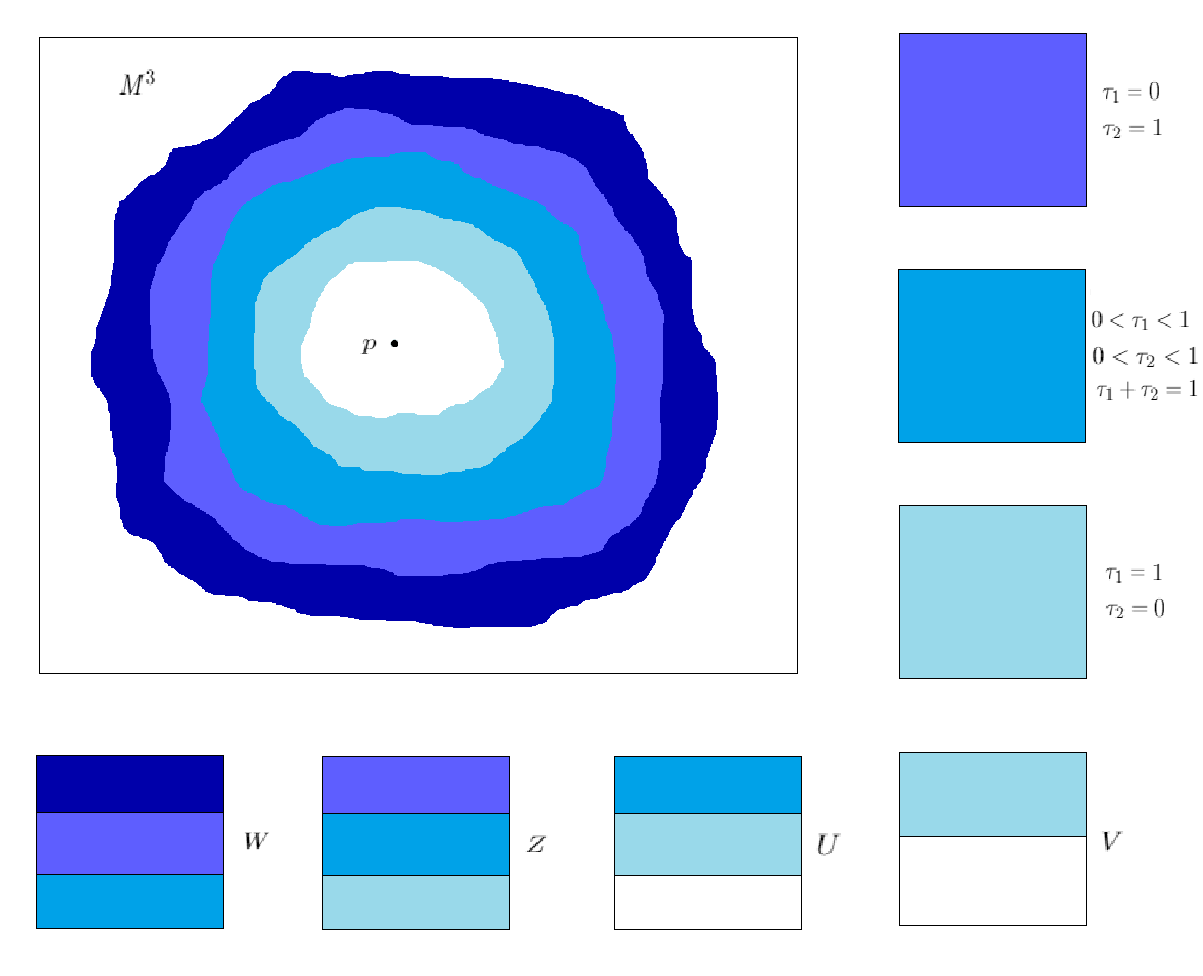
\includegraphics[scale=0.45]{imagenfinal.png}
\caption{Comportamiento de $\tau_{1}$ y $\tau_{2}$, y descripci\'on de los conjuntos $U$, $V$, $W$ y $Z$.}
\label{final}
\end{figure}


\section{Estructuras Simpl\'ecticas Inducidas}\label{3.3}
Terminaremos este trabajo de investigaci\'on describiendo c\'omo son las estructuras simpl\'ecticas en la hojas simpl\'ectias de la foliaci\'on caracter\'istica inducida por los $2-$campos vectoriales locales encontrados en la secci\'on \ref{3.1}.
\vspace{5mm}

Explicaremos brevemente el procedimiento general que utilizaremos para encontrar dichas estructuras simpl\'ecticas.

\begin{description}
    \item[i)] Selecionamos el $2-$campo vectorial $\pi$ como en \ref{pi1}, \ref{pi2}, \ref{pi3}, \ref{pi4} y \ref{pi5}.
    \item[ii)] Seleccionamos los mapeos casimires $C_{1}$ y $C_{2}$ para $\pi$.
    \item[iii)] Obtenemos los vectores tangentes $u_{p}$ y $v_{p}$ a la hoja simpl\'ectica $L_{p}$ en el punto $p\in M$, calculando el espacio nulo de las diferenciales $dC_{1}$ y $dC_{2}$.
    \item[iv)] Utilizamos el $2-$campos vectorial $\pi$ para encontrar $\alpha_{p}$ y $\beta_{p}$ tal que $\pi^{\#}_{p}(\alpha_{p})=u_{p}$ y $\pi^{\#}_{p}(\beta_{p})=v_{p}$.
     \item[v)] Calcular la forma simpl\'ectica utilizando la ecuaci\'on \ref{EcForSimp}. 
\end{description}

\begin{propo}
Sea $p=(x,y,z,t)\in M^{3}\times\mathbb{S}^{1}$ y $\pi$ de la forma \ref{pi1}, \ref{pi2}, \ref{pi3}, \ref{pi4} \'o \ref{pi5}. La forma simpl\'ectica inducida por $\pi$ en la hoja simpl\'ectica $L_{p}$ a trav\'es del punto $p$ de la foliaci\'on simple\'ctica inducida por el $2-$campo vectorial $\pi$ est\'a dada como:  
\begin{equation}\label{eqformasimplectica}
\frac{x}{k(x,y,z,t)\sqrt{x^{2}+y^{2}}}\omega_{area}(p)
\end{equation}
donde $\omega_{area}$ es la forma de \'area en la hoja $L_{p}$ iducida por la m\'etrica euclideana en $M^{3}\times\mathbb{S}^{1}$. 
\end{propo}
\noindent{\bfseries Demostraci\'on.}\\
Asumamos que $x^{2}+y^{2}\neq 0$ y elegimos los mapeos Casimir dependiendo del $2-$campo vectorial $\pi$ elegido.\\

\begin{table}[!ht]
\centering
\begin{tabular}{|c|c|c|l|}
\hline
\multirow{5}{*}{dim$(N_{j})=0$} & Tipo                    & \multicolumn{1}{l|}{\'Indice de Morse} & Mapeos Casimir                                                                                                                                 \\ \cline{2-4} 
                                & \multirow{2}{*}{centro} & cero                             & \begin{tabular}[c]{@{}l@{}}$C_{1}(x,y,z, t)=x^{2}+y^{2}+z^{2}$\\ $C_{2}(x,y,z, t)=t$\end{tabular}    \\ \cline{3-4} 
                                &                         & tres                            & \begin{tabular}[c]{@{}l@{}}$C_{1}(x,y,z, t)=-x^{2}-y^{2}-z^{2}$\\ $C_{2}(x,y,z, t)=t$\end{tabular}   \\ \cline{2-4} 
                                & \multirow{2}{*}{silla} & uno                              & \begin{tabular}[c]{@{}l@{}}$C_{1}(x,y,z, t)=-x^{2}+y^{2}+z^{2}$\\ $C_{2}(x,y,z, t)=t$\end{tabular}   \\ \cline{3-4} 
                                &                         & dos                              & \begin{tabular}[c]{@{}l@{}}$C_{1}(x,y,z, t)=-x^{2}-y^{2}+z^{2}$\\ $C_{2}(x,y,z, t)=t$\end{tabular}   \\ \hline
\multirow{3}{*}{dim$(N_{j})=1$} & \multirow{2}{*}{centro} & cero                             & \begin{tabular}[c]{@{}l@{}}$C_{1}(x,y,z, t)=x^{2}+x^{2}$\\ $C_{2}(x,y,z, t)=t$\end{tabular}              \\ \cline{3-4} 
                                &                         & dos                              & \begin{tabular}[c]{@{}l@{}}$C_{1}(x,y,z, t)=x^{2}+x^{2}$\\ $C_{2}(x,y,z, t)=t$\end{tabular}              \\ \cline{2-4} 
                                & silla                  & uno                              & \begin{tabular}[c]{@{}l@{}}$C_{1}(x,y,z, t)=-x^{2}+y^{2}$\\ $C_{2}(x_{1},x_{2},x_{3}, t)=t$\end{tabular} \\ \hline
\end{tabular}
\caption{Mapeos Casimir consideramos para cada caso de $N_{j}$.}
\label{tabla6}
\end{table}

Con ayuda del programa escrito en c\'odigo de Python explicado a detalle en \ref{A.2}, tenemos los siguientes vectores tangentes $u_{p}$ y $v_{p}$ mostrados en el siguiente cuadro \ref{tabla7}.\\

\begin{table}[!ht]
\centering
%\caption{My caption}
\begin{tabular}{|c|c|c|c|c|}
\hline
\multirow{5}{*}{dim$(N_{j})=0$} & Tipo                    & \multicolumn{1}{l|}{\'Indice de Morse } & $u_{q}$                                                                      & $v_{q}$                                                                                                      \\ \cline{2-5} 
                                & \multirow{2}{*}{centro} & cero                             & $\frac{1}{\sqrt{x^{2}+y^{2}}}(-y\partial_{1}+x\partial_{2})$ & $\frac{-1}{x^{2}+y^{2}}(x^{2}z\partial_{1}+xyz\partial_{2})+x\partial_{3}$ \\ \cline{3-5} 
                                &                         & tres                            & $\frac{1}{\sqrt{x^{2}+y^{2}}}(-y\partial_{1}+x\partial_{2})$ & $\frac{-1}{x^{2}+y^{2}}(x^{2}z\partial_{1}+xyz\partial_{2})+x\partial_{3}$ \\ \cline{2-5} 
                                & \multirow{2}{*}{silla} & uno                              & $\frac{1}{\sqrt{x^{2}+y^{2}}}(y\partial_{1}+x\partial_{2})$  & $\frac{-1}{x^{2}+y^{2}}(x^{2}z\partial_{1}-xyz\partial_{2})+x\partial_{3}$ \\ \cline{3-5} 
                                &                         & dos                              & $\frac{1}{\sqrt{x^{2}+y^{2}}}(-y\partial_{1}+x\partial_{2})$ & $\frac{-1}{x^{2}+y^{2}}(x^{2}z\partial_{1}+xyz\partial_{2})+x\partial_{3}$ \\ \hline
\multirow{3}{*}{dim$(N_{j})=1$} & \multirow{2}{*}{centro} & cero                             & $\frac{1}{\sqrt{x^{2}+y^{2}}}(-y\partial_{1}+x\partial_{2})$ & $x\partial_{3}$                                                                                         \\ \cline{3-5} 
                                &                         & dos                              & $\frac{1}{\sqrt{x^{2}+y^{2}}}(-y\partial_{1}+x\partial_{2})$ & $x\partial_{3}$                                                                                         \\ \cline{2-5} 
                                & silla                  & uno                              & $\frac{1}{\sqrt{x^{2}+y^{2}}}(y\partial_{1}+x\partial_{2})$  & $x\partial_{3}$                                                                                         \\ \hline
\end{tabular}
\caption{Vectores tangentes a las fibras.}
\label{tabla7}
\end{table}

Notemos que estos vectores son anulados por $dC_{1}(q)$ y $dC_{2}(q)$. Adem\'as estos vectores son ortogonales con respecto a la m\'etrica euclideana $dx^{2}+dy^{2}+dz^{2}+dt^{2}$.\\

Ahora para cada caso utilizamos la estructura de Poisson local para encontrar cada $\alpha_{p}$ dependiendo el caso mostrados en el cuadro \ref{tabla8}, con el programa escrito en c\'odigo Python, es f\'acil verificar que $\pi^{\#}_{p}(\alpha_{p})=u_{p}$.

\begin{table}[!ht]
\centering
%\caption{My caption}
\begin{tabular}{|c|c|c|c|}
\hline
\multirow{5}{*}{dim$(N_{j})=0$} & Tipo                    & \multicolumn{1}{l|}{\'Indice de Morse} & $\alpha_{q}$                                                                                                \\ \cline{2-4} 
                                & \multirow{2}{*}{centro} & cero                             & $\frac{-1}{k(x,y,z,t)z\sqrt{x^{2}+y^{2}}}(x\partial_{1}+y\partial_{2})$ \\ \cline{3-4} 
                                &                         & tres                            & $\frac{-1}{k(x,y,z,t)z\sqrt{x^{2}+y^{2}}}(x\partial_{1}+y\partial_{2})$ \\ \cline{2-4} 
                                & \multirow{2}{*}{silla} & uno                              & $\frac{1}{k(x,y,z,t)z\sqrt{x^{2}+y^{2}}}(x\partial_{1}-y\partial_{2})$  \\ \cline{3-4} 
                                &                         & dos                              & $\frac{1}{k(x,y,z,t)z\sqrt{x^{2}+y^{2}}}(x\partial_{1}+y\partial_{2})$  \\ \hline
\multirow{3}{*}{dim$(N_{j})=1$} & \multirow{2}{*}{centro} & cero                             & $\frac{1}{k(x,y,z,t)\sqrt{x^{2}+y^{2}}}(x\partial_{3})$                          \\ \cline{3-4} 
                                &                         & dos                              & $\frac{1}{k(x,y,z,t)\sqrt{x^{2}+y^{2}}}(x\partial_{3})$                          \\ \cline{2-4} 
                                & silla                  & uno                              & $\frac{1}{k(x,y,z,t)\sqrt{x^{2}+y^{2}}}(x\partial_{3})$                          \\ \hline
\end{tabular}
\caption{$\mathcal{B}_{p}(\alpha_{q})=u_{p}$}
\label{tabla8}
\end{table}
    
De la misma manera obtenemos $\beta_{q}$ tal que $\mathcal{B}_{q}(\beta_{q})=v_{q}$.\\

\begin{table}[!ht]
\centering
%\caption{My caption}
\begin{tabular}{|c|c|c|c|}
\hline
\multirow{5}{*}{dim$(N_{j})=0$} & Tipo                    & \multicolumn{1}{l|}{\'Indice de Morse} & $\beta_{q}$                                                                                          \\ \cline{2-4} 
                                & \multirow{2}{*}{centro} & cero                             & $\frac{1}{k(x,y,z,t)x^{2}+y^{2}}(xy\partial_{1}-x^{2}\partial_{2})$  \\ \cline{3-4} 
                                &                         & tres                            & $\frac{1}{k(x,y,z,t)x^{2}+x^{2}}(xy\partial_{1}-x^{2}\partial_{2})$  \\ \cline{2-4} 
                                & \multirow{2}{*}{silla} & uno                              & $\frac{-1}{k(x,y,z,t)x^{2}+y^{2}}(xy\partial_{1}+x^{2}\partial_{2})$ \\ \cline{3-4} 
                                &                         & dos                              & $\frac{1}{k(x,y,z,t)x^{2}+y^{2}}(xy\partial_{1}-x^{2}\partial_{2})$  \\ \hline
\multirow{3}{*}{dim$(N_{j})=1$} & \multirow{2}{*}{centro} & cero                             & $\frac{1}{k(x,y,z,t)y}(x\partial_{1})$                                        \\ \cline{3-4} 
                                &                         & dos                             & $\frac{1}{k(x,y,z,t)y}(x\partial_{1})$                                        \\ \cline{2-4} 
                                & silla                  & uno                              & $\frac{-1}{k(x,y,z,t)y}(x\partial_{1})$                                       \\ \hline
\end{tabular}
\caption{$\mathcal{B}_{q}(\beta_{q})=v_{q}$}
\label{tabla9}
\end{table}

Es f\'acil notar que al calcular la expresi\'on de la forma simpl\'etica para cada caso est\'a dada: 

\begin{eqnarray*}
\omega_{\Gamma_{p}}(u_{p},v_{p}) & = &  \langle \alpha_{p} , v_{p} \rangle \\
                                 & = & -\langle \beta_{p} , u_{p} \rangle \\
                                 & = & \frac{x}{k(x,y,z,t)\sqrt{x^{2}+y^{2}}}\omega_{area}(p)  
\end{eqnarray*}

Para terminar notemos que al restringir el mapeo $k(x,y,z,t)|_{M^{3}}$ obtenemos que $\omega_{\Gamma_{p}}(u_{p},v_{p})$ es una forma simpl\'ectica para la hoja $L_{p}$ de la foliaci\'on simplectica inducida por los $2-$campos vectoriales $\pi$ definidos en $M^{3}$, encontrados en la secci\'on \ref{3.1}. \hfill $\square.$ 

\vspace{5mm}

As\'i concluimos este trabajo de investigaci\'on dejando la siguiente pregunta:
\begin{center}
?`Qu\'e podemos decir de la cohomolog\'ia de Poisson de los $2-$campos vectoriales de Poisson encontrados?
\end{center}
En esta pregunta nos encontramos trabajando para darle pronta respuesta; cabe mencionar que el problema de calcular cohomolog\'ias de Poisson es complicado.  
 
\appendix

\chapter{C\'odigos en Python}\label{A1}

En el siguiente apartado describiremos los c\'odigos que fueron desarrollados durante la elaboraci\'on de esta tesis. El la secci\'on \ref{A.1} se presenta un c\'odigo que fue utilizado para hacer los c\'alculos correspondientes para encontrar las estructuras de Poisson dadas en \ref{3.1}. El c\'odigo que aparece en la secci\'on \ref{A.2} se usa para las estructuras simpl\'ecticas inducidas por las estructuras de Poisson dadas en \ref{3.2}. En la secci\'on \ref{A.3} se presenta un c\'odigo que fue desarrollado para comprobar cuando un bivector es de Poisson, es decir, calculamos $[\pi,\pi]$.\\ 

Todos los c\'odigos presentados  aqu\'i fueron elaborados en el lenguaje de programaci\'on Python, utilizando las m\'odulos Sympy \cite{sympy} y Galgebra \cite{galgebra}.  
       
\section{Estructuras de Poisson}\label{A.1}

A continuaci\'on explicaremos como funciona el c\'odigo que calcula la estructura de Poisson mediante peque\~{n}os {\it scripts}. El c\'odigo esta basado de la f\'ormula \ref{EcuRatiu} de Flaska-Ratiu, recordemos que dicho c\'odigo necesita de dos funciones Casimir para poder calcular la estructura de Poisson.

\vspace{5mm}

Empezamos importando el m\'odulo sympy\footnote{Para m\'as imformaci\'on sobre sympy consultar \url{http://docs.sympy.org/latest/index.html}}, el cual se utiliza para desarrollar c\'alculo simb\'olico en python.   

\begin{lstlisting}[frame=single]
import sympy as sym
\end{lstlisting}
Definimos las variables simb\'olicas $x$, $y$, $z$ y $t$ con las cuales describimos los modelos locales de las singularidades de la foliaci\'on $M\times \mathbb{S}^{1}$, as\'i como las variables simb\'olicas $a12$, $a13$, $a14$, $a23$, $a24$ y $a34$ que ser\'an las entradas de la matriz $P$, que definiremos m\'as adelante.     
\begin{lstlisting}[frame=single]
x = sym.Symbol('x')
y = sym.Symbol('y')
z = sym.Symbol('z')
t = sym.Symbol('t')
k = sym.Symbol('k')

a12 = sym.Symbol('a12')
a13 = sym.Symbol('a13')
a14 = sym.Symbol('a14')
a23 = sym.Symbol('a23')
a24 = sym.Symbol('a24')
a34 = sym.Symbol('a34')
\end{lstlisting}
Escribimos los modelos locales de las singularidades de foliaci\'on $M\times\mathbb{S}^1$ que son:
\[ F(x,y,z,t) = \left\{ \begin{array}{lcccc}
             ( x^2+y^2+z^2,t) & si & dim(N_{j})=0 & y & im=0 \\
             (-x^2+y^2+z^2,t) & si & dim(N_{j})=0 & y & im=1 \\
             (-x^2-y^2+z^2,t) & si & dim(N_{j})=0 & y & im=2 \\
             (-x^2-y^2-z^2,t) & si & dim(N_{j})=0 & y & im=3 \\
             ( x^2+y^2,t) & si & dim(N_{j})=1 & y & im=0 \\
             (-x^2+y^2,t) & si & dim(N_{j})=1 & y & im=1 \\
             (-x^2-y^2,t) & si & dim(N_{j})=1 & y & im=2 
             \end{array}
   \right. \]
donde $im$ denotar\'a el \'indice de Morse de $f(x,y,z)$. As\'i tenemos que \texttt{faux}$=t$ y \texttt{f0}$=x^2+y^2+z^2$ en esta caso, ya que es la \'unica que no esta comentada en el c\'odigo.
\begin{lstlisting}
faux = t
f0 = x**2+y**2+z**2
# Esto es un comentario en python
# f0 = -x**2+y**2+z**2 
# f0 = -x**2-y**2+z**2
# f0 = -x**2-y**2-z**2
# f0 = x**2+y**2
# f0 = -x**2+y**2
# f0 = -x**2-y**2
\end{lstlisting}
Definimos la matriz antisim\'etrica 
\[  M = \left( \begin{array}{cccc}
              0   & a12  & a13  & a14  \\
             -a12 & 0    & a23  & a24  \\
             -a13 & -a23 & 0    & a34  \\
             -a14 & -a24 & -a34 & 0   
             \end{array}
   \right). \]
\begin{lstlisting}
P = sym.Matrix ([[0, a12, a13, a14,], [-a12, 0, a23, a24], [-a13, -a23, 0, a34], [-a14, -a24, -a34, 0]])
\end{lstlisting}
Definimos una funci\'on que llamaremos \texttt{EstPoisson} e inmediatamente calculamos el gradiente de la funci\'on \texttt{f0}. 
\begin{lstlisting}    
    def EstPoisson():
        Gra = sym.Matrix ([[sym.diff(faux,x), sym.diff(f0,x)],[sym.diff(faux,y), sym.diff(f0,y)],[sym.diff(faux,z), sym.diff(f0,z)],[sym.diff(faux,t),sym.diff(f0,t)]])
\end{lstlisting}
De lo anterior obtenemos 
\[ Gra = \left( \begin{array}{cccc}
               \frac{\partial f0}{\partial x} & \frac{\partial f0}{\partial y} & \frac{\partial f0}{\partial z} & \frac{\partial f0}{\partial t}  \\
               \frac{\partial faux}{\partial x} & \frac{\partial faux}{\partial y} &  \frac{\partial faux}{\partial z} & \frac{\partial faux}{\partial t}    
             \end{array}
   \right).\] 
Ahora calculamos  
\[ S1 = \left( \begin{array}{cccc}
              0   & a12  & a13  & a14  \\
             -a12 & 0    & a23  & a24  \\
             -a13 & -a23 & 0    & a34  \\
             -a14 & -a24 & -a34 & 0   
             \end{array}
   \right) \cdot \left( \begin{array}{c}
               			\frac{\partial f0}{\partial x} \\
               			\frac{\partial f0}{\partial y} \\ 
               			\frac{\partial f0}{\partial z} \\
               			\frac{\partial f0}{\partial t}  
                   		\end{array}
                 \right).\]   
\begin{lstlisting}
        A = (M*Gra[:,0]).row(0)[0]
        B = (M*Gra[:,0]).row(1)[0]
        C = (M*Gra[:,0]).row(2)[0]
        D = (M*Gra[:,0]).row(3)[0]
\end{lstlisting}
y\\
\[ S2 = \left( \begin{array}{cccc}
              0   & a12  & a13  & a14  \\
             -a12 & 0    & a23  & a24  \\
             -a13 & -a23 & 0    & a34  \\
             -a14 & -a24 & -a34 & 0   
             \end{array}
   \right) \cdot \left( \begin{array}{c}
               			\frac{\partial faux}{\partial x} \\
               			\frac{\partial faux}{\partial y} \\ 
               			\frac{\partial faux}{\partial z} \\
               			\frac{\partial faux}{\partial t} 
                   		\end{array}
                 \right).\] 
\begin{lstlisting}  
        E = (P*Gra[:,1]).row(0)[0]        
        F = (P*Gra[:,1]).row(1)[0]
        G = (P*Gra[:,1]).row(2)[0]
        H = (P*Gra[:,1]).row(3)[0]
\end{lstlisting}    

Resolvemos simult\'aneamente los sistemas $S1=0$ y $S2=0$, y guardamos los valores obtenidos en las variables simb\'olicas \texttt{A12}, \texttt{A13}, \texttt{A14}, \texttt{A23}, \texttt{A24} y \texttt{A34}.     
\begin{lstlisting} 
        A12,A13,A14,A23,A24,A34 = list(sym.linsolve([A,B,C,D,E,F,G,H],(a12,a13,a14,a23,a24,a34)))[0]
\end{lstlisting}
Para finalizar la funci\'on \texttt{EstPoisson}, asignamos los valores $A12$, $A13$, $A14$, $A23$, $A24$ y $A34$ a una nueva matriz $N$, que es la matriz de Poisson buscada.     
\begin{lstlisting}
        N = sym.Matrix ([[0, A12, A13, A14,], [-A12, 0, A23, A24], [-A13, -A23, 0,A34], [-A14, -A24, -A34, 0]])
    return N
\end{lstlisting}
Al unir todos los bloques de scripts anteriores, nuestro c\'odigo de Python se ver\'a de la siguiente manera.   
\lstset{stepnumber=1}
\begin{lstlisting}
import sympy as sym

x = sym.Symbol('x')
y = sym.Symbol('y')
z = sym.Symbol('z')
t = sym.Symbol('t')
k = sym.Symbol('k')

a12 = sym.Symbol('a12')
a13 = sym.Symbol('a13')
a14 = sym.Symbol('a14')
a23 = sym.Symbol('a23')
a24 = sym.Symbol('a24')
a34 = sym.Symbol('a34')

faux = t
f0 = x**2+y**2+z**2
# f0 = -x**2+y**2+z**2 
# f0 = -x**2-y**2+z**2
# f0 = -x**2-y**2-z**2
# f0 = x**2+y**2
# f0 = -x**2+y**2
# f0 = -x**2-y**2

P = sym.Matrix ([[0, a12, a13, a14,], [-a12, 0, a23, a24], [-a13, -a23, 0, a34], [-a14, -a24, -a34, 0]])

def EstPoisson():
    Gra = sym.Matrix ([[sym.diff(faux,x), sym.diff(f0,x)],[sym.diff(faux,y), sym.diff(f0,y)],[sym.diff(faux,z), sym.diff(f0,z)],[sym.diff(faux,t),sym.diff(f0,t)]])
    A = (P*Gra[:,0]).row(0)[0]
    B = (P*Gra[:,0]).row(1)[0]
    C = (P*Gra[:,0]).row(2)[0]
    D = (P*Gra[:,0]).row(3)[0]
    E = (P*Gra[:,1]).row(0)[0]
    F = (P*Gra[:,1]).row(1)[0]
    G = (P*Gra[:,1]).row(2)[0]
    H = (P*Gra[:,1]).row(3)[0]
    A12,A13,A14,A23,A24,A34 = list(sym.linsolve([A,B,C,D,E,F,G,H],(a12,a13,a14,a23,a24,a34)))[0]
    N = sym.Matrix ([[0, A12, A13, A14,], [-A12, 0, A23, A24], [-A13, -A23, 0,A34], [-A14, -A24, -A34, 0]])
    return N

print(EstPoisson())
\end{lstlisting}
Para poder ejecutar el c\'odigo copie y pegue el script anterior, configure el archivo en las variables correspondientes, guarde el archivo con el nombre \texttt{poisson.py} por ejemplo y por \'ultimo abr\'a la consola (ventana de comandos) en el directorio donde se encuentra el archivo \texttt{poisson.py} y escriba \texttt{python poisson.py}.  

\section{La Estructura Simpl\'ectica Inducida}\label{A.2}
Para explicar el c\'odigo que hace el c\'alculo de la estructura simpl\'ectica inducida por una estructura de Poisson, debemos tener presente que necesitamos del c\'odigo presentado en la secci\'on \ref{A.1}. En esta secci\'on s\'olo nos limitamos a explicar la funci\'on \texttt{EstSimplectica}.\\

Definimos la funci\'on, obtenemos el gradiente del mapeo f0 y calculamos una base para su espacio nulo.  
\lstset{stepnumber=0}
\begin{lstlisting}
    def EstSimplectica():
        Gra = sym.Matrix ([[sym.diff(f0,x), sym.diff(faux,x)],[sym.diff(f0,y), sym.diff(faux,y)],[sym.diff(f0,z), sym.diff(faux,z)],[sym.diff(f0,t),sym.diff(faux,t)]])
        Ker1 = (Gra.T).nullspace()[0]
        Ker2 = (Gra.T).nullspace()[1]
\end{lstlisting}
Dada la base del espacio nulo del gradiente de f0, obtenemos un base ortonogonal mediante el proceso de Gram-Schmidt, para as\'i obtener los vectores $U_{q}$ y $V_{q}$. Est\'a base ortogonal ayudar\'a a facilitar los c\'alculos.   
\lstset{stepnumber=0}
\begin{lstlisting}
        GS = sym.GramSchmidt([Ker1,Ker2], orthonormal=False)
        Uq = GS[0]/(sym.sqrt(GS[0].dot(GS[0])))
        Vq = sym.simplify(GS[1])  
\end{lstlisting}
Llamamos la funci\'on \texttt{EstPoisson} definida en \ref{A.1}.
\lstset{stepnumber=0}
\begin{lstlisting}
N = EstPoisson()
\end{lstlisting}
Definimos las variables simb\'olicas $a$,$b$,$c$ y $d$, para obtener el vector columna 
\[ \left( \begin{array}{c}
             a  \\
             b  \\
             c  \\
             d     
             \end{array}
   \right). \] 
\lstset{stepnumber=0}
\begin{lstlisting}
        a = sym.Symbol('a')
        b = sym.Symbol('b')
        c = sym.Symbol('c')
        d = sym.Symbol('d') 
        alfa = sym.Matrix([[a],[b],[c],[d]])
\end{lstlisting}
Ahora calculamos 
\[ S1 = \left( \begin{array}{cccc}
              0   & A12  & A13  & A14  \\
             -A12 & 0    & A23  & A24  \\
             -A13 & -A23 & 0    & A34  \\
             -A14 & -A24 & -A34 & 0   
             \end{array}
   \right) \cdot \left( \begin{array}{c}
               			a \\
               			b \\ 
               			c \\
               			d \\
                   		\end{array}
                 \right)- \left( \begin{array}{c}
               			U_{q_{1}} \\
               			U_{q_{2}} \\ 
               			U_{q_{3}}\\
               			U_{q_{4}} \\
                   		\end{array}
                 \right) ,\]
mediante el siguiente script.
\lstset{stepnumber=0}
\begin{lstlisting} 
        X = (N*alfa)-Uq
        X1 = ((N*alfa)-Uq).row(0)[0]
        X2 = ((N*alfa)-Uq).row(1)[0]
        X3 = ((N*alfa)-Uq).row(2)[0]
        X4 = ((N*alfa)-Uq).row(3)[0]
\end{lstlisting}
Resolvemos el sistema $S1=0$ y asignamos los valores encontrados a las variables $A$, $B$, $C$ y $D$ para formar el vector
\[ \alpha = \left( \begin{array}{c}
               			A \\
               			B \\ 
               			C \\
               			D \\
                   		\end{array}
                 \right) .\] 
\lstset{stepnumber=0}
\begin{lstlisting}
A,B,C,D = list(sym.linsolve([X1,X2,X3,X4],(a,b,c,d)))[0]
        alpha = sym.Matrix([[A],[B],[C],[D]])
\end{lstlisting}
Definimos las variables simb\'olicas $e$, $g$, $h$ y $j$, para obtener el vector columna 
\[ \left( \begin{array}{c}
             e  \\
             g  \\
             h  \\
             j     
             \end{array}
   \right). \] 
\lstset{stepnumber=0}
\begin{lstlisting}
        e = sym.Symbol('e')
        g = sym.Symbol('g')
        h = sym.Symbol('h')
        j = sym.Symbol('j')            
        betha = sym.Matrix([[e],[g],[h],[j]])
\end{lstlisting}
Ahora calculamos 
\[ S2 = \left( \begin{array}{cccc}
              0   & A12  & A13  & A14  \\
             -A12 & 0    & A23  & A24  \\
             -A13 & -A23 & 0    & A34  \\
             -A14 & -A24 & -A34 & 0   
             \end{array}
   \right) \cdot \left( \begin{array}{c}
               			e \\
               			g \\ 
               			h \\
               			j \\
                   		\end{array}
                 \right)- \left( \begin{array}{c}
               			V_{q_{1}} \\
               			V_{q_{2}} \\ 
               			V_{q_{3}}\\
               			V_{q_{4}} \\
                   		\end{array}
                 \right) .\]
\lstset{stepnumber=0}
\begin{lstlisting}
        Y = (N*betha)-Vq
        Y1 = ((N*betha)-Vq).row(0)[0]
        Y2 = ((N*betha)-Vq).row(1)[0]
        Y3 = ((N*betha)-Vq).row(2)[0]
        Y4 = ((N*betha)-Vq).row(3)[0]
\end{lstlisting}
Resolvemos el sistema $S2=0$ y asignamos los valores encontrados a las variables $A$, $B$, $C$ y $D$ para formar el vector
\[ \beta = \left( \begin{array}{c}
               			E \\
               			G \\ 
               			H \\
               			J \\
                   		\end{array}
                 \right) \] 

\lstset{stepnumber=0}
\begin{lstlisting}
        E,G,H,J = list(sym.linsolve([Y1,Y2,Y3,Y4],(e,g,h,j)))[0]
        beta = sym.Matrix([[E],[G],[H],[J]])
\end{lstlisting}
Calculamos la formas simpl\'ecticas como sigue, $w_{1}=\langle\alpha,V_{q}\rangle$ y $w_{2}=\langle\beta,U_{q}\rangle$.   
\lstset{stepnumber=0}
\begin{lstlisting}
        w1 =  sym.simplify(alpha.dot(Vq))
        w2 =  sym.simplify(-beta.dot(Uq))
        Comp = sym.simplify(w1-w2)
\end{lstlisting}
Por \'ultimo la funci\'on EstSimplectica no debe regresar la forma simpl\'ectica $w_{1}$, $w_{2}$ y la comprobaci\'on que las mismas son iguales. 
\lstset{stepnumber=0}
\begin{lstlisting}
    return  [w1, w2, Comp]
\end{lstlisting}
Juntando todos los scripts anteriores, el programa para calcular la estructura simpl\'ectica inducida por una estructura de Poisson se ve de la siguiente forma.  
\lstset{stepnumber=1}
\begin{lstlisting}
def EstSimplectica():
    Gra = sym.Matrix ([[sym.diff(f0,x), sym.diff(faux,x)],[sym.diff(f0,y), sym.diff(faux,y)],[sym.diff(f0,z), sym.diff(faux,z)],[sym.diff(f0,t),sym.diff(faux,t)]])
    Ker1 = (Gra.T).nullspace()[0]
    Ker2 = (Gra.T).nullspace()[1]
    
    GS = sym.GramSchmidt([Ker1,Ker2], orthonormal=False)
    Uq = GS[0]/(sym.sqrt(GS[0].dot(GS[0])))
    Vq = sym.simplify(GS[1])
     
    N = EstPoisson()
    a = sym.Symbol('a')
    b = sym.Symbol('b')
    c = sym.Symbol('c')
    d = sym.Symbol('d') 
    alfa = sym.Matrix([[a],[b],[c],[d]])
    X = (N*alfa)-Uq
    X1 = ((N*alfa)-Uq).row(0)[0]
    X2 = ((N*alfa)-Uq).row(1)[0]
    X3 = ((N*alfa)-Uq).row(2)[0]
    X4 = ((N*alfa)-Uq).row(3)[0]
    A,B,C,D = list(sym.linsolve([X1,X2,X3,X4],(a,b,c,d)))[0]
    alpha = sym.Matrix([[A],[B],[C],[D]])
    
    e = sym.Symbol('e')
    g = sym.Symbol('g')
    h = sym.Symbol('h')
    j = sym.Symbol('j')            
    betha = sym.Matrix([[e],[g],[h],[j]])
    Y = (N*betha)-Vq
    Y1 = ((N*betha)-Vq).row(0)[0]
    Y2 = ((N*betha)-Vq).row(1)[0]
    Y3 = ((N*betha)-Vq).row(2)[0]
    Y4 = ((N*betha)-Vq).row(3)[0]
    E,G,H,J = list(sym.linsolve([Y1,Y2,Y3,Y4],(e,g,h,j)))[0]
    beta = sym.Matrix([[E],[G],[H],[J]])
    
    w1 =  sym.simplify(alpha.dot(Vq))
    w2 =  sym.simplify(-beta.dot(Uq))
    Comp = sym.simplify(w1-w2)  
	return [w1, w2, Comp] 
\end{lstlisting}
Para poder ejecutar el c\'odigo copie y pegue la funci\'on \texttt{EstPoisson} de la secci\'on \ref{A.1} antes de la funci\'on \texttt{EstSimplectica} configure el archivo en las variables correspondientes, guarde el archivo con el nombre \texttt{poisson.py} por ejemplo y por \'ultimo abr\'a la consola (ventana de comandos) en el directorio donde se encuentra el archivo \texttt{poisson.py} y escriba \texttt{python poisson.py}.  

\section{El Corchete de Schouten-Nijenhuis}\label{A.3}
Explicaremos a detalle mediante scripts como funciona el c\'odigo para calcular el corchete de Schouten-Nijenhuis (definido como en la secci\'on \ref{2.2}) de un $2-$campo vectorial consigo mismo y poder determinar cuand un bivector es de Poisson. Empezamos importando los m\'odulos sympy y ga\footnote{Para m\'as imformaci\'on sobre \texttt{ga} recomendamos consultar \url{https://github.com/brombo/galgebra}}(galgebra), el cual ocupamos para poder operar el producto exterior.
\lstset{stepnumber=0}
\begin{lstlisting}
import ga
import sympy as sym
\end{lstlisting}

Definimos la variables que vamos a utilizar, donde $dij:=\frac{\partial }{\partial x_{1}}\wedge\frac{\partial }{\partial x_{j}}$, con $i\in\{1,2,3,4\}$ y $j\in\{2,3,4\}$
\lstset{stepnumber=0}
\begin{lstlisting}
x1 = sym.Symbol('x1')
x2 = sym.Symbol('x2')
x3 = sym.Symbol('x3')
x4 = sym.Symbol('x4')

d12 = sym.Symbol('d12')
d13 = sym.Symbol('d13')
d14 = sym.Symbol('d14')
d23 = sym.Symbol('d23')
d24 = sym.Symbol('d24')
d34 = sym.Symbol('d34')
\end{lstlisting}
Definimos una m\'etrica en $\mathbb{R}^{4}$, utilizando un met\'odo de \texttt{ga}.
\lstset{stepnumber=0}
\begin{lstlisting}
g4coords = (x1,x2,x3,x4)
g4 = ga.Ga('dx1 dx2 dx3 dx4', g=[1,1,1,1], coords=g4coords) 
(dx1, dx2 , dx3, dx4) = g4.mv()
\end{lstlisting}
Recordemos que un bivector se puede escribir como 
\begin{eqnarray*}
\pi & = & f_{1}\frac{\partial}{\partial x_{1}}\wedge\frac{\partial}{\partial x_{2}}+f_{2}\frac{\partial}{\partial x_{1}}\wedge\frac{\partial}{\partial x_{3}}+f_{3}\frac{\partial}{\partial x_{1}}\wedge\frac{\partial}{\partial x_{4}} \\
    & + & f_{4}\frac{\partial}{\partial x_{2}}\wedge\frac{\partial}{\partial x_{3}}+f_{5}\frac{\partial}{\partial x_{2}}\wedge\frac{\partial}{\partial x_{4}}+f_{6}\frac{\partial}{\partial x_{3}}\wedge\frac{\partial}{\partial x_{4}},
\end{eqnarray*}
donde $f_{i}\in C^{\infty}(\mathbb{R}^{4})$.
\lstset{stepnumber=0}
\begin{lstlisting}
f1 = 0
f2 = -x2
f3 = 0
f4 = x1
f5 = 0
f6 = 0

Pi = f1*(dx1^dx2) + f2*(dx1^dx3) + f3*(dx1^dx4) + f4*(dx2^dx3) + f5*(dx2^dx4) + f6*(dx3^dx4) 
Piaux = f1*d12 + f2*d13 + f3*d14 + f4*d23 + f5*d24 + f6*d34
\end{lstlisting}
Definimos la funci\'on SN 
\lstset{stepnumber=0}
\begin{lstlisting}
def SN():
\end{lstlisting}
Ahora vamos a calcular $\frac{\partial\Pi}{\partial\xi_{1}}$ con el siguiente script.
\lstset{stepnumber=0}
\begin{lstlisting}
    dEspPix1a = (sym.diff(Piaux,d12))*(dx2) #dPi/d(dx1) para la forma dx1^dx2
    dEspPix1b = (sym.diff(Piaux,d13))*(dx3) #dPi/d(dx1) para la forma dx1^dx3
    dEspPix1c = (sym.diff(Piaux,d14))*(dt)  #dPi/d(dx1) para la forma dx1^dx4 
\end{lstlisting}
An\'alogamente, calculamos el resto de las derivadas parciales con los scripts que se muestran a continuaci\'on.
\begin{itemize}
    \item $$\frac{\partial \pi}{\partial x_{1}}.$$
\lstset{stepnumber=0}
\begin{lstlisting}
    dNorPix1a = (sym.diff(f1,x1))*(dx1^dx2) #(df1/dx1)^(dx1^dx2)  
    dNorPix1b = (sym.diff(f2,x1))*(dx1^dx3) #(df2/dx1)^(dx1^dx3)
    dNorPix1c = (sym.diff(f3,x1))*(dx1^dx4) #(df3/dx1)^(dx1^dx4)
    dNorPix1d = (sym.diff(f4,x1))*(dx2^dx3) #(df4/dx1)^(dx2^dx3)
    dNorPix1e = (sym.diff(f5,x1))*(dx2^dx4) #(df5/dx1)^(dx2^dx4)
    dNorPix1f = (sym.diff(f6,x1))*(dx3^dx4) #(df6/dx1)^(dx3^dx4)
\end{lstlisting}
\item $$\frac{\partial \pi}{\partial \xi_{2}}.$$
\lstset{stepnumber=0}
\begin{lstlisting}
    dEspPix2a = -(sym.diff(Piaux,d12))*(dx1) #dPi/d(dx2) para la forma dx1^dx2 
    dEspPix2b = (sym.diff(Piaux,d23))*(dx3) #dPi/d(dx2) para la forma dx2^dx3
    dEspPix2c = (sym.diff(Piaux,d24))*(dx4) #dPi/d(dx2) para la forma dx3^dx4
\end{lstlisting}
\item $$\frac{\partial \pi}{\partial x_{2}}.$$
\lstset{stepnumber=0}
\begin{lstlisting}
    dNorPix2a = (sym.diff(f1,x2))*(dx1^dx2) #(df1/dx2)^(dx1^dx2)
    dNorPix2b = (sym.diff(f2,x2))*(dx1^dx3) #(df2/dx2)^(dx1^dx3)
    dNorPix2c = (sym.diff(f3,x2))*(dx1^dx4) #(df3/dx2)^(dx1^dx4)
    dNorPix2d = (sym.diff(f4,x2))*(dx2^dx3) #(df4/dx2)^(dx2^dx3)
    dNorPix2e = (sym.diff(f5,x2))*(dx2^dx4) #(df5/dx2)^(dx2^dx4)
    dNorPix2f = (sym.diff(f6,x2))*(dx3^dx4) #(df6/dx2)^(dx3^dx4)
\end{lstlisting}
\item $$\frac{\partial \pi}{\partial \xi_{3}}.$$
\lstset{stepnumber=0}
\begin{lstlisting}
    dEspPix3a = -(sym.diff(Piaux,d13))*(dx1) #dPi/dx3 para la forma dx1^dx3
    dEspPix3b = -(sym.diff(Piaux,d23))*(dx2) #dPi/dx3 para la forma dx2^dx3
    dEspPix3c = (sym.diff(Piaux,d34))*(dx4) #dPi/dx3 para la forma dx3^dx4
\end{lstlisting}
\item $$\frac{\partial \pi}{\partial x_{3}}.$$
\lstset{stepnumber=0}
\begin{lstlisting}
    dNorPix3a = (sym.diff(f1,x3))*(dx1^dx2) #(df1/dx3)^(dx1^dx2)
    dNorPix3b = (sym.diff(f2,x3))*(dx1^dx3) #(df2/dx3)^(dx1^dx3)
    dNorPix3c = (sym.diff(f3,x3))*(dx1^dx4) #(df3/dx3)^(dx1^dx4)
    dNorPix3d = (sym.diff(f4,x3))*(dx2^dx3) #(df4/dx3)^(dx2^dx3)
    dNorPix3e = (sym.diff(f5,x3))*(dx2^dx4) #(df5/dx3)^(dx2^dx4)
    dNorPix3f = (sym.diff(f6,x3))*(dx3^dx4) #(df6/dx3)^(dx3^dx4)
\end{lstlisting}
\item $$\frac{\partial \pi}{\partial \xi_{4}}.$$
\lstset{stepnumber=0}
\begin{lstlisting}
    dEspPix4a = -(sym.diff(Piaux,d14))*(dx1)  #dPi/d(dx4) para la forma dx1^dx4
    dEspPix4b = -(sym.diff(Piaux,d24))*(dx2)  #dPi/d(dx4) para la forma dx2^dx4
    dEspPix4c = -(sym.diff(Piaux,d34))*(dx3)  #dPi/d(dx4) para la forma dx3^dx4
\end{lstlisting}
\item $$\frac{\partial \pi}{\partial x_{4}}.$$
\lstset{stepnumber=0}
\begin{lstlisting}
    dNorPix4a = (sym.diff(f1,x4))*(dx1^dx2) #(df1/dx4)^(dx1^dx2)
    dNorPix4b = (sym.diff(f2,x4))*(dx1^dx3) #(df2/dx4)^(dx1^dx3)
    dNorPix4c = (sym.diff(f3,x4))*(dx1^dx4) #(df3/dx4)^(dx1^dx4)
    dNorPix4d = (sym.diff(f4,x4))*(dx2^dx3) #(df4/dx4)^(dx2^dx3)
    dNorPix4e = (sym.diff(f5,x4))*(dx2^dx4) #(df5/dx4)^(dx2^dx4)
    dNorPix4f = (sym.diff(f6,x4))*(dx3^dx4) #(df6/dx4)^(dx3^dx4)
\end{lstlisting}
\end{itemize}
Con todos los scripts anteriores podemos calcular el corchete Schouten-Nijenhuis, que para este caso queda de la siguiente manera:
\begin{equation*}
[\pi,\pi]  =  \Sigma_{i=i}^{4}2\left( \frac{\partial \pi}{\partial \xi_{i}}\wedge\frac{\partial \pi}{\partial x_{i}} \right), 
\end{equation*} 
donde $\xi_{i}=\frac{\partial }{\partial x_{i}}$. Obteniendo como resultado de la funci\'on $[\pi,\pi]$, definida por: 
\lstset{stepnumber=0}
\begin{lstlisting}
    SNPi = 2*((dEspPix1a+dEspPix1b+dEspPix1c)^(dNorPix1a+dNorPix1b+dNorPix1c+dNorPix1d+dNorPix1e+dNorPix1f)) + 2*((dEspPix2a+dEspPix2b+dEspPix2c)^(dNorPix2a+dNorPix2b+dNorPix2c+dNorPix2d+dNorPix2e+dNorPix2f)) + 2*((dEspPix3a+dEspPix3b+dEspPix3c)^(dNorPix3a+dNorPix3b+dNorPix3c+dNorPix3d+dNorPix3e+dNorPix3f)) + 2*((dEspPita+dEspPitb+dEspPitc)^(dNorPita+dNorPitb+dNorPitc+dNorPitd+dNorPite+dNorPitf))
    return SNPi    
\end{lstlisting}
Uniendo todos los scripts anteriores tenemos que el programa para calcular el corchete de Schouten-Nijenhuis queda as\'i.
\lstset{stepnumber=1}
\begin{lstlisting}
import ga
import sympy as sym

x1 = sym.Symbol('x1')
x2 = sym.Symbol('x2')
x3 = sym.Symbol('x3')
x4 = sym.Symbol('x4')

d12 = sym.Symbol('d12')
d13 = sym.Symbol('d13')
d14 = sym.Symbol('d14')
d23 = sym.Symbol('d23')
d24 = sym.Symbol('d24')
d34 = sym.Symbol('d34')

g4coords = (x1,x2,x3,x4)
g4 = ga.Ga('dx1 dx2 dx3 dx4', g=[1,1,1,1], coords=g4coords) 
(dx1, dx2 , dx3, dx4) = g4.mv()

f1 = 0
f2 =-x2
f3 = 0
f4 = x1
f5 = 0
f6 = 0

Pi = f1*(dx1^dx2)+f2*(dx1^dx3)+f3*(dx1^dx4)+f4*(dx2^dx3)+f5*(dx2^dx4)+f6*(dx3^dx4) 

Piaux = f1*d12+f2*d13+f3*d14+f4*d23+f5*d24+f6*d34

def SN():
    # Derivada especial de Pi para dx1 
    dEspPix1a = (sym.diff(Piaux,d12))*(dx2) # dPi/d(dx1) para la forma dx1^dx2
    dEspPix1b = (sym.diff(Piaux,d13))*(dx3) # dPi/d(dx1) para la forma dx1^dx3
    dEspPix1c = (sym.diff(Piaux,d14))*(dx4) # dPi/d(dx1) para la forma dx1^dx4 
    # Derivada normal de Pi para x1
    dNorPix1a = (sym.diff(f1,x1))*(dx1^dx2) # (df1/dx1)^(dx1^dx2)  
    dNorPix1b = (sym.diff(f2,x1))*(dx1^dx3) # (df2/dx1)^(dx1^dx3)
    dNorPix1c = (sym.diff(f3,x1))*(dx1^dx4) # (df3/dx1)^(dx1^dx4)
    dNorPix1d = (sym.diff(f4,x1))*(dx2^dx3) # (df4/dx1)^(dx2^dx3)
    dNorPix1e = (sym.diff(f5,x1))*(dx2^dx4) # (df5/dx1)^(dx2^dx4)
    dNorPix1f = (sym.diff(f6,x1))*(dx3^dx4) # (df6/dx1)^(dx3^dx4)

    # Derivada especial de Pi para dx2
    dEspPix2a = -(sym.diff(Piaux,d12))*(dx1) # dPi/d(dx2) para la forma dx1^dx2 
    dEspPix2b = (sym.diff(Piaux,d23))*(dx3)  # dPi/d(dx2) para la forma dx2^dx3
    dEspPix2c = (sym.diff(Piaux,d24))*(dx4)  # dPi/d(dx2) para la forma dx3^dx4
    # Derivada normal de Pi para x2 
    dNorPix2a = (sym.diff(f1,x2))*(dx1^dx2) # (df1/dx2)^(dx1^dx2)
    dNorPix2b = (sym.diff(f2,x2))*(dx1^dx3) # (df2/dx2)^(dx1^dx3)
    dNorPix2c = (sym.diff(f3,x2))*(dx1^dx4) # (df3/dx2)^(dx1^dx4)
    dNorPix2d = (sym.diff(f4,x2))*(dx2^dx3) # (df4/dx2)^(dx2^dx3)
    dNorPix2e = (sym.diff(f5,x2))*(dx2^dx4) # (df5/dx2)^(dx2^dx4)
    dNorPix2f = (sym.diff(f6,x2))*(dx3^dx4) #(df6/dx2)^(dx3^dx4)
    
    # Derivada especial de Pi para dx3
    dEspPix3a = -(sym.diff(Piaux,d13))*(dx1) # dPi/dx3 para la forma dx1^dx3
    dEspPix3b = -(sym.diff(Piaux,d23))*(dx2) # dPi/dx3 para la forma dx2^dx3
    dEspPix3c = (sym.diff(Piaux,d34))*(dx4)  # dPi/dx3 para la forma dx3^dx4
    # Derivada normal de Pi para x3 
    dNorPix3a = (sym.diff(f1,x3))*(dx1^dx2) # (df1/dx3)^(dx1^dx2)
    dNorPix3b = (sym.diff(f2,x3))*(dx1^dx3) # (df2/dx3)^(dx1^dx3)
    dNorPix3c = (sym.diff(f3,x3))*(dx1^dx4) # (df3/dx3)^(dx1^dx4)
    dNorPix3d = (sym.diff(f4,x3))*(dx2^dx3) # (df4/dx3)^(dx2^dx3)
    dNorPix3e = (sym.diff(f5,x3))*(dx2^dx4) # (df5/dx3)^(dx2^dx4)
    dNorPix3f = (sym.diff(f6,x3))*(dx3^dx4) # (df6/dx3)^(dx3^dx4)
    
    # Derivada especial de Pi para dt 
    dEspPix4a = -(sym.diff(Piaux,d14))*(dx1)  # dPi/d(dx4) para la forma dx1^dx4
    dEspPix4b = -(sym.diff(Piaux,d24))*(dx2)  # dPi/d(dx4) para la forma dx2^dx4
    dEspPix4c = -(sym.diff(Piaux,d34))*(dx3)  # dPi/d(dx4) para la forma dx3^dx4
    # Derivada normal de Pi para t 
    dNorPix4a = (sym.diff(f1,x4))*(dx1^dx2)  # (df1/dx4)^(dx1^dx2)
    dNorPix4b = (sym.diff(f2,x4))*(dx1^dx3)  # (df2/dx4)^(dx1^dx3)
    dNorPix4c = (sym.diff(f3,x4))*(dx1^dx4)  # (df3/dx4)^(dx1^dx4)
    dNorPix4d = (sym.diff(f4,x4))*(dx2^dx3)  # (df4/dx4)^(dx2^dx3)
    dNorPix4e = (sym.diff(f5,x4))*(dx2^dx4)  # (df5/dx4)^(dx2^dx4)
    dNorPix4f = (sym.diff(f6,x4))*(dx3^dx4)  # (df6/dx4)^(dx3^dx4)
    
    # Corchete S-N 
    SNPi = 2*((dEspPix1a+dEspPix1b+dEspPix1c)^(dNorPix1a+dNorPix1b+dNorPix1c+dNorPix1d+dNorPix1e+dNorPix1f)) + 2*((dEspPix2a+dEspPix2b+dEspPix2c)^(dNorPix2a+dNorPix2b+dNorPix2c+dNorPix2d+dNorPix2e+dNorPix2f)) + 2*((dEspPix3a+dEspPix3b+dEspPix3c)^(dNorPix3a+dNorPix3b+dNorPix3c+dNorPix3d+dNorPix3e+dNorPix3f)) + 2*((dEspPita+dEspPitb+dEspPitc)^(dNorPita+dNorPitb+dNorPitc+dNorPitd+dNorPite+dNorPitf))
    return SNPi

print(SN())
\end{lstlisting}

Para poder ejecutar el c\'odigo copie y pegue el script anterior, configure el archivo en las variables correspondientes, guarde el archivo con el nombre \texttt{sn.py} por ejemplo y por \'ultimo abr\'a la consola (ventana de comandos) en el directorio donde se encuentra el archivo \texttt{sn.py} y escriba \texttt{python sn.py}.  

\bibliographystyle{alpha}
\bibliography{biblio} % Listo


\end{document}
